% ======================================================================
%  Software Requirements Specification: CampusSwap
%  Structure follows the course SRS template, plus the parts of the
%  IEEE 830 / Wiegers layout that the template leaves out.
%
%  Build on Overleaf: upload this folder (main.tex + figures/) and
%  compile with pdfLaTeX (the default). XeLaTeX also works.
% ======================================================================
\documentclass[11pt,a4paper,parskip=half,toc=listof]{scrreprt}

% ---------------------------------------------------------------- packages
\usepackage[utf8]{inputenc}
\usepackage[T1]{fontenc}
\usepackage{lmodern}
\usepackage[english]{babel}
\usepackage{microtype}
\usepackage[a4paper,margin=2.5cm,headheight=15pt]{geometry}
\usepackage{graphicx}
\usepackage[table]{xcolor}
\usepackage{booktabs}
\usepackage{xltabular}
\usepackage{enumitem}
\usepackage{caption}
\usepackage{subcaption}
\usepackage{float}
\usepackage[figuresright]{rotating}
\usepackage{listings}
\usepackage[nohyphen]{underscore}
\usepackage[headsepline]{scrlayer-scrpage}
\usepackage{needspace}
\usepackage{xurl}
\usepackage[bookmarks=true]{hyperref}

% ======================================================================
%  EDIT HERE: names on the cover page
%  Red text in square brackets is a placeholder. Replace the whole
%  \FillMe{...} with the real text.
% ======================================================================
\newcommand{\FillMe}[1]{\textcolor{red}{[#1]}}

\newcommand{\SubmittedToName}{\FillMe{Teacher's name}}
\newcommand{\SubmittedToTitle}{\FillMe{Designation, e.g.\ Assistant Professor}}
\newcommand{\SubmittedToDept}{\FillMe{Department}}

% Team members: add surnames if you want them on the cover.
\newcommand{\MemberOne}{Jahnavi}          \newcommand{\RollOne}{1024240152}
\newcommand{\MemberTwo}{Ronit Saini}      \newcommand{\RollTwo}{1024240102}
\newcommand{\MemberThree}{Ranvir}         \newcommand{\RollThree}{1024240001}
\newcommand{\MemberFour}{Krishna Kapoor}  \newcommand{\RollFour}{1024240010}

\newcommand{\DocVersion}{1.0}
\newcommand{\DocDate}{\today}
% ======================================================================

% ---------------------------------------------------------------- look
\definecolor{coral}{HTML}{FF385C}
\definecolor{slate}{HTML}{475569}
\definecolor{linkblue}{HTML}{1D4ED8}
\definecolor{builtgreen}{HTML}{15803D}
\definecolor{plannedamber}{HTML}{B45309}
\definecolor{rowgrey}{HTML}{F1F5F9}

\hypersetup{
  pdftitle={Software Requirements Specification: CampusSwap},
  pdfauthor={\MemberOne, \MemberTwo, \MemberThree, \MemberFour},
  pdfsubject={UCS503P Software Engineering project},
  pdfkeywords={CampusSwap, SRS, hostel room swap, Top Trading Cycles},
  colorlinks=true,
  linkcolor=linkblue,
  citecolor=linkblue,
  filecolor=linkblue,
  urlcolor=coral,
  linktoc=page
}

\graphicspath{{figures/}}
\setlist{nosep,leftmargin=*}
\setlist[enumerate]{nosep,leftmargin=*}
\captionsetup{font=small,labelfont=bf,margin=0.5cm}
\captionsetup[sub]{font=small,justification=centering}
\setlength{\tabcolsep}{5pt}
% Left-aligned table columns: fixed width (L) and stretching (Y)
\newcolumntype{L}[1]{>{\raggedright\arraybackslash}p{#1}}
\newcolumntype{Y}{>{\raggedright\arraybackslash}X}
% Let figures sit at the top or bottom of a page instead of leaving gaps
\renewcommand{\topfraction}{0.9}
\renewcommand{\bottomfraction}{0.8}
\renewcommand{\textfraction}{0.07}
\renewcommand{\floatpagefraction}{0.75}
\setcounter{topnumber}{3}
\setcounter{bottomnumber}{2}
\setcounter{totalnumber}{4}
\renewcommand{\arraystretch}{1.25}

\pagestyle{scrheadings}
\clearpairofpagestyles
\ihead{CampusSwap: Software Requirements Specification}
\ohead{Version \DocVersion}
\cfoot*{\pagemark}
\setkomafont{pageheadfoot}{\normalfont\small\color{slate}}

\lstset{basicstyle=\ttfamily\small,columns=fullflexible,frame=single,
        rulecolor=\color{slate!40},backgroundcolor=\color{rowgrey},
        xleftmargin=4pt,xrightmargin=4pt,aboveskip=6pt,belowskip=6pt}

% Requirement status and table helpers
\newcommand{\Built}{\textcolor{builtgreen}{\textbf{Built}}}
\newcommand{\Planned}{\textcolor{plannedamber}{\textbf{Planned}}}
\newcommand{\Req}[1]{\textbf{\texttt{#1}}}
% Header and footer rows for every requirement table
\newcommand{\ReqHeader}{%
  \toprule
  \textbf{ID} & \textbf{Requirement} & \textbf{Priority} & \textbf{Status}\\
  \midrule}

% ======================================================================
\begin{document}

% ---------------------------------------------------------------- cover
\begin{titlepage}
\begin{flushright}
  
\includegraphics[height=2.6cm]{tiet-logo}\par
  \vspace{0.8cm}
  {\color{coral}\rule{\linewidth}{5pt}}\par
  \vspace{1.2cm}
  {\sffamily\bfseries\Huge SOFTWARE REQUIREMENTS\\[6pt] SPECIFICATION\par}
  \vspace{1.0cm}
  {\sffamily\Large for\par}
  \vspace{0.8cm}
  {\sffamily\bfseries\Huge CampusSwap\par}
  \vspace{0.2cm}
  {\sffamily\Large Hostel Room Exchange System\par}
  \vspace{1.0cm}
  {\sffamily\bfseries\Large Version \DocVersion\par}
  \vfill
  {\sffamily\large
    \textbf{Prepared by}\\[4pt]
    \MemberOne\ (\RollOne)\\
    \MemberTwo\ (\RollTwo)\\
    \MemberThree\ (\RollThree)\\
    \MemberFour\ (\RollFour)\par}
  \vspace{0.9cm}
  {\sffamily\large
    \textbf{Submitted to}\\[4pt]
    \SubmittedToName\\
    \SubmittedToTitle\\
    \SubmittedToDept\par}
  \vspace{0.9cm}
  {\sffamily\large
    UCS503P Software Engineering (Project), 2026--27 Odd Semester\\
    Thapar Institute of Engineering and Technology, Patiala\\[4pt]
    \DocDate\par}
\end{flushright}
\end{titlepage}

% ---------------------------------------------------------------- front matter
\chapter*{Revision History}
\addcontentsline{toc}{chapter}{Revision History}

\begin{xltabular}{\linewidth}{@{}l l Y l@{}}
  \toprule
  \textbf{Name} & \textbf{Date} & \textbf{Reason for changes} & \textbf{Version}\\
  \midrule
  CampusSwap team & \DocDate & First complete version. Covers the working
  prototype (marked \Built) and Phase~2 (marked \Planned). & 1.0\\
  CampusSwap team & 3 November 2026 & Final stage: every Phase~2 requirement
  is now built except Microsoft single sign-on (\Req{FR-AUTH-11}); faculty
  can sign in. & 1.1\\
  \bottomrule
\end{xltabular}

\tableofcontents
\listoffigures
\listoftables

% ======================================================================
\chapter{Introduction}\label{ch:intro}
% ======================================================================

\section{Purpose}

Students in a hostel often want to move to a different room: closer to
friends, on a lower floor, with an attached washroom or with air
conditioning. Today they post offers in WhatsApp groups and hope that
someone wants the opposite swap. A direct swap needs two students who each
want the other's room, which is rare. Longer chains, where A takes B's
room, B takes C's and C takes A's, would satisfy many more students, but
nobody can find them by hand. The warden's office, meanwhile, works with
paper forms and has no central record of who asked for what.

CampusSwap solves this. Students rank up to five rooms they would prefer
to their own. The hostel staff runs a matching round, and the system uses
the \emph{Top Trading Cycles} (TTC) method to find every chain of swaps in
which each person moves to a room they ranked. Everyone in a chain must
confirm, and then the warden approves the swap.

This document specifies the requirements for CampusSwap version~1.0. It
says what the system must do (functional requirements), how well it must
do it (nonfunctional requirements), and the rules it must follow. It covers
both the working prototype and the planned second phase, and marks clearly
which is which.

\section{Document Conventions}

\begin{itemize}
  \item \textbf{Requirement IDs.} Every requirement has a unique ID such as
    \Req{FR-REQ-05}. \texttt{FR} means functional requirement, \texttt{NFR}
    means nonfunctional requirement, and \texttt{BR} means business rule.
    The middle part names the feature (for example \texttt{REQ} for swap
    requests).
  \item \textbf{``Shall''} marks something the system must do.
  \item \textbf{Priority.} \emph{High}: the system is not usable without it.
    \emph{Medium}: important, but there is a work-around. \emph{Low}: nice
    to have.
  \item \textbf{Status.} \Built\ means the prototype already does it and an
    automated test or a screenshot in this document shows it.
    \Planned\ means it is part of Phase~2 and is not built yet.
  \item \texttt{Monospace text} is a name taken from the code, such as an
    error code (\texttt{own\_room}), a file or an API path.
  \item Technical terms are explained in the Glossary
    (Appendix~\ref{app:glossary}).
\end{itemize}

\section{Intended Audience and Reading Suggestions}

\begin{xltabular}{\linewidth}{@{}L{3.6cm}Y@{}}
  \toprule
  \textbf{Reader} & \textbf{What to read}\\
  \midrule
  \endhead
  Course instructor and examiners & Chapters~\ref{ch:intro} and
    \ref{ch:overall} give the big picture; Chapter~\ref{ch:features} lists
    every requirement with its status.\\
  Developers & Chapters~\ref{ch:overall}--\ref{ch:features} and the
    analysis models in Appendix~\ref{app:models}.\\
  Testers & Chapter~\ref{ch:features} and the traceability table in
    Appendix~\ref{app:trace}, which links each requirement to the test
    that checks it.\\
  Hostel office (future users) & Sections~\ref{sec:scope},
    \ref{sec:classes} and \ref{sec:rules}, and the screens in
    Section~\ref{sec:ui}.\\
  \bottomrule
\end{xltabular}

\section{Project Scope}\label{sec:scope}

CampusSwap is a web application for one institute's hostels. It gives
students and hostel staff a shared place to manage room-swap requests from
start to finish.

\textbf{In scope:}
\begin{itemize}
  \item Signing in as a student or as hostel staff (the warden).
  \item Browsing the rooms a student is allowed to live in, and ranking up
    to five of them.
  \item Saving the ranked list as a swap request with a tracking ID.
  \item Running a matching round with Top Trading Cycles, and comparing it
    with direct one-to-one swaps on the same requests.
  \item Showing each student their swap chain, and collecting every
    member's confirmation within 48 hours.
  \item Warden approval, after which the students' rooms change in
    CampusSwap's records.
  \item Dashboards, an activity log and a spreadsheet (CSV) export.
\end{itemize}

\textbf{Out of scope:} first-time room allotment, hostel fees, mess
management, and the hostel office's official master records. CampusSwap
produces an approved swap record; the hostel office still updates its own
records.

\textbf{Goals.} The project proposal defines first-phase success as
\emph{accepting a request, saving it to the database, running a match and
showing the result}. The main measure of quality is the \textbf{Match
Yield}: the share of students in a round who are placed in a swap. The
target is at least 60\% on a pool of 100 requests.

Figure~\ref{fig:context} shows CampusSwap as a single system and the data
that flows between it and its two kinds of users.

\begin{figure}[tbp]
  \centering
  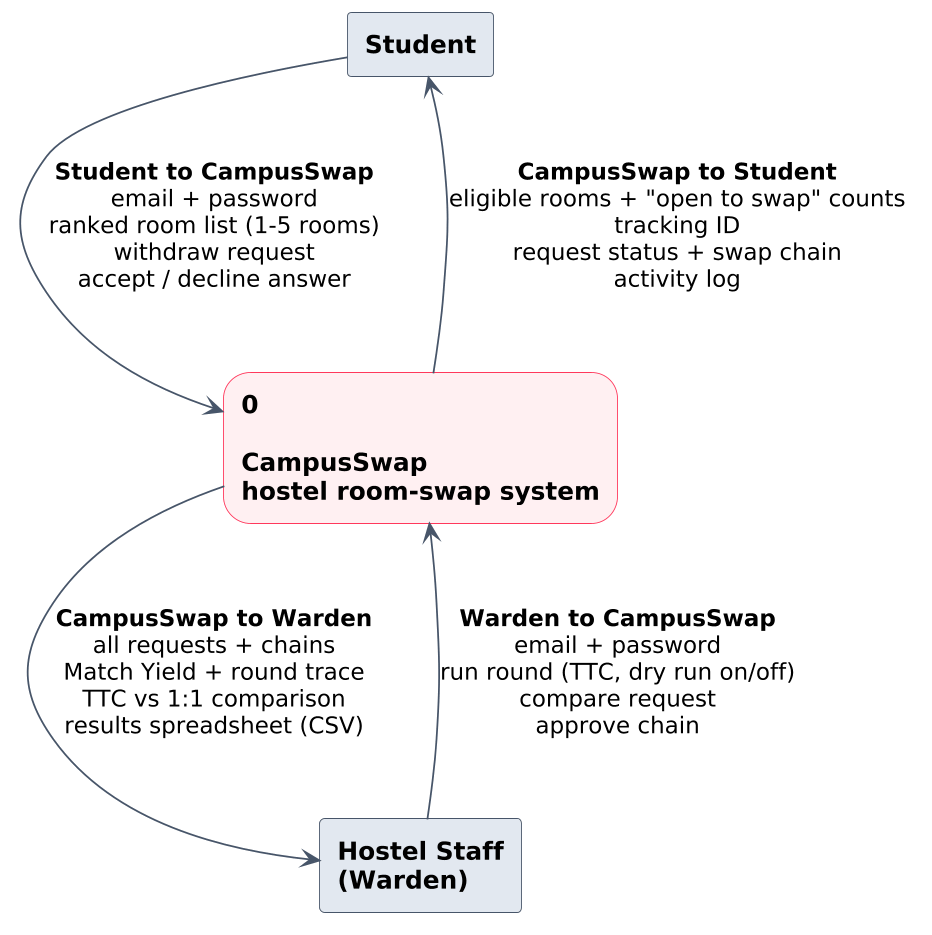
\includegraphics[width=0.62\linewidth]{dfd-context}
  \caption[Context diagram (data flow diagram, Level 0)]{Context diagram
    (data flow diagram, Level 0). The rounded box is the whole system; the
    square boxes are the people outside it. Each arrow lists the data that
    moves in that direction.}
  \label{fig:context}
\end{figure}

\section{References}

\begin{enumerate}[label={[\arabic*]},ref={\arabic*},leftmargin=2.2em]
  \item IEEE, \emph{IEEE Recommended Practice for Software Requirements
    Specifications}, IEEE Std 830-1998.
  \item K.~Wiegers and J.~Beatty, \emph{Software Requirements}, 3rd ed.,
    Microsoft Press, 2013.
  \item\label{ref:shapley} L.~Shapley and H.~Scarf, ``On cores and indivisibility,''
    \emph{Journal of Mathematical Economics}, vol.~1, no.~1, pp.~23--37,
    1974.
  \item A.~E.~Roth and A.~Postlewaite, ``Weak versus strong domination in a
    market with indivisible goods,'' \emph{Journal of Mathematical
    Economics}, vol.~4, no.~2, pp.~131--137, 1977.
  \item\label{ref:roth82} A.~E.~Roth, ``Incentive compatibility in a market with indivisible
    goods,'' \emph{Economics Letters}, vol.~9, no.~2, pp.~127--132, 1982.
  \item CampusSwap team, \emph{CampusSwap: Project Proposal}, UCS503P,
    Thapar Institute of Engineering and Technology, 2026.
  \item CampusSwap source code and documentation:
    \url{https://github.com/ranvir7123/UCS503P-202627-CampusSwap}.
  \item FastAPI documentation: \url{https://fastapi.tiangolo.com}.
  \item SQLAlchemy 2.0 documentation:
    \url{https://docs.sqlalchemy.org/en/20/}.
\end{enumerate}

% ======================================================================
\chapter{Overall Description}\label{ch:overall}
% ======================================================================

\section{Product Perspective}

CampusSwap is a new, self-contained product. It replaces two informal
processes: swap offers posted in WhatsApp groups, and paper request forms
at the hostel office. It does not replace the hostel office's own
allotment records (see business rule \Req{BR-10}).

The system has three layers and a separate matching engine
(Figure~\ref{fig:architecture}):

\begin{itemize}
  \item \textbf{Pages} in the web browser show data and send the user's
    actions to the server. They contain no business rules.
  \item \textbf{The server} checks who is signed in, applies every rule,
    and stores data in a database.
  \item \textbf{The matching engine} runs Top Trading Cycles. It knows
    nothing about the database or the web, so it can be tested on its own
    with made-up data and reused later (for example, for exchanging
    faculty lecture slots).
\end{itemize}

\begin{figure}[tbp]
  \centering
  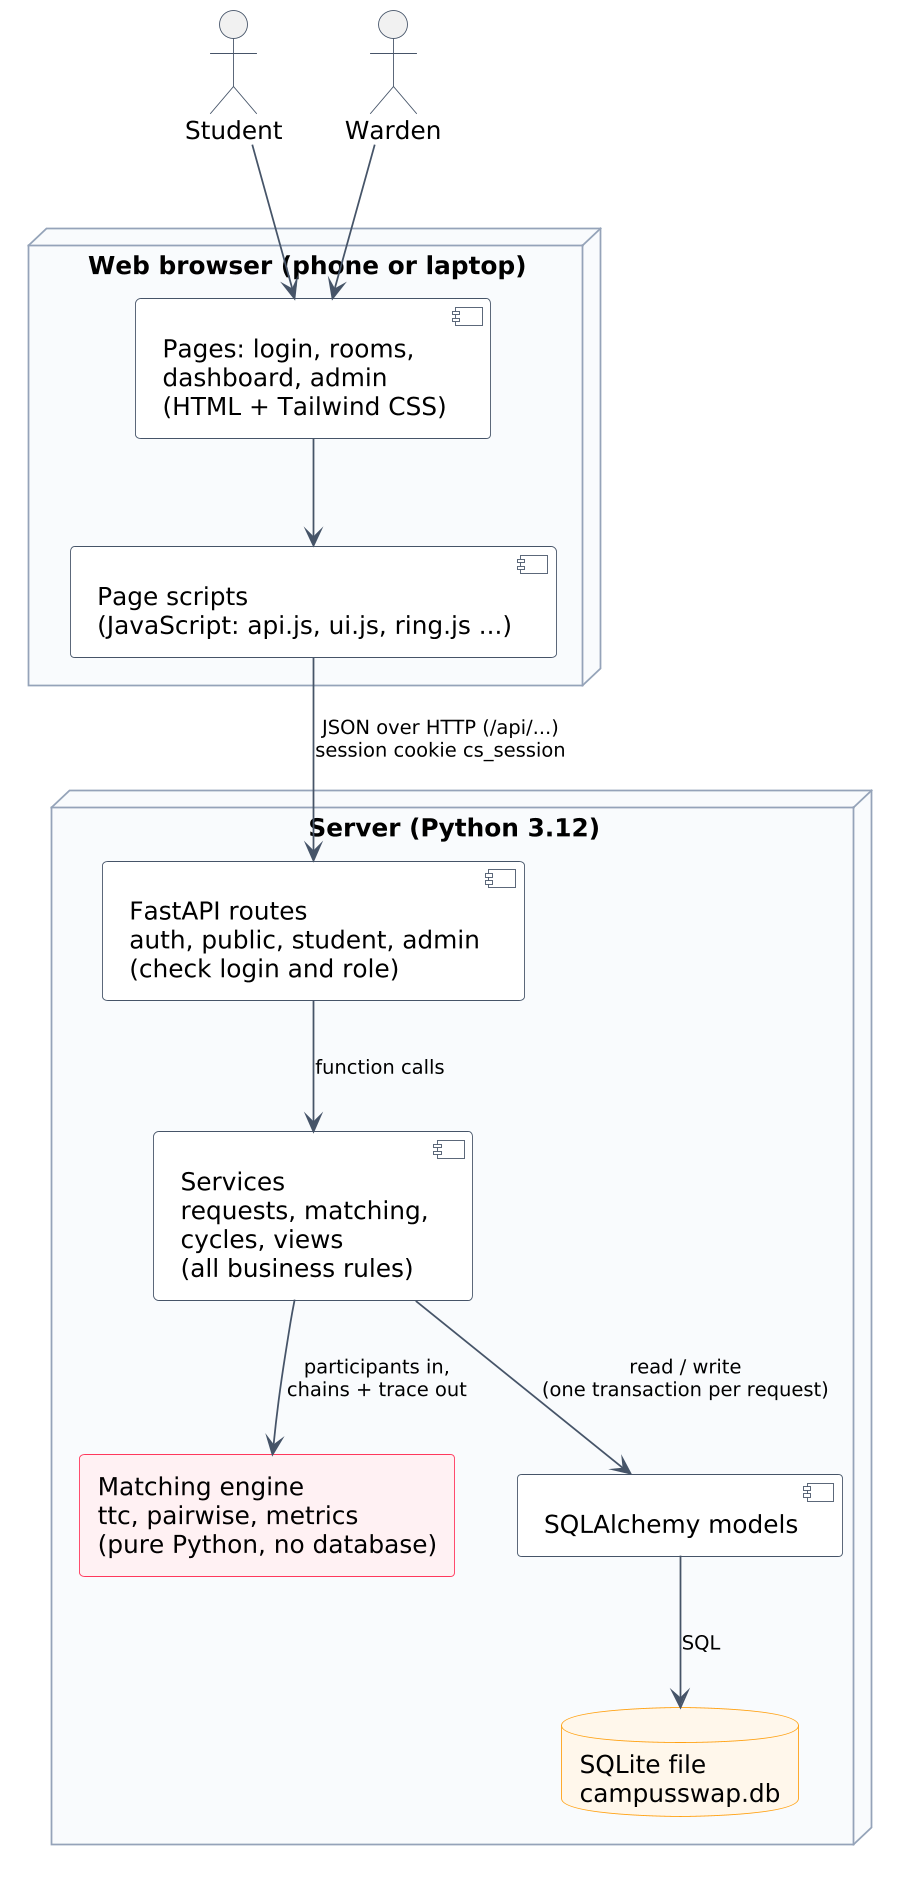
\includegraphics[width=0.46\linewidth]{architecture}
  \caption[System architecture]{System architecture. Each layer talks only
    to the layer next to it. The matching engine is pure Python and has no
    database code.}
  \label{fig:architecture}
\end{figure}

\section{User Classes and Characteristics}\label{sec:classes}

CampusSwap has two kinds of users. Figure~\ref{fig:usecase} shows what
each one can do.

\begin{xltabular}{\linewidth}{@{}L{2.6cm}L{2.2cm}Y@{}}
  \caption{User classes}\label{tab:users}\\
  \toprule
  \textbf{User class} & \textbf{How many} & \textbf{Characteristics and
    needs}\\
  \midrule
  \endfirsthead
  \toprule
  \textbf{User class} & \textbf{How many} & \textbf{Characteristics and
    needs}\\
  \midrule
  \endhead
  Student & Hundreds per hostel; most important class & Already lives in
    a hostel room (owns one bed, called a \emph{seat}). Usually uses a
    phone. Not technical. Wants a better room, wants to know whether
    anything is happening, and wants to keep their current room if no
    good swap exists. Uses the system a few times a semester.\\
  Hostel Staff (Warden) & One office per group of hostels & Runs matching
    rounds, checks the results, approves confirmed swaps and exports
    records. Uses a laptop. Needs a clear record of who asked for what and
    why each swap was proposed.\\
  Visitor (not signed in) & Anyone & Sees only the sign-in page and its
    public numbers (open requests, rooms, last round). Sees no personal
    data.\\
  \bottomrule
\end{xltabular}

\begin{sidewaysfigure}
  \centering
  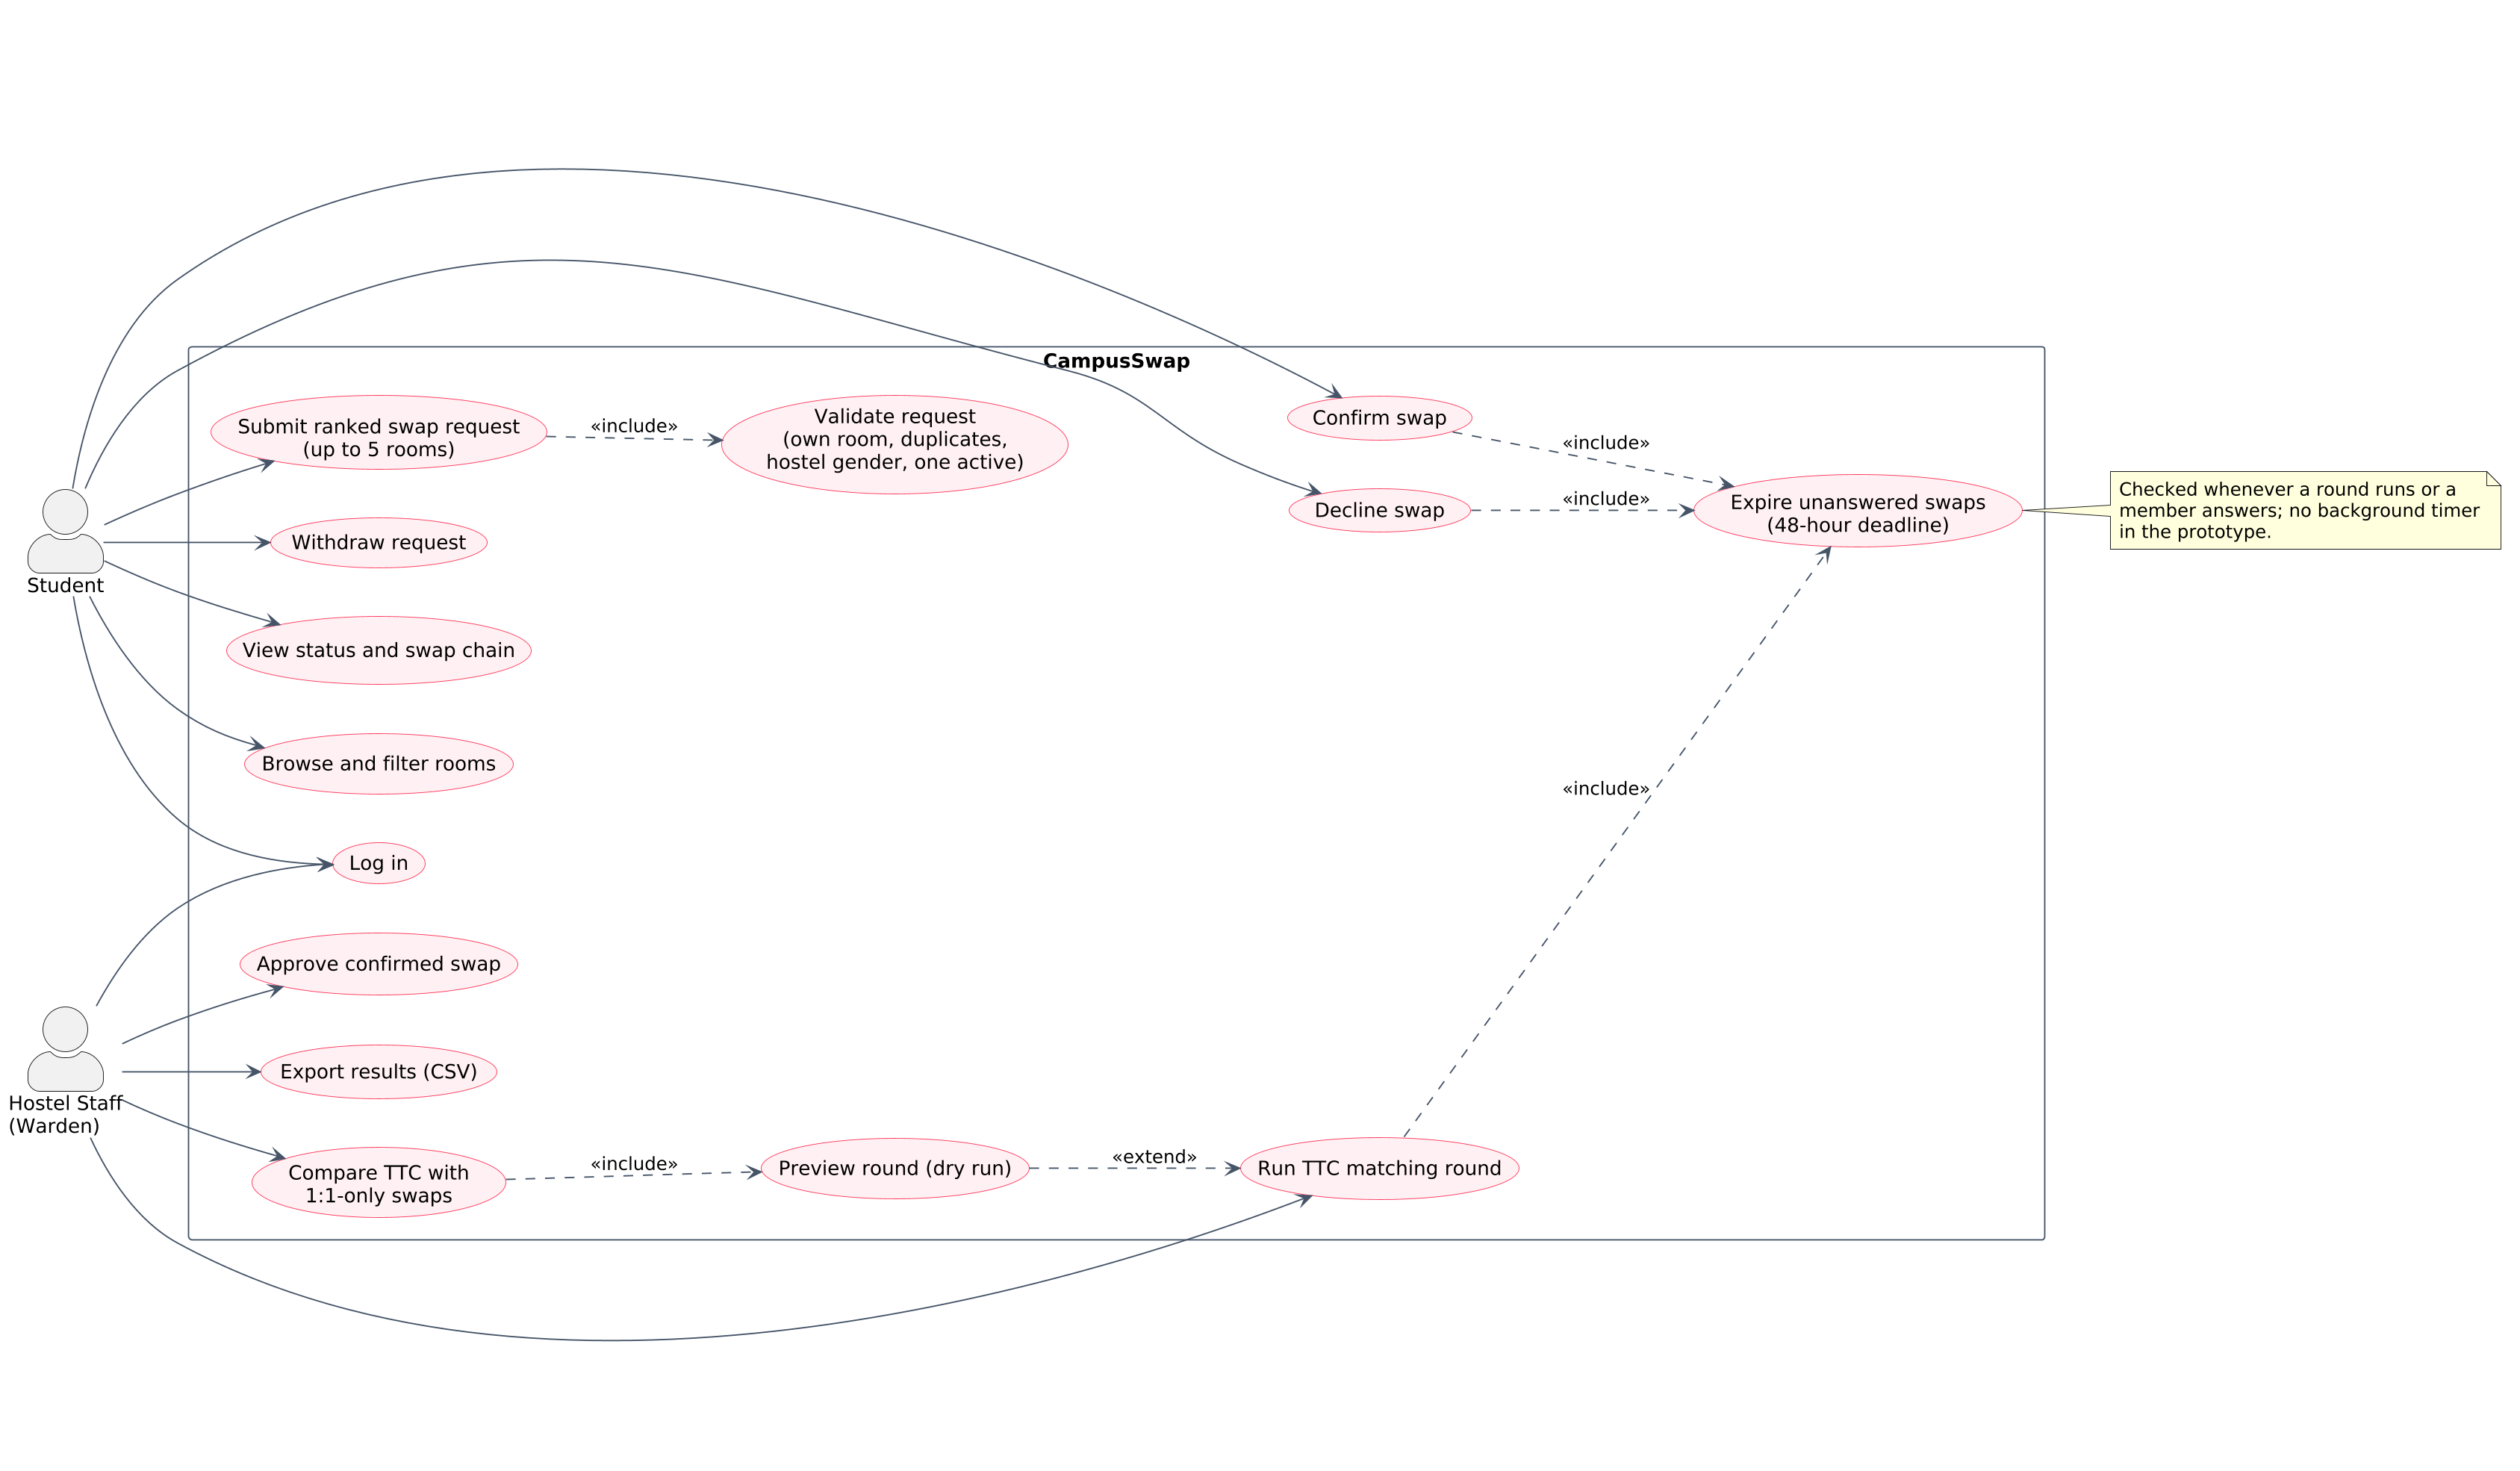
\includegraphics[width=\textheight,height=0.86\textwidth,keepaspectratio]{use-case}
  \caption[Use case diagram]{Use case diagram. \guillemotleft
    include\guillemotright\ marks a step that always happens as part of
    another use case; \guillemotleft extend\guillemotright\ marks an
    optional variation.}
  \label{fig:usecase}
\end{sidewaysfigure}

\section{Product Functions}

The main functions are:

\begin{enumerate}
  \item \textbf{Sign in} as a student or as hostel staff.
  \item \textbf{Browse rooms} in the hostels the student may live in, with
    filters and a count of how many occupants of each room want to swap.
  \item \textbf{Submit or withdraw a swap request}: a ranked list of one to
    five rooms, saved with a tracking ID such as \texttt{CS-2026-0013}.
  \item \textbf{Run a matching round} (TTC) over every open request, see
    the chains it found, the Match Yield and a step-by-step trace, and
    compare the result with direct one-to-one swaps.
  \item \textbf{Accept or decline} a proposed swap chain within 48 hours.
  \item \textbf{Approve} a chain that every member confirmed, which moves
    each student to their new room.
  \item \textbf{Show status and reports}: the student dashboard, the
    warden's overview and request table, and a CSV export.
\end{enumerate}

Figure~\ref{fig:dfd1} breaks the system into these seven processes and
shows the data each one reads and writes. The system keeps five groups of
data (the data stores D1 to D5). Their full structure is in the ER diagram
(Figure~\ref{fig:er}).

\begin{itemize}
  \item \textbf{D1 Users and sessions}: every account (email, name,
    password hash, role; students also have roll number, gender, year and
    branch) and every signed-in browser.
  \item \textbf{D2 Hostels, rooms and seats}: each hostel's code, name and
    the gender it houses; each room's block, floor, number, number of beds
    (1--3), air conditioning, washroom type and tags; each bed (seat) and
    who sleeps in it.
  \item \textbf{D3 Swap requests and preferences}: the tracking ID, the
    student, the seat they offer, the status, and the ranked rooms.
  \item \textbf{D4 Match runs and swap chains}: each round's settings and
    results (pool size, matched, Match Yield, trace), each chain with its
    status and deadline, and each member's answer.
  \item \textbf{D5 Event log}: a time-stamped line for every important
    change, used for the activity list and the audit trail.
\end{itemize}

\begin{sidewaysfigure}
  \centering
  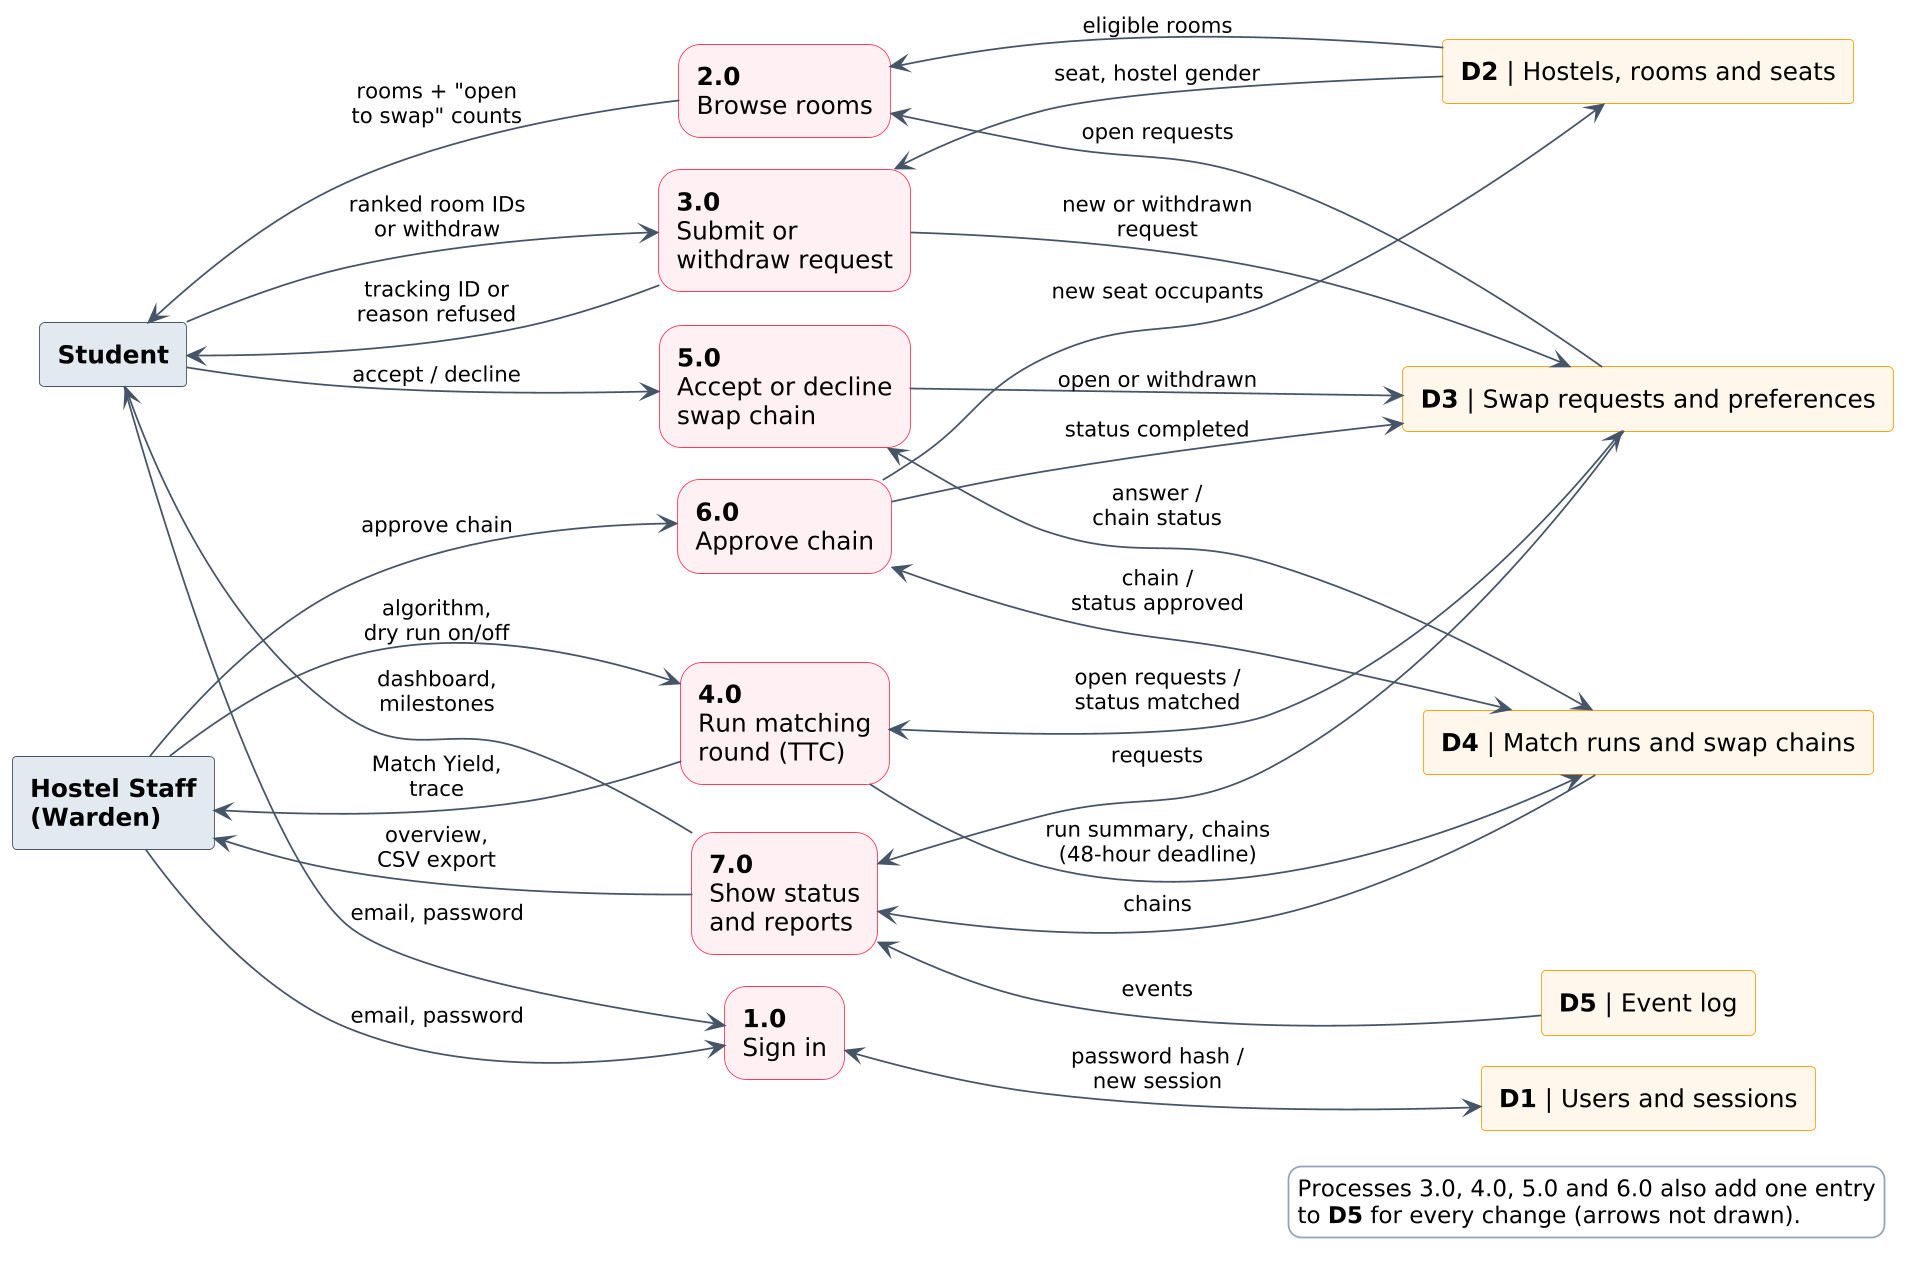
\includegraphics[width=\textheight,height=0.84\textwidth,keepaspectratio]{dfd-level1}
  \caption[Data flow diagram, Level 1]{Data flow diagram, Level 1
    (Gane--Sarson notation). Square boxes are people, rounded boxes are
    processes, and boxes with a D number are data stores. Processes 3.0,
    4.0, 5.0 and 6.0 also add one line to D5 (Event log) for every change;
    those four arrows are left out so the picture stays readable.}
  \label{fig:dfd1}
\end{sidewaysfigure}

\section{Operating Environment}

\begin{itemize}
  \item \textbf{Client:} any current web browser with JavaScript turned on,
    on a phone, tablet or laptop. The pages were checked in Microsoft Edge
    at a desktop width of 1440~pixels and a phone width of 390~pixels.
  \item \textbf{Server:} any computer that runs Python~3.12 or newer
    (Windows, Linux or macOS). By default the server listens on
    \texttt{127.0.0.1}, port \texttt{8000}; both can be changed with
    \texttt{--host} and \texttt{--port}.
  \item \textbf{Database:} one SQLite file, \texttt{campusswap.db}. Nothing
    else needs to be installed.
  \item \textbf{Network:} the pages work without internet access. Fonts,
    icons and style sheets are stored with the application, not loaded
    from other websites.
\end{itemize}

\section{Design and Implementation Constraints}

\begin{xltabular}{\linewidth}{@{}L{3.4cm}Y@{}}
  \caption{Technology used and why}\label{tab:stack}\\
  \toprule
  \textbf{Part} & \textbf{Choice and reason}\\
  \midrule
  \endfirsthead
  \toprule
  \textbf{Part} & \textbf{Choice and reason}\\
  \midrule
  \endhead
  Server & Python 3.12 with FastAPI 0.141.1, run by Uvicorn 0.52.4. Short,
    readable code, and FastAPI generates an interactive API page at
    \texttt{/docs}.\\
  Database & SQLite through SQLAlchemy 2.0.52. A real SQL database in one
    file; moving to PostgreSQL only needs a different database
    address.\\
  Pages & Plain HTML and JavaScript, styled with Tailwind CSS 3.4.19 built
    on the developer's computer, so no internet is needed during a
    demonstration.\\
  Matching & Top Trading Cycles, as promised in the proposal, written in
    plain Python with no database code.\\
  Testing & pytest 9.1.1 and httpx 0.28.1; GitHub Actions runs every test
    on each push and pull request.\\
  Diagrams & PlantUML text files in \texttt{diagrams/}, drawn into images
    by \texttt{diagrams/render.py}.\\
  \bottomrule
\end{xltabular}

Other constraints:
\begin{itemize}
  \item \textbf{No real student data} may be used in a class project. All
    hostels, names, roll numbers and email addresses in the prototype are
    made up.
  \item The institute's single sign-on (Microsoft account) cannot be used
    without the institute's approval, so the prototype uses its own email
    and password sign-in.
  \item One hostel office uses the system at a time. SQLite allows only
    one writer at a time, which is enough for this.
  \item The project must fit in one semester (2026--27 odd semester).
\end{itemize}

\section{Design}\label{sec:design}

This section describes what each kind of user does, step by step, and how
a request and a swap chain change status over time.

\subsection{Student activities}

\begin{enumerate}
  \item Sign in with a Thapar email address and password.
  \item Browse rooms in the hostels they may live in, using filters.
  \item Rank up to five rooms, best first, and submit. The system checks
    the list and either saves it with a tracking ID or explains what is
    wrong.
  \item Wait in the \emph{pool} until the warden runs a round. While the
    request is still open, the student may withdraw it.
  \item If the round places them in a chain, review the whole chain on the
    dashboard and accept or decline before the 48-hour deadline.
  \item After everyone accepts and the warden approves, see the new room
    on the dashboard.
\end{enumerate}

\subsection{Hostel staff (warden) activities}

\begin{enumerate}
  \item Sign in on the \emph{Hostel Staff} tab.
  \item See the overview: requests in the pool, chains waiting for
    answers, chains waiting for approval, and the last round's results.
  \item Optionally compare TTC with direct one-to-one swaps on the current
    pool, or preview a round without saving it (dry run).
  \item Run a TTC matching round, and read the step-by-step trace that
    explains every chain found.
  \item Approve each chain that every member has confirmed.
  \item Export all requests to a spreadsheet (CSV) for the hostel office.
\end{enumerate}

Figure~\ref{fig:activity} shows both sets of activities together, in
swimlanes, for the life of one request.

\begin{figure}[tbp]
  \centering
  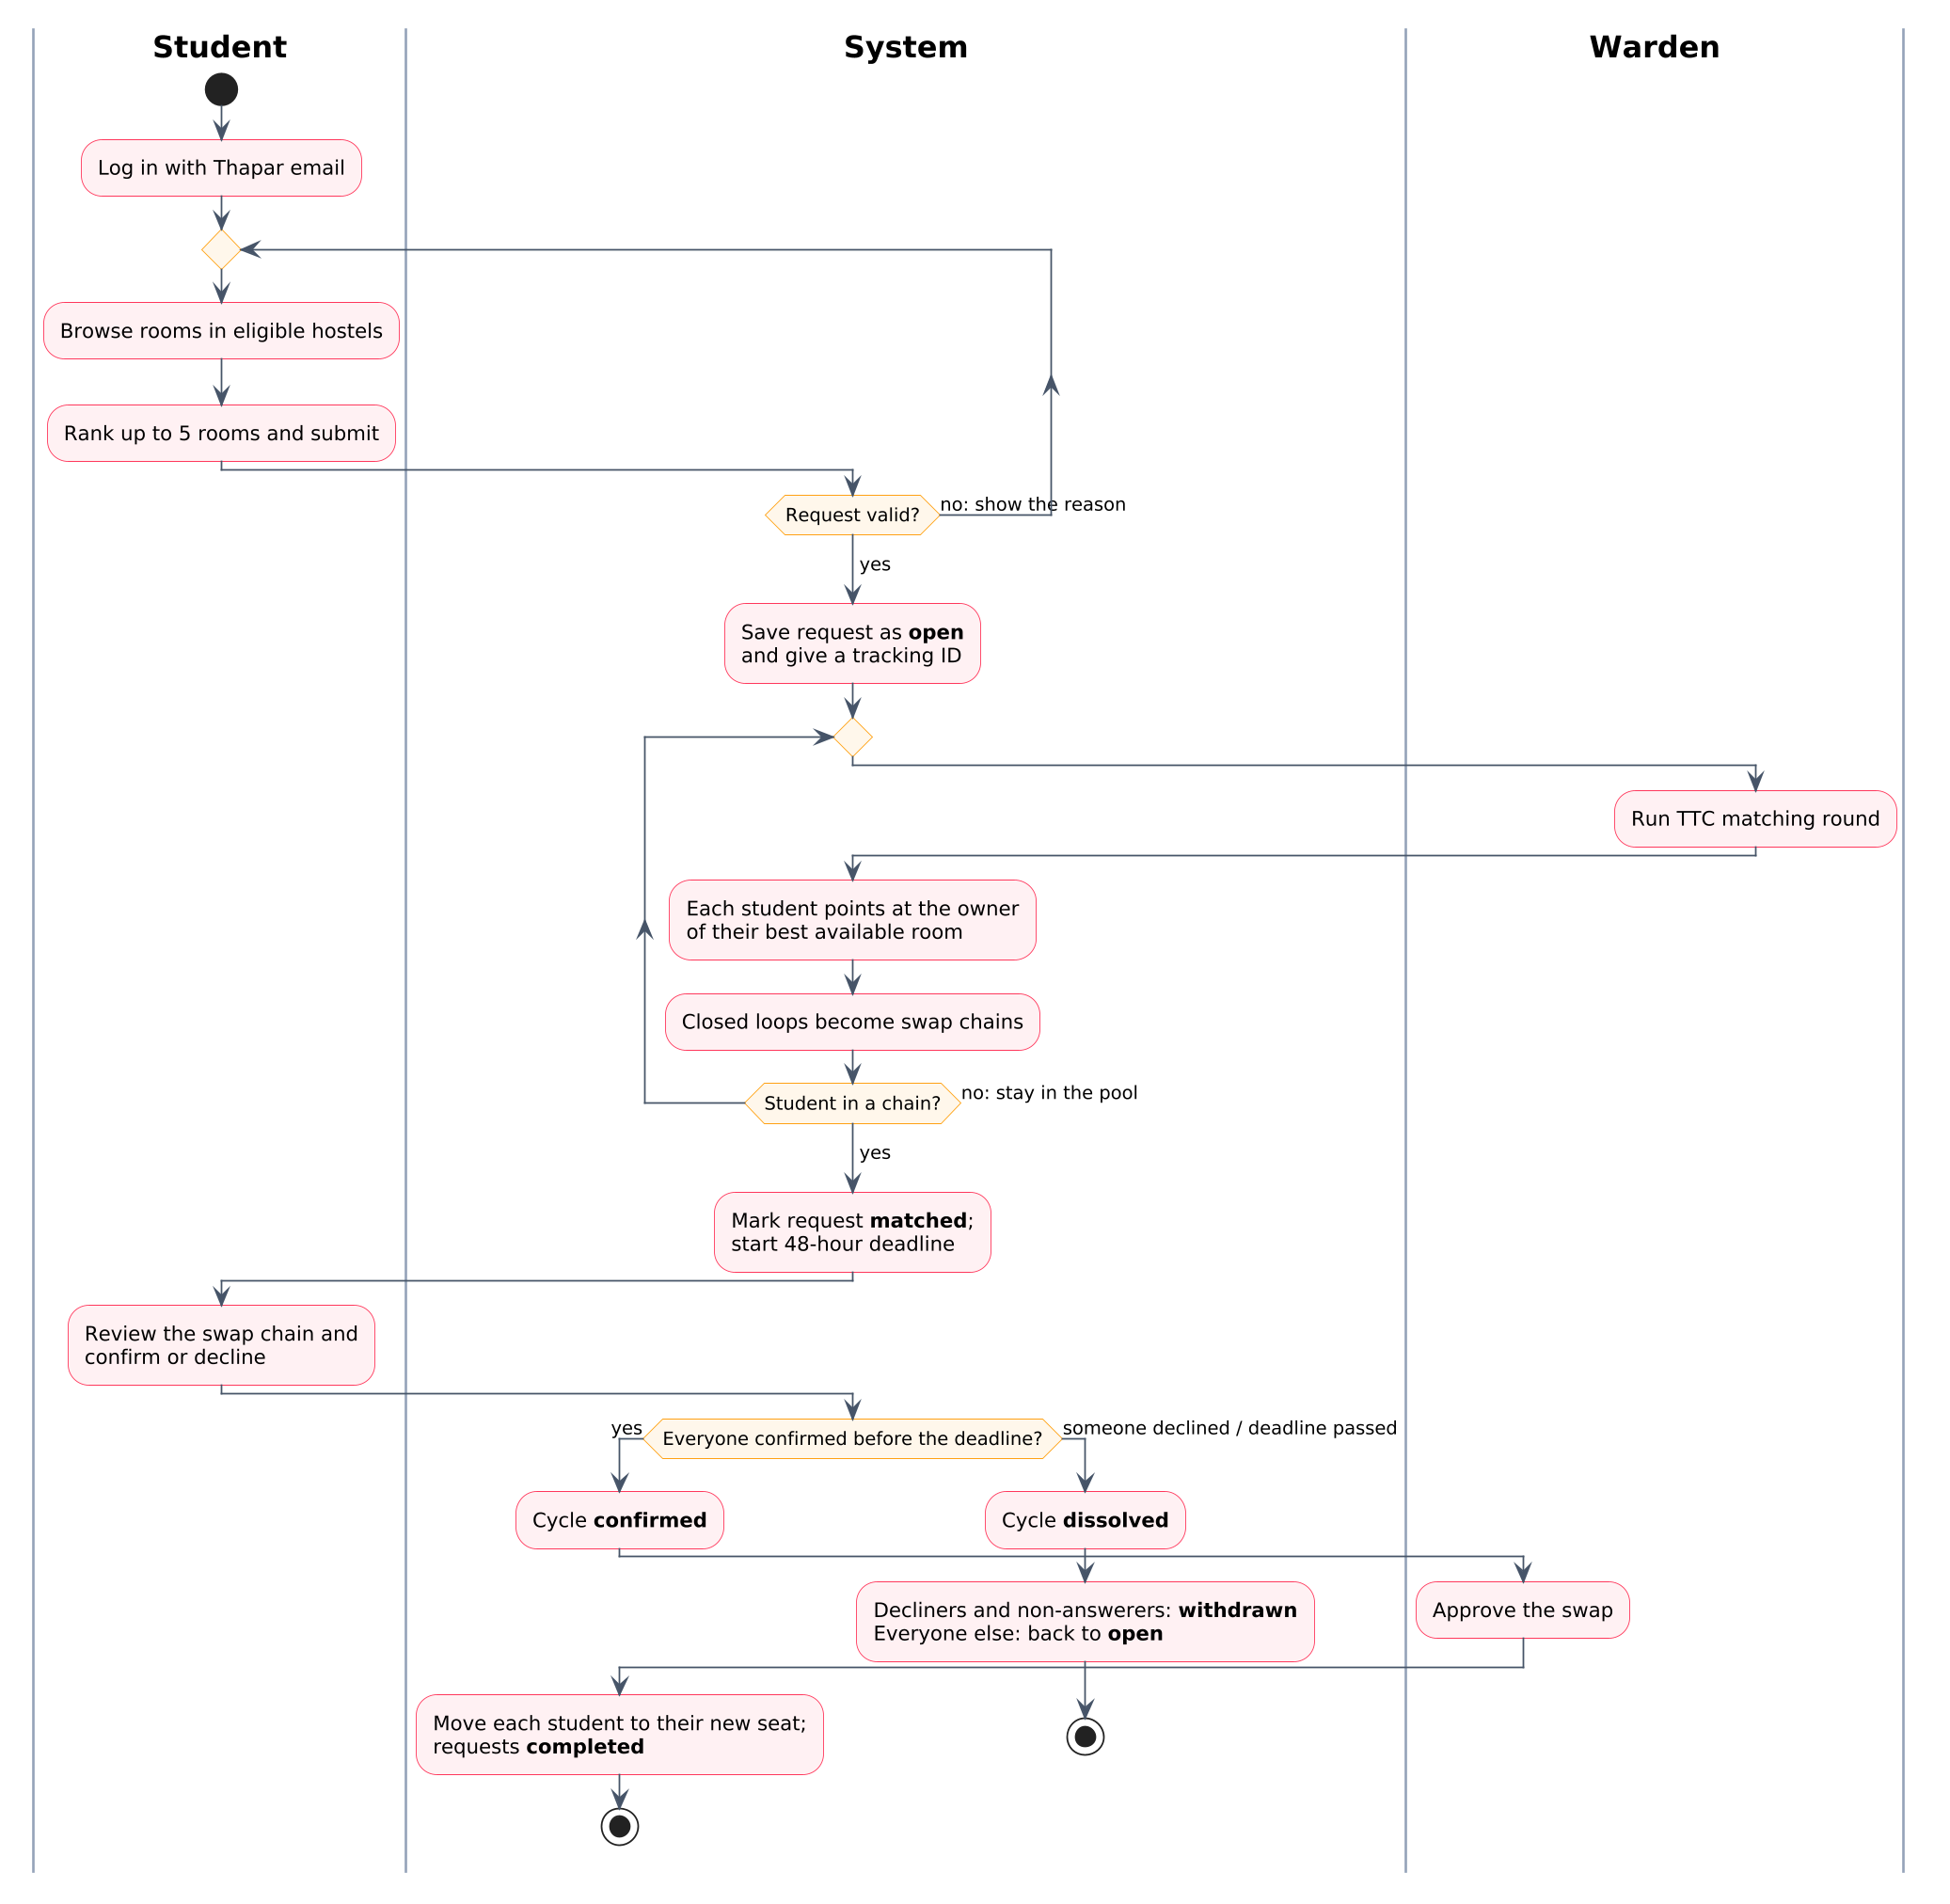
\includegraphics[width=\linewidth]{activity}
  \caption[Activity diagram: life of one swap request]{Activity diagram:
    the life of one swap request, with a swimlane for the student, the
    system and the warden.}
  \label{fig:activity}
\end{figure}

\subsection{How a request and a chain change status}

A swap request is always in one of four states
(Figure~\ref{fig:state-request}). A swap chain, also called a
\emph{cycle}, is always in one of four states
(Figure~\ref{fig:state-cycle}). The two are linked: when a chain is
dissolved, each member's request goes back to \emph{open} or becomes
\emph{withdrawn}, depending on how that member answered.

\begin{figure}[tbp]
  \centering
  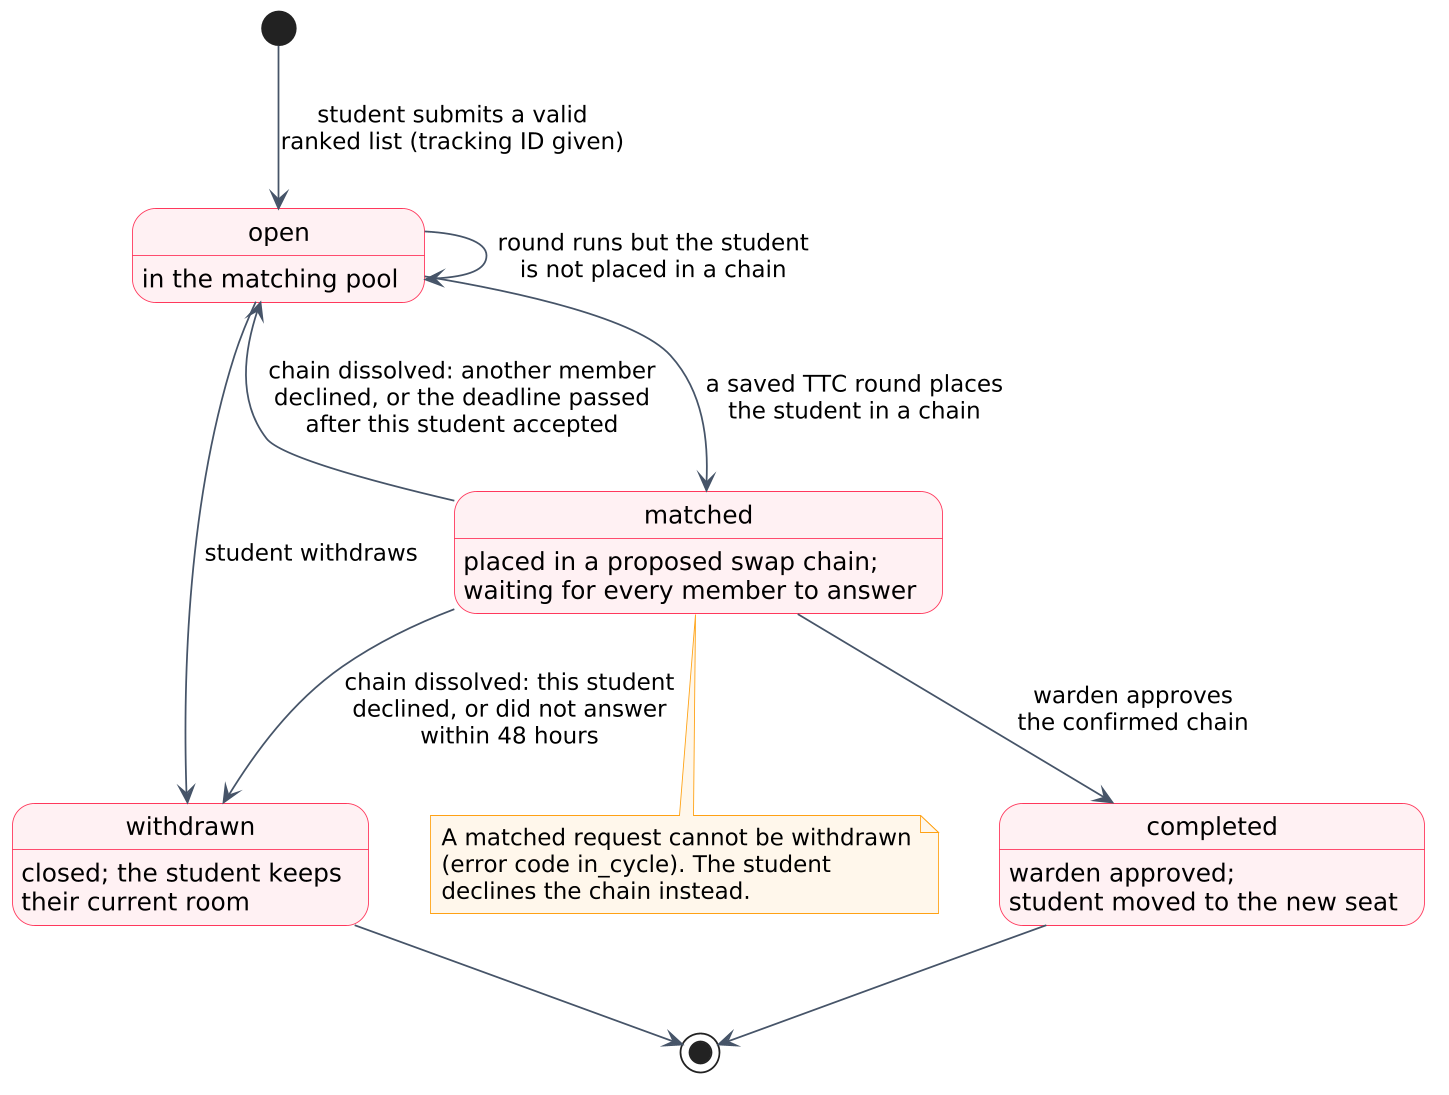
\includegraphics[width=0.80\linewidth]{state-request}
  \caption[State diagram: swap request]{State diagram: the status of one
    swap request.}
  \label{fig:state-request}
\end{figure}

\begin{figure}[tbp]
  \centering
  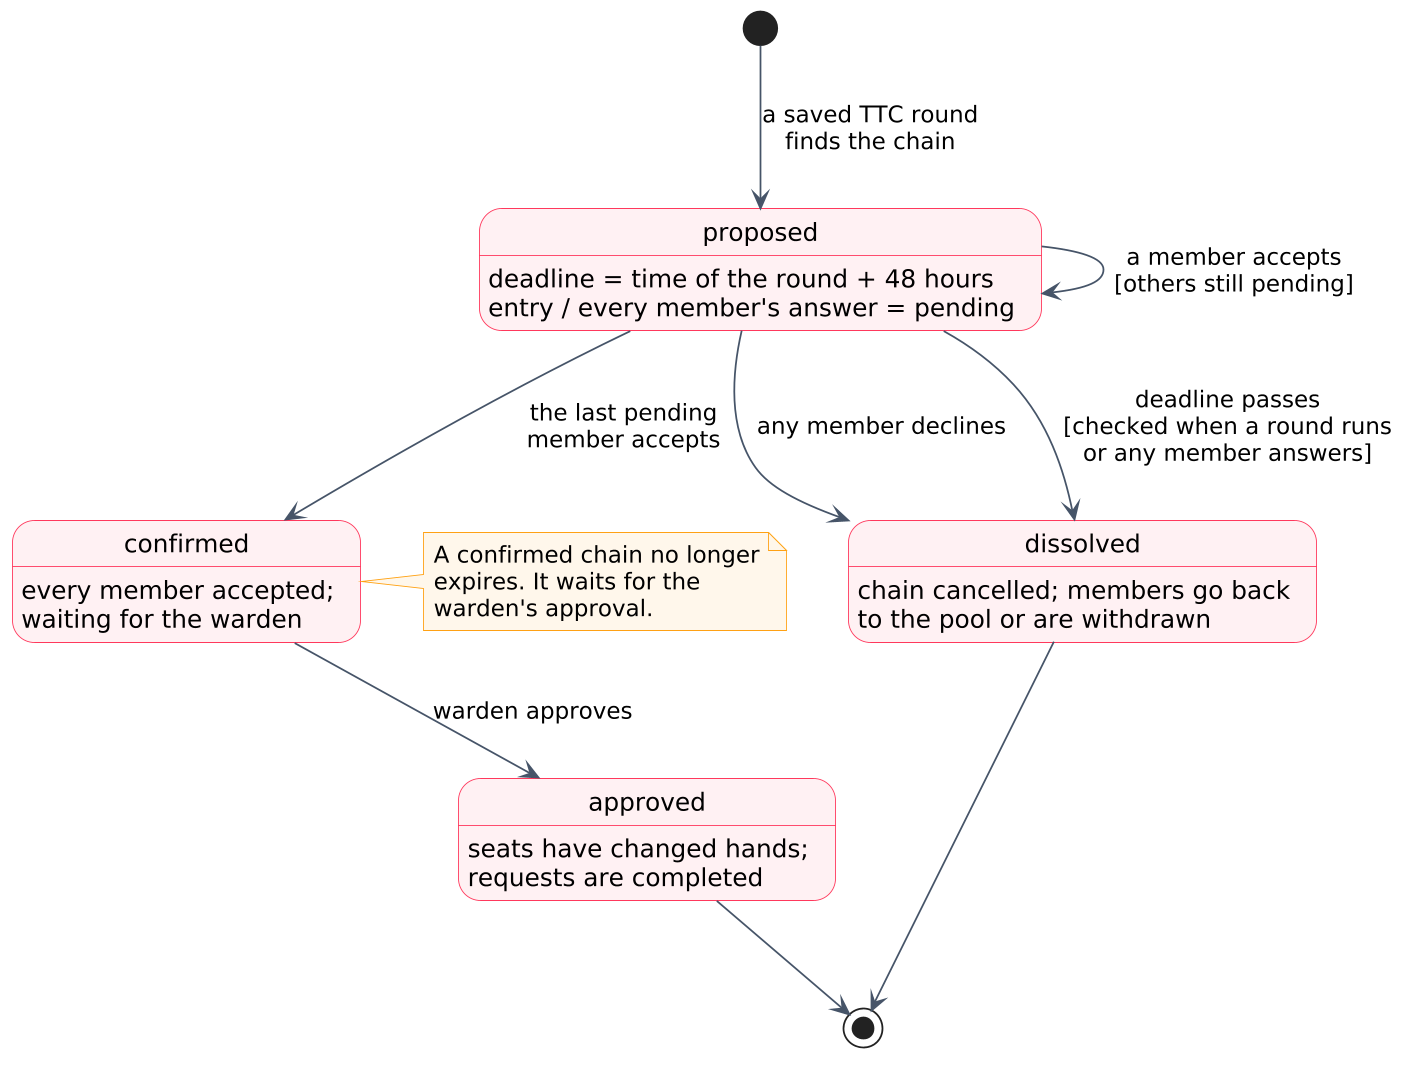
\includegraphics[width=0.78\linewidth]{state-cycle}
  \caption[State diagram: swap chain]{State diagram: the status of one
    swap chain (cycle).}
  \label{fig:state-cycle}
\end{figure}

\subsection{How the parts work together for one swap}

Figure~\ref{fig:sequence} follows one swap from the student's request to
the warden's approval, through the real layers of the system: the page, the
server's routes, the services, the matching engine and the database.

\begin{figure}[tbp]
  \centering
  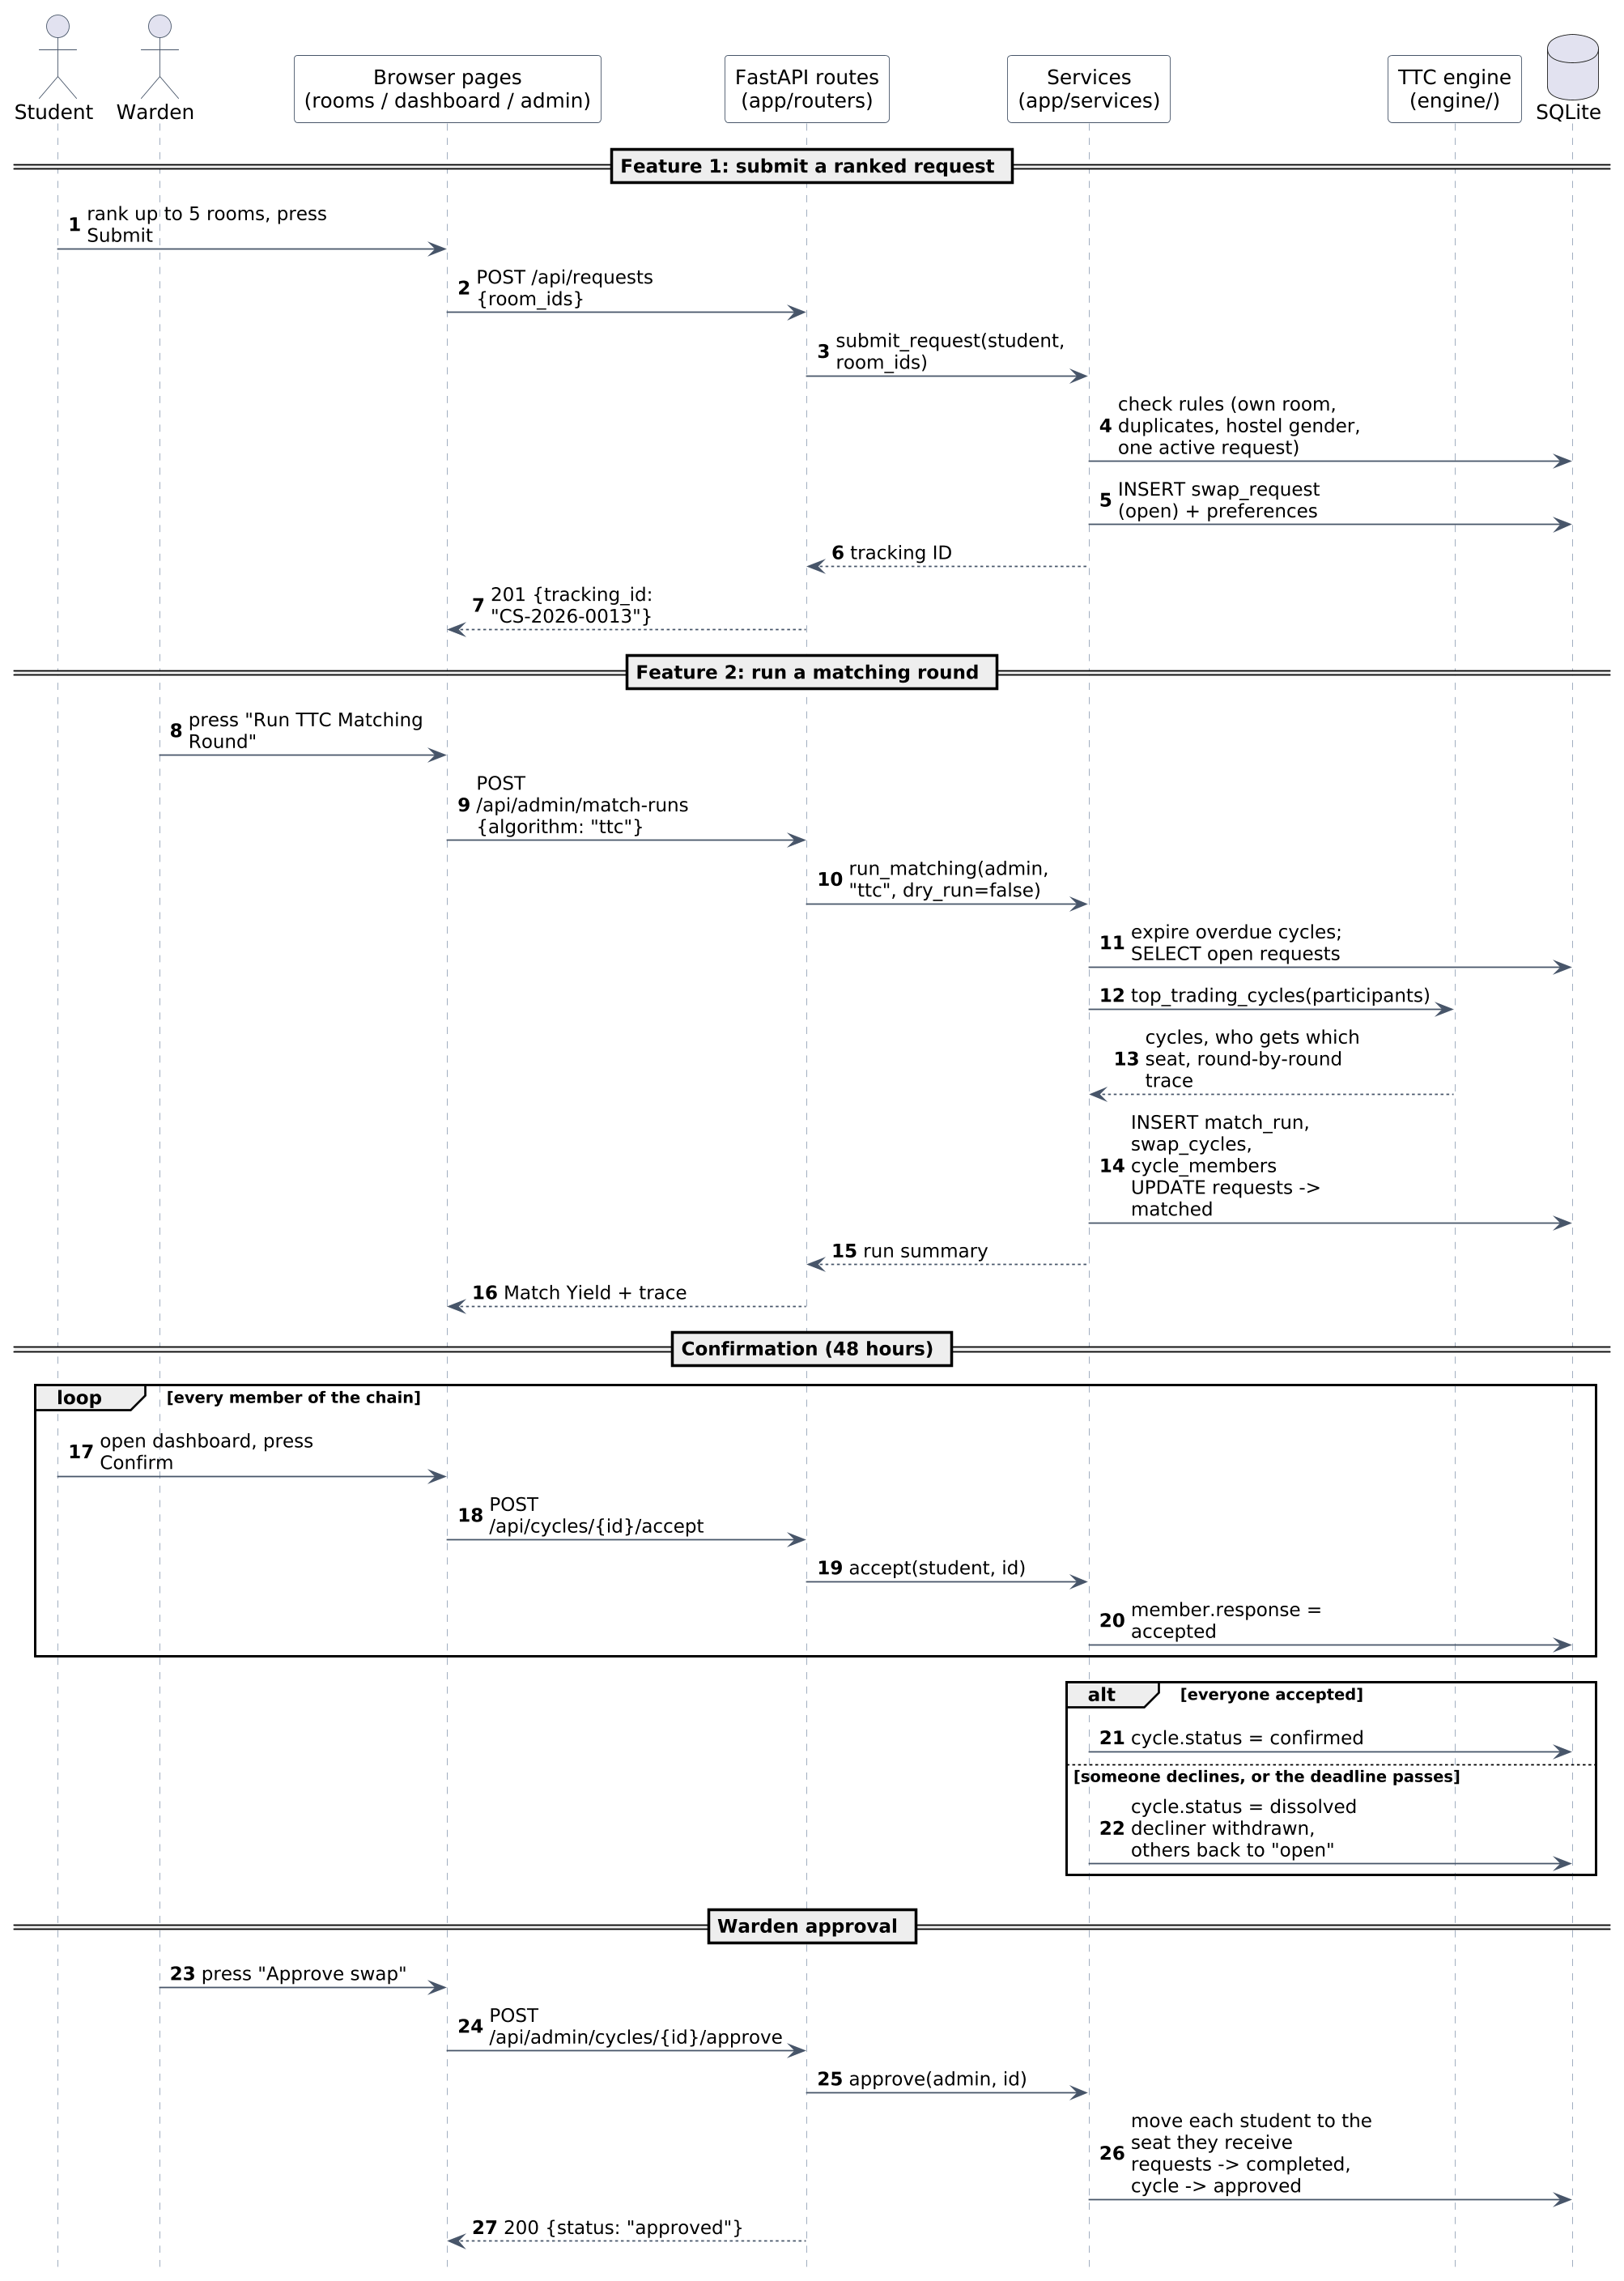
\includegraphics[width=\linewidth]{sequence}
  \caption[Sequence diagram: one swap from request to approval]{Sequence
    diagram: one swap from request to approval. The \emph{loop} box repeats
    for every member of the chain; the \emph{alt} box shows the two ways the
    confirmation step can end.}
  \label{fig:sequence}
\end{figure}

\section{User Documentation}

\begin{itemize}
  \item A documentation website (built with MkDocs from the \texttt{docs/}
    folder) covers getting started, architecture, data model, API,
    matching engine, frontend, testing, diagrams and known limits.
  \item The running server shows an interactive API page at
    \texttt{/docs}, where each call can be tried.
  \item A study guide (\texttt{docs/study/}) explains each part in plain
    language for the four team members.
  \item The sign-in page lists the demo accounts, so a demonstration
    cannot stall on a forgotten password.
\end{itemize}

\section{Assumptions and Dependencies}

\begin{itemize}
  \item Every student who submits a request already occupies exactly one
    seat, and the hostel and room data are correct.
  \item Each hostel houses one gender, and a student may only move within
    hostels of their own gender.
  \item The warden runs matching rounds regularly (for example, weekly).
  \item Until notifications are built (\Req{FR-CONF-06}), students check
    their dashboard within 48 hours of a round.
  \item The hostel office keeps its own master records and copies approved
    swaps into them.
  \item Only development needs the internet: Python packages, GitHub (code
    and automated tests) and the PlantUML server (diagrams).
\end{itemize}

% ======================================================================
\chapter{External Interface Requirements}
% ======================================================================

\section{User Interfaces}\label{sec:ui}

CampusSwap has four pages. The screenshots below come from the working
prototype, running on its made-up demo data after one real matching round.

Rules that every page follows:
\begin{itemize}
  \item While data loads, the page shows grey placeholder shapes (a
    \emph{loading skeleton}) instead of an empty screen.
  \item Every error appears as a short, plain message: a pop-up with the
    server's explanation, or a box on the page with a \emph{Try again}
    button.
  \item Empty states explain what to do next (for example, ``No request
    yet'' with a link to Explore Rooms).
  \item Long names are shortened with ``\ldots'' and shown in full on hover.
  \item Layouts change for phone screens; nothing needs sideways
    scrolling.
\end{itemize}

\begin{figure}[tbp]
  \centering
  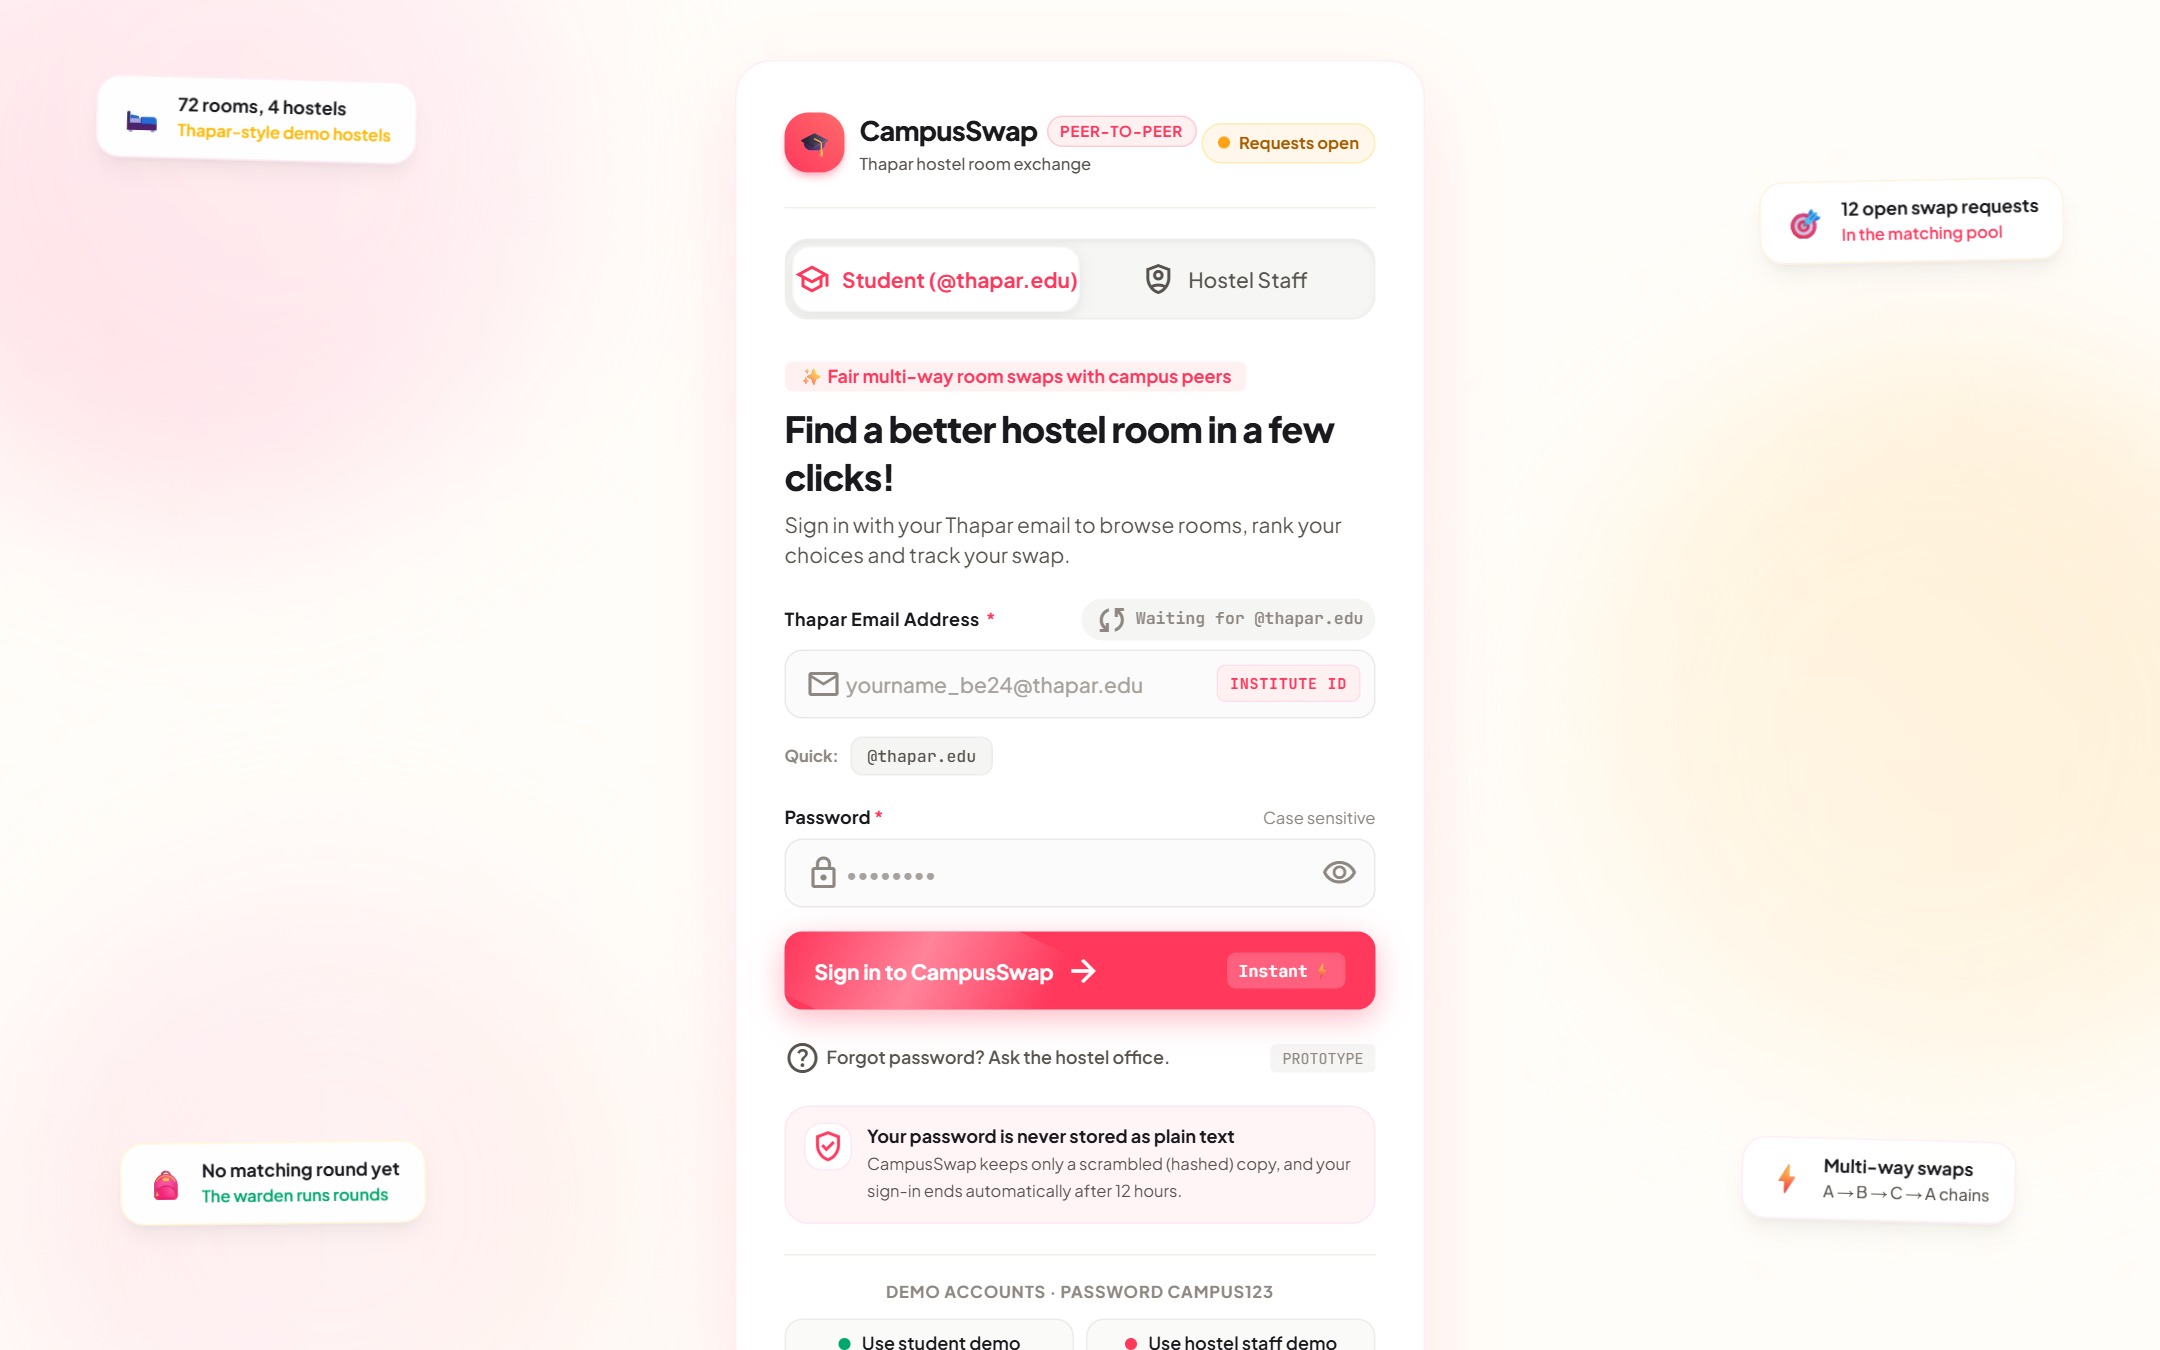
\includegraphics[width=\linewidth]{ui-login}
  \caption[Sign-in page]{Sign-in page. A switch chooses Student or Hostel
    Staff. The floating cards show live public numbers from the server.}
  \label{fig:ui-login}
\end{figure}

\begin{figure}[tbp]
  \centering
  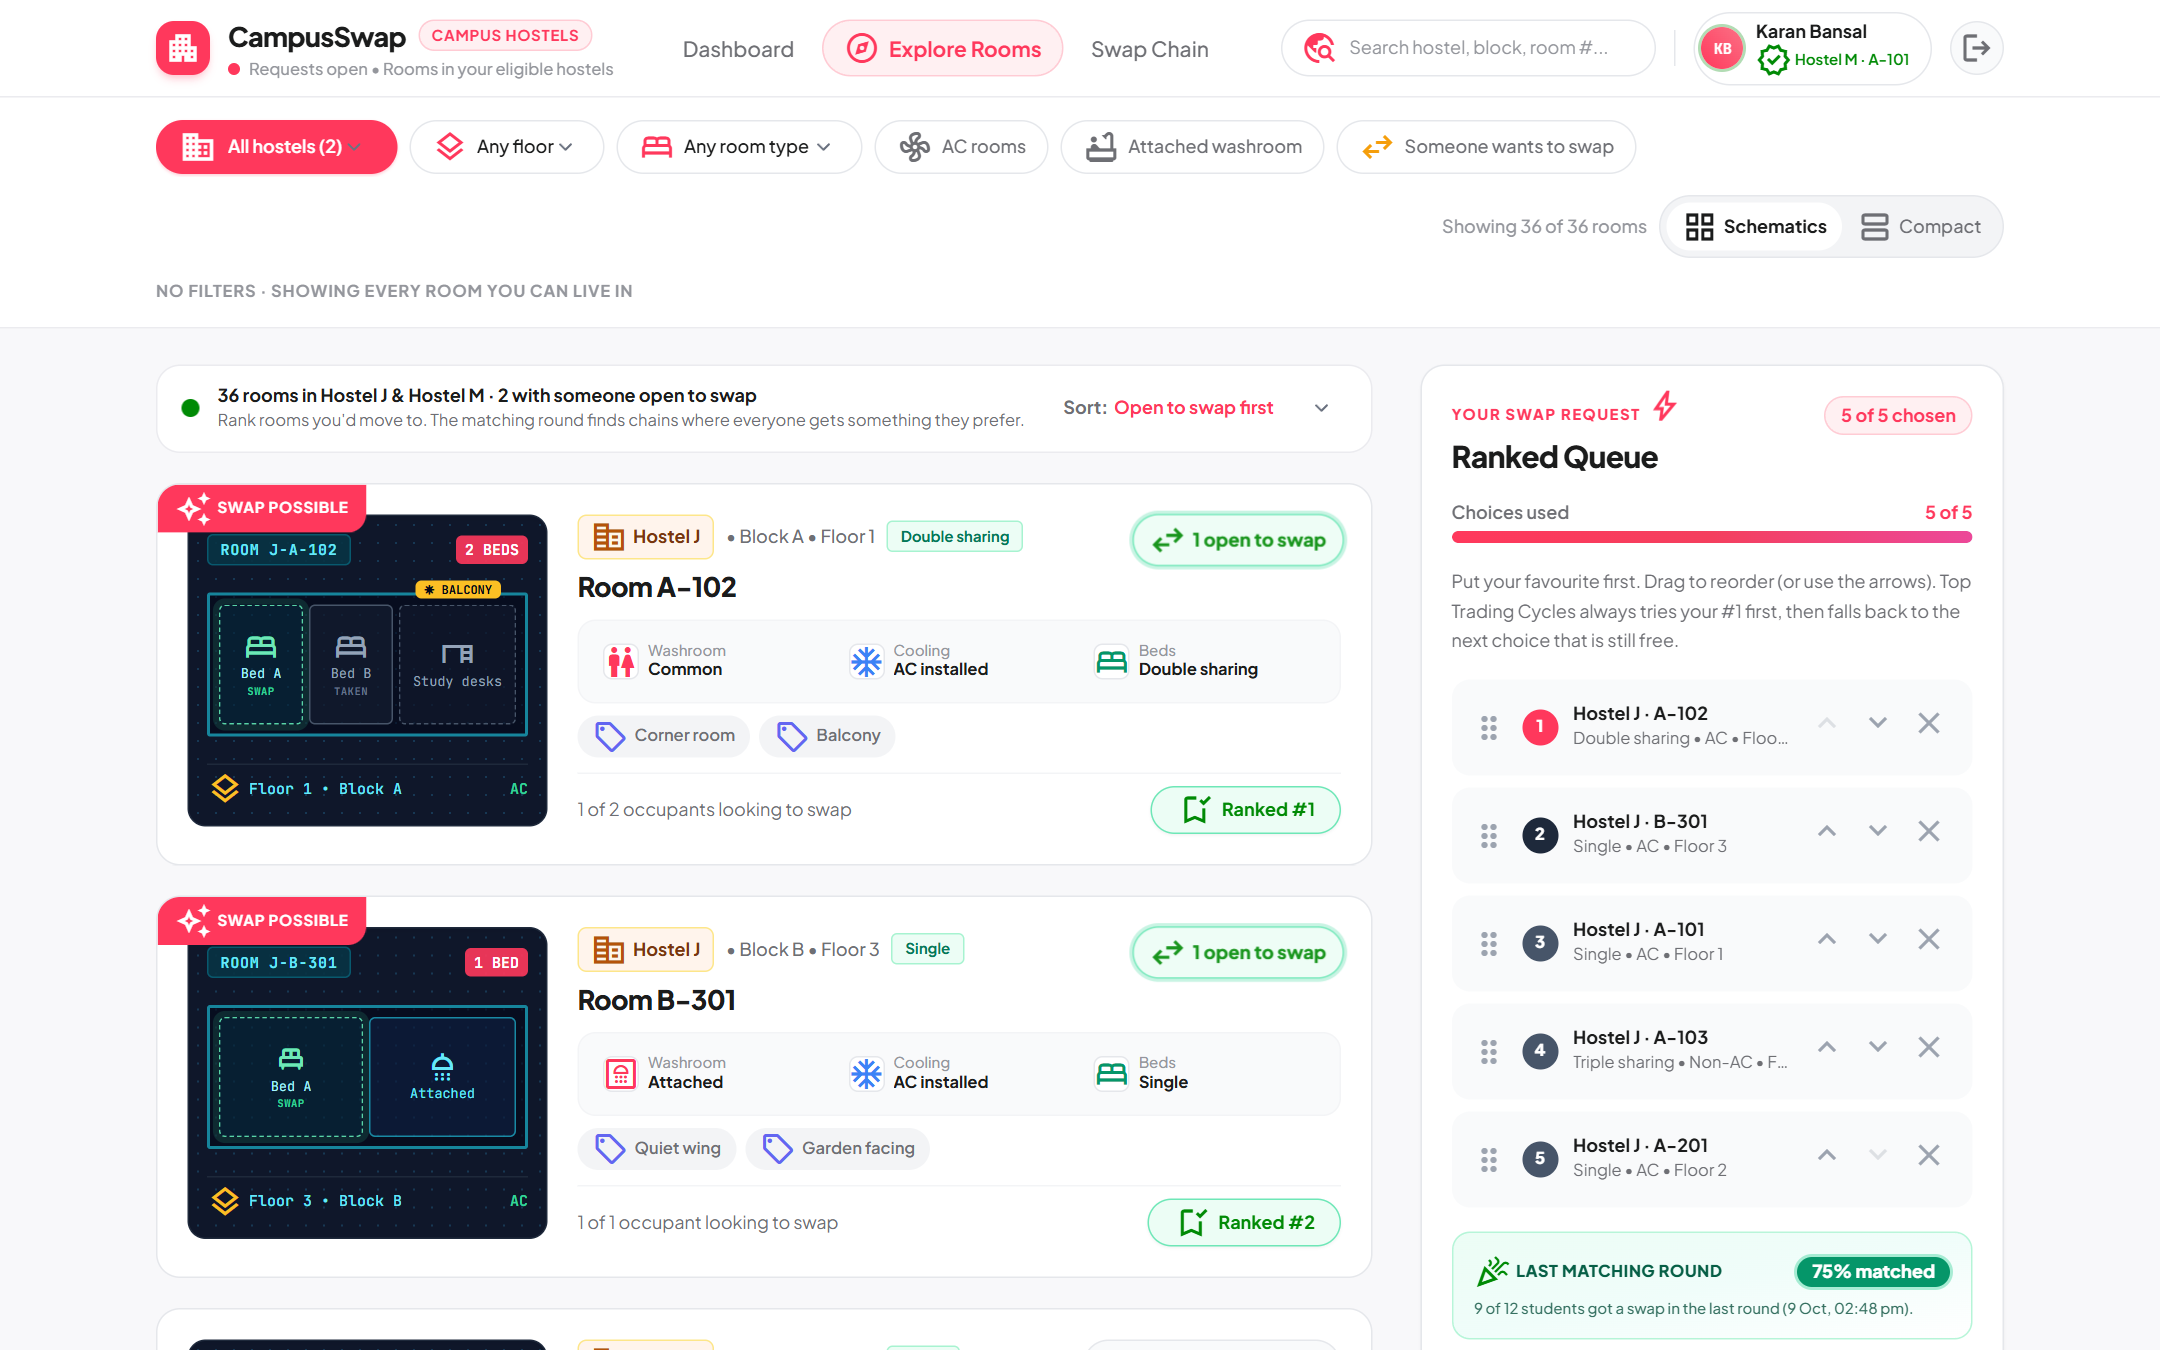
\includegraphics[width=\linewidth]{ui-rooms}
  \caption[Explore Rooms page]{Explore Rooms page. Filters at the top; each
    room card is drawn from the room's data and shows how many occupants
    are open to a swap. The ranked list on the right holds up to five
    choices and can be reordered.}
  \label{fig:ui-rooms}
\end{figure}

\begin{figure}[tbp]
  \centering
  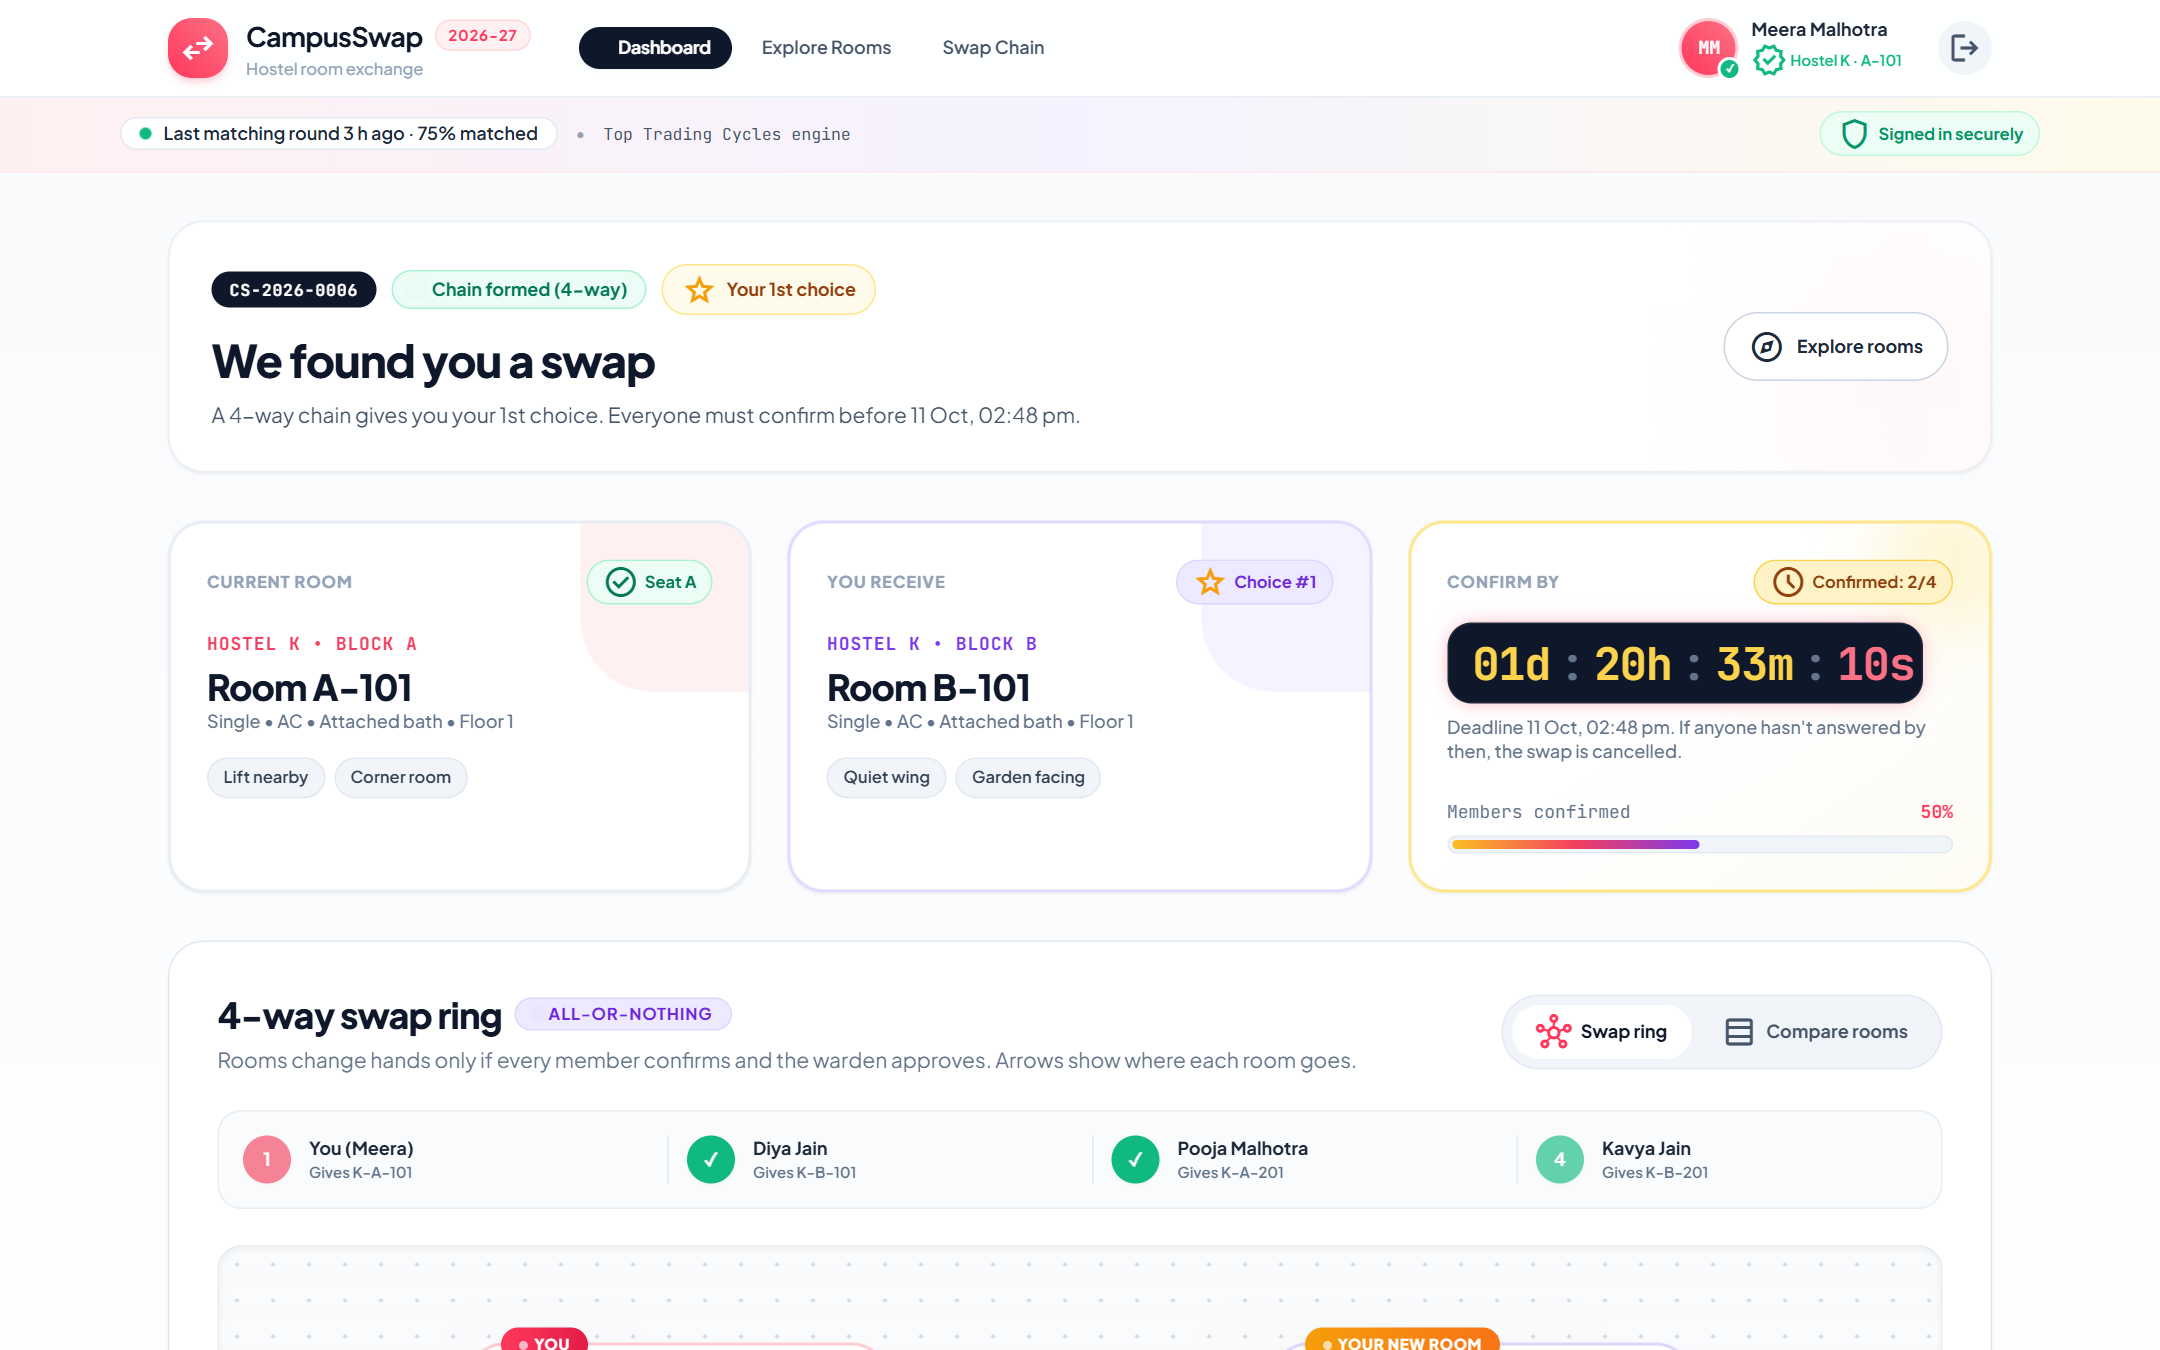
\includegraphics[width=\linewidth]{ui-dashboard}
  \caption[Student dashboard]{Student dashboard after a round: the
    tracking ID, current room, the room on offer, and a countdown to the
    48-hour deadline with how many members have confirmed.}
  \label{fig:ui-dashboard}
\end{figure}

\begin{figure}[tbp]
  \centering
  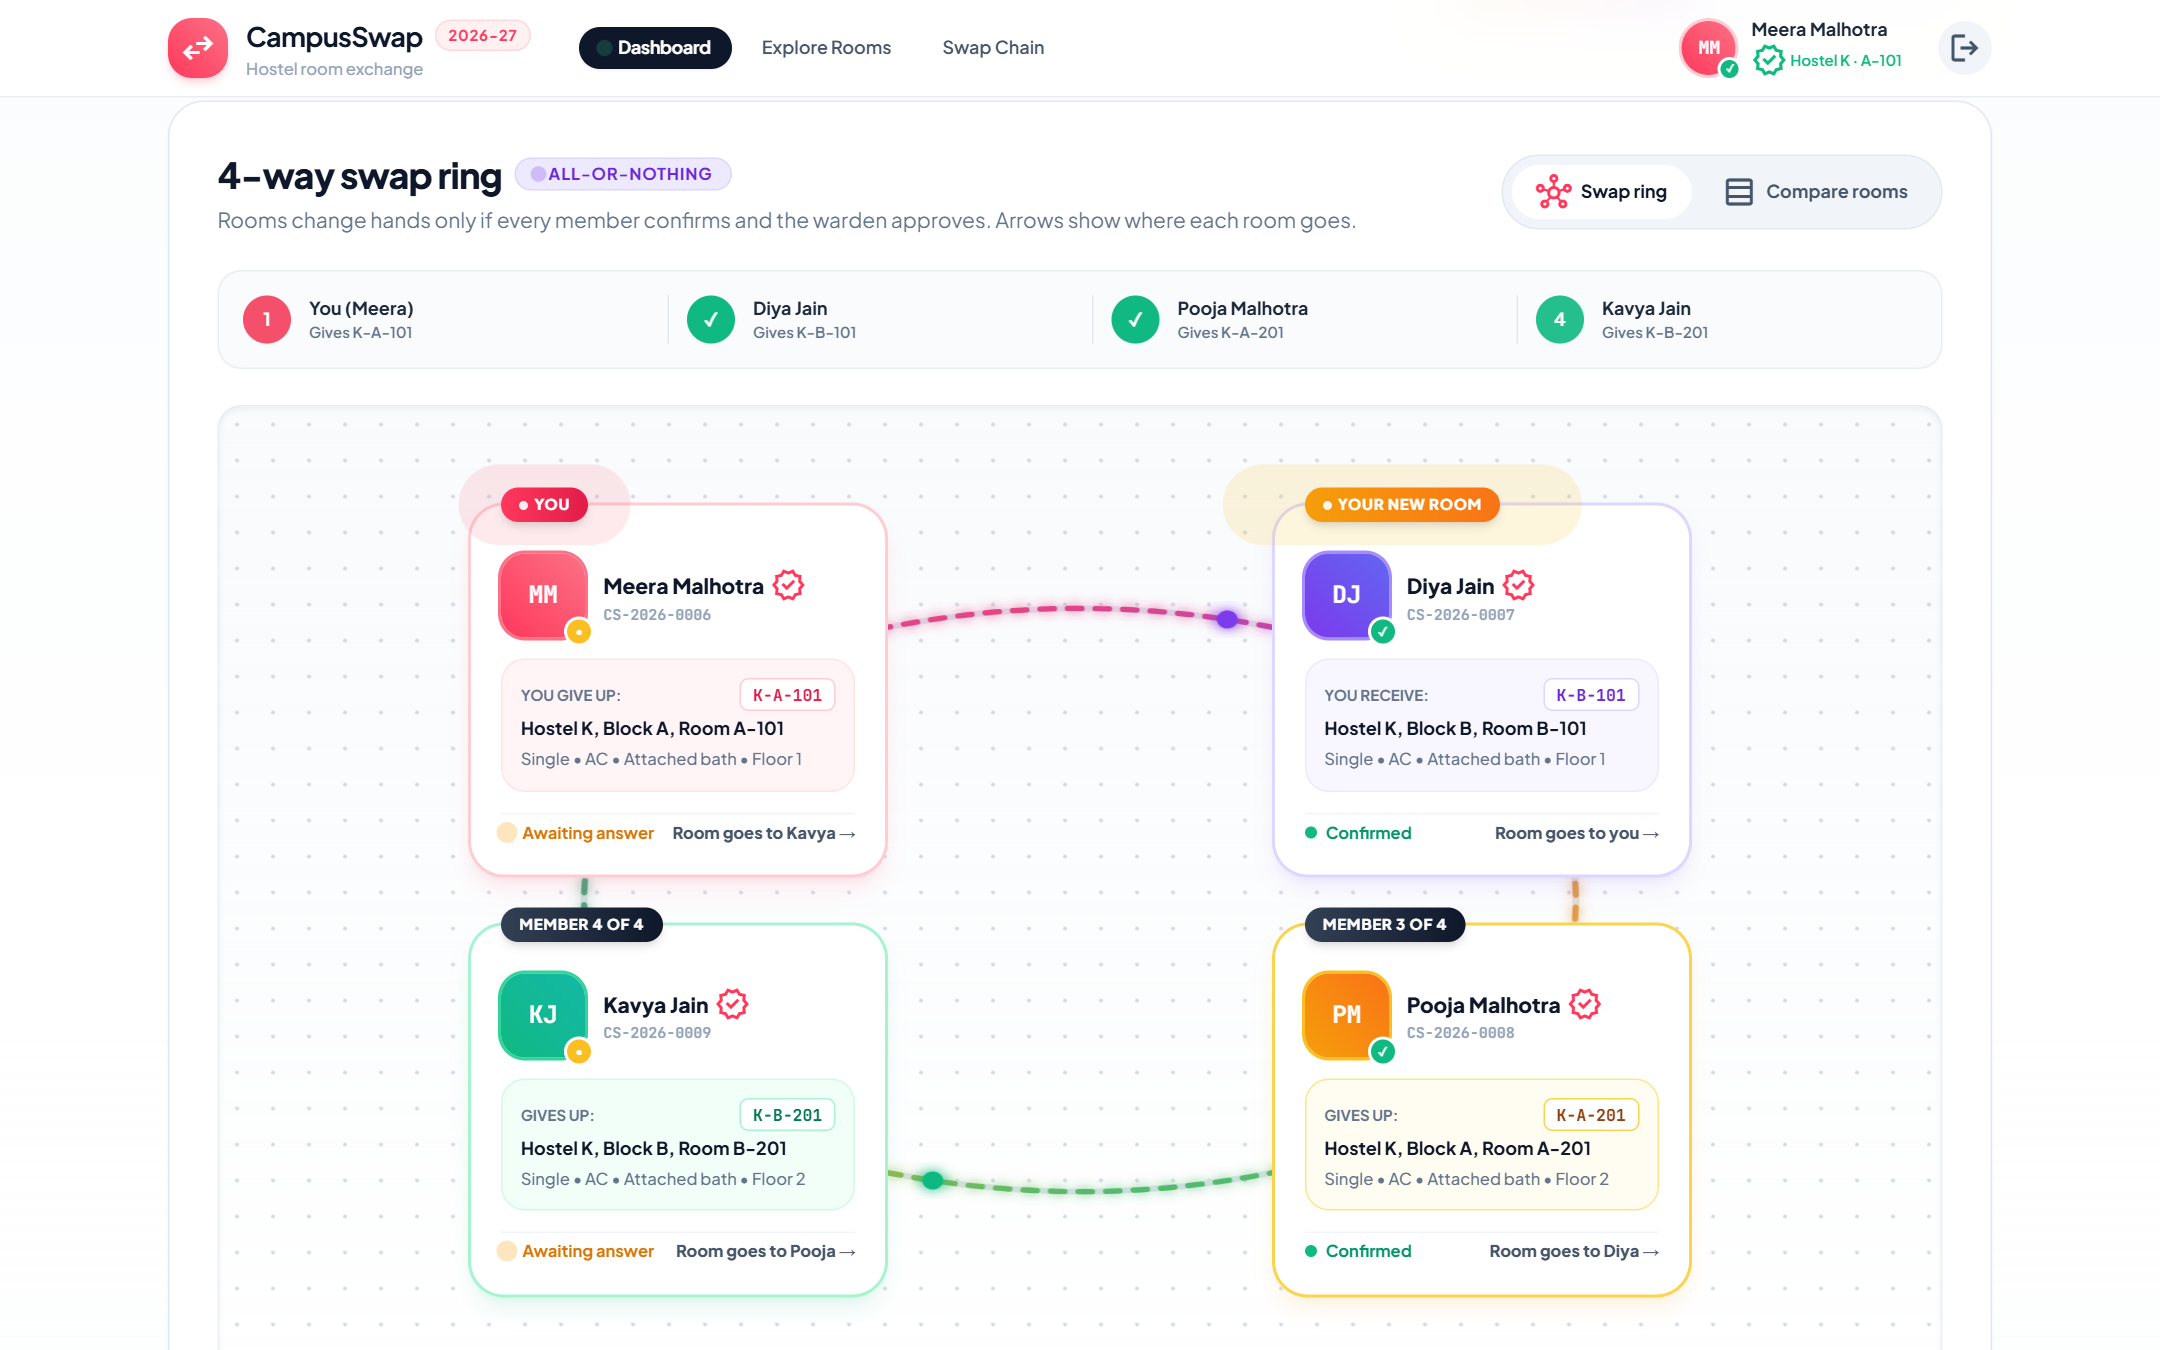
\includegraphics[width=\linewidth]{ui-ring}
  \caption[Swap ring on the student dashboard]{The swap ring for a real
    4-way chain found by the round. Arrows show where each room goes; each
    card shows whether that member has confirmed.}
  \label{fig:ui-ring}
\end{figure}

\begin{figure}[tbp]
  \centering
  \begin{subfigure}[t]{0.32\linewidth}
    \centering
    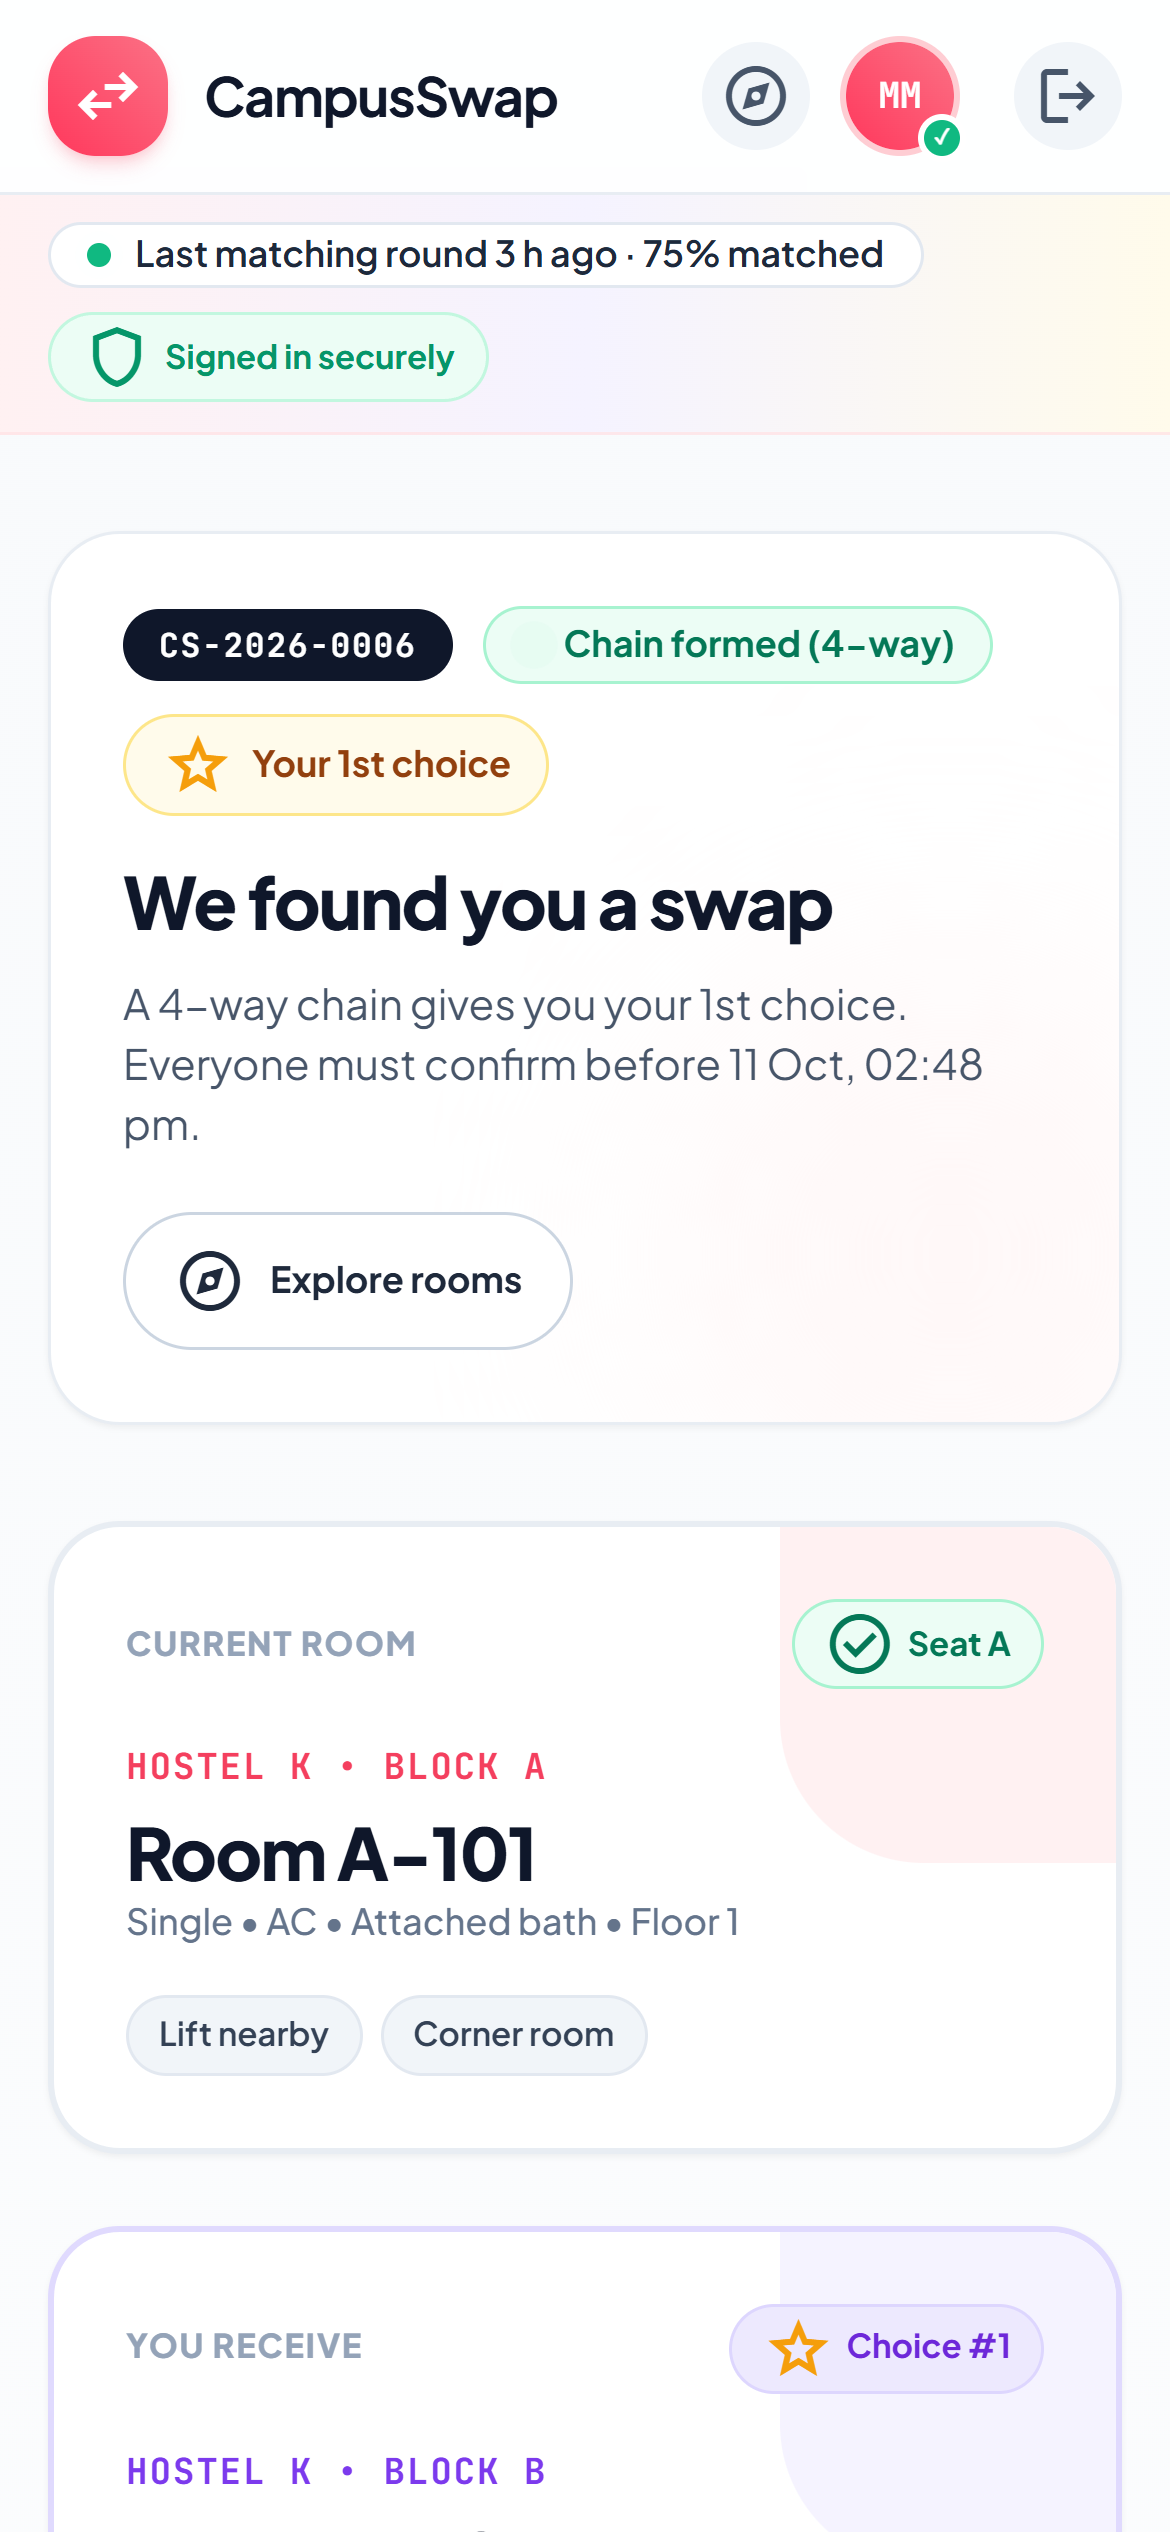
\includegraphics[width=\linewidth]{ui-dashboard-phone}
    \caption{Top of the dashboard}
  \end{subfigure}\hspace{1.2cm}%
  \begin{subfigure}[t]{0.32\linewidth}
    \centering
    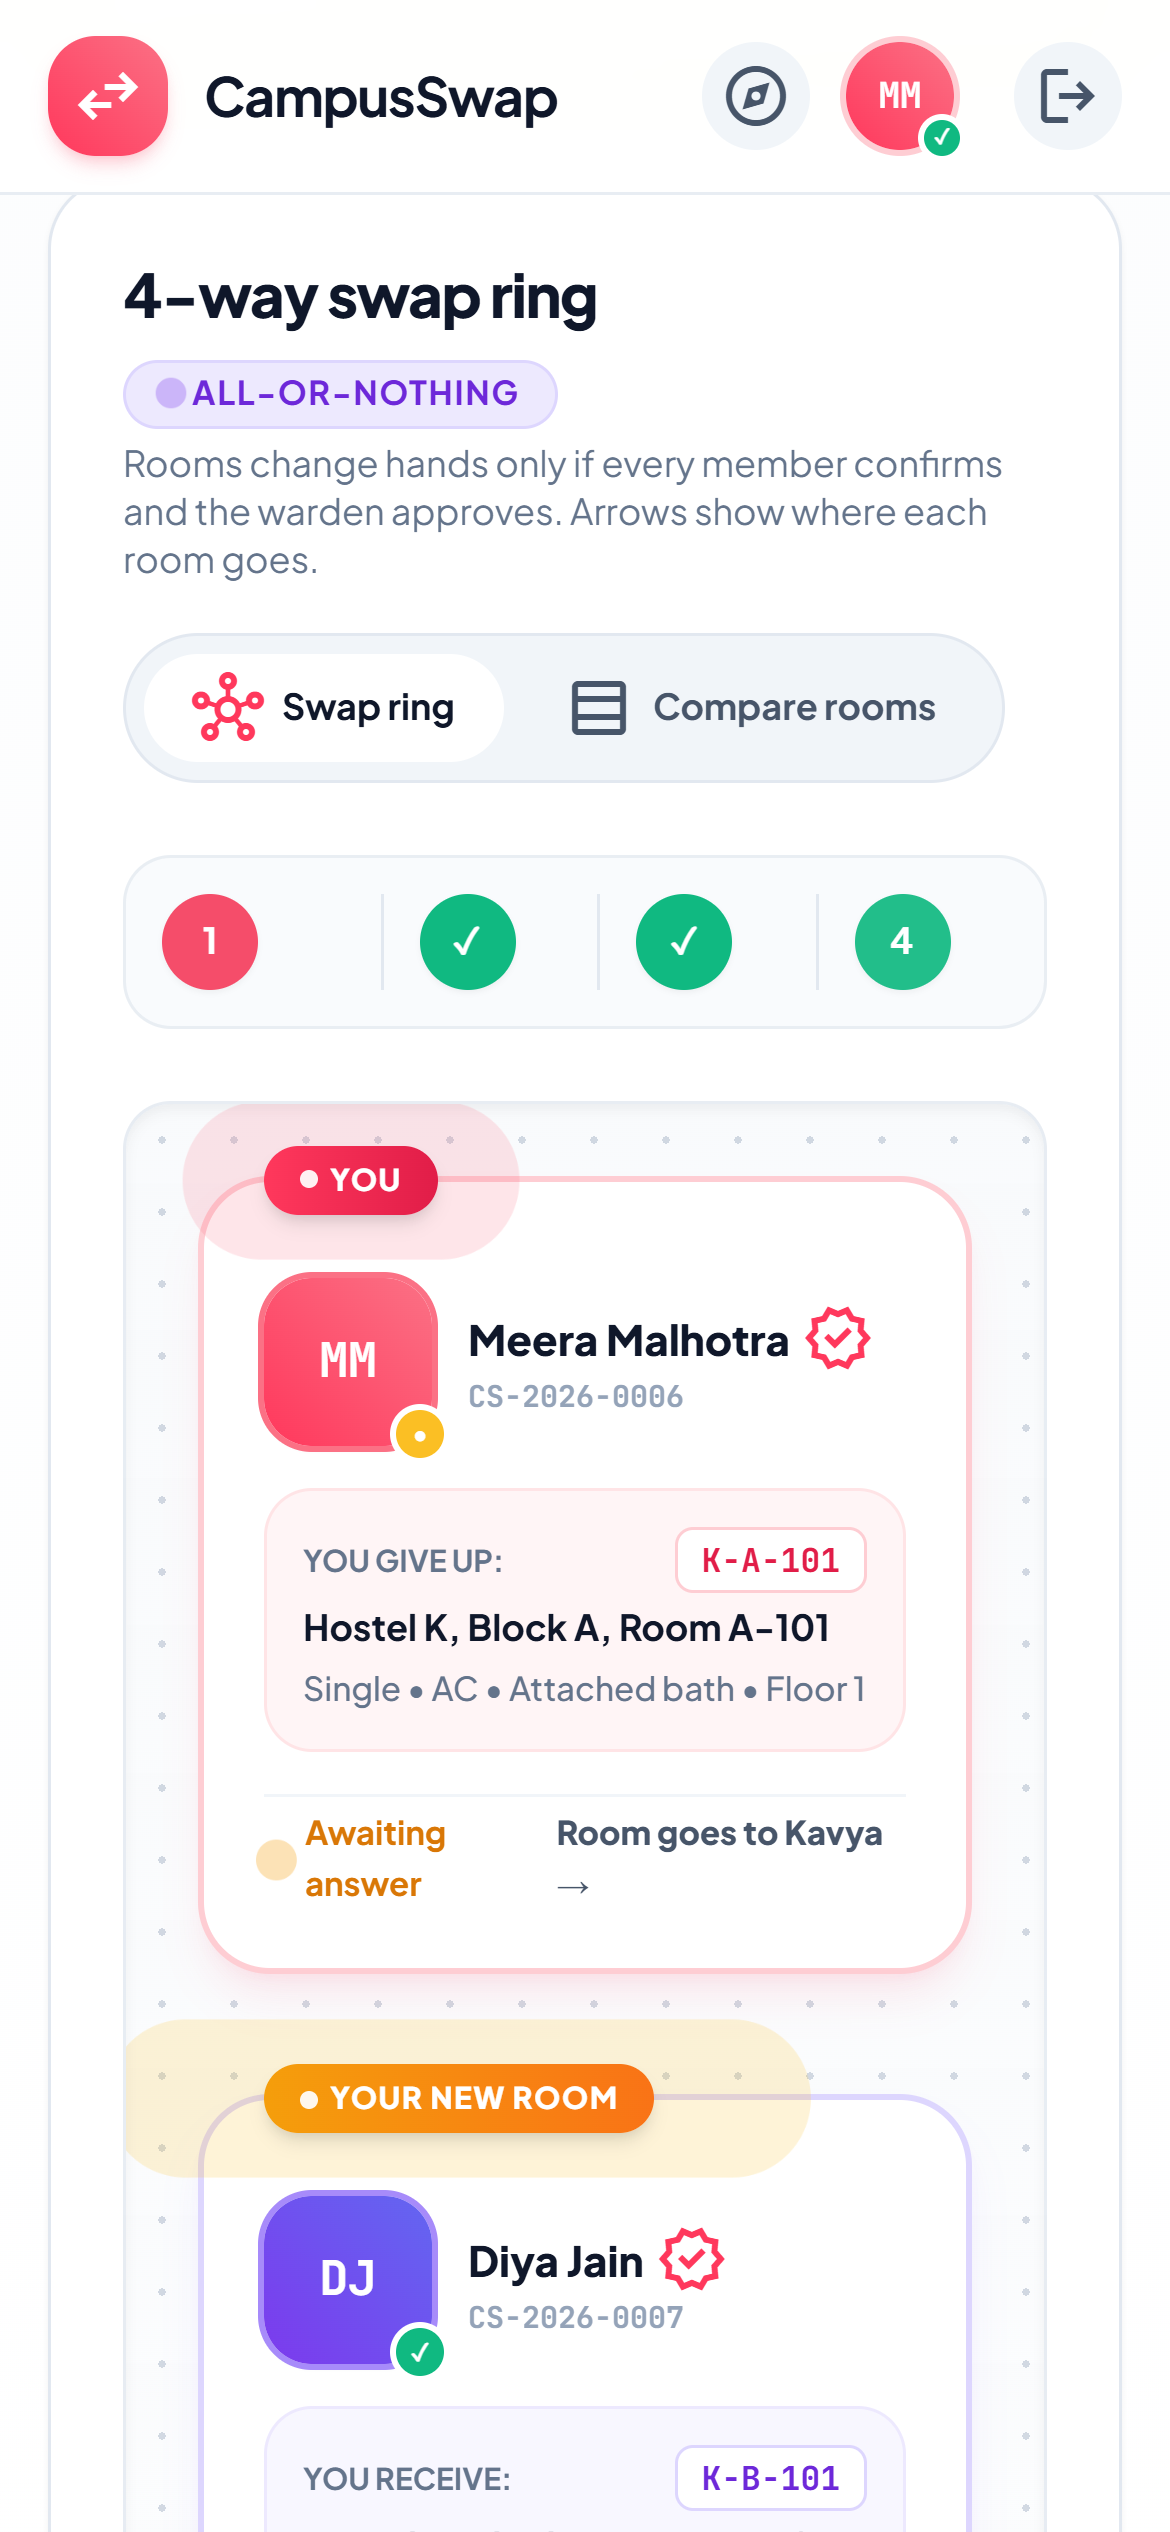
\includegraphics[width=\linewidth]{ui-ring-phone}
    \caption{The swap ring as stacked cards}
  \end{subfigure}
  \caption[Student dashboard on a phone]{The same dashboard on a phone
    screen, 390 pixels wide.}
  \label{fig:ui-phone}
\end{figure}

\begin{figure}[tbp]
  \centering
  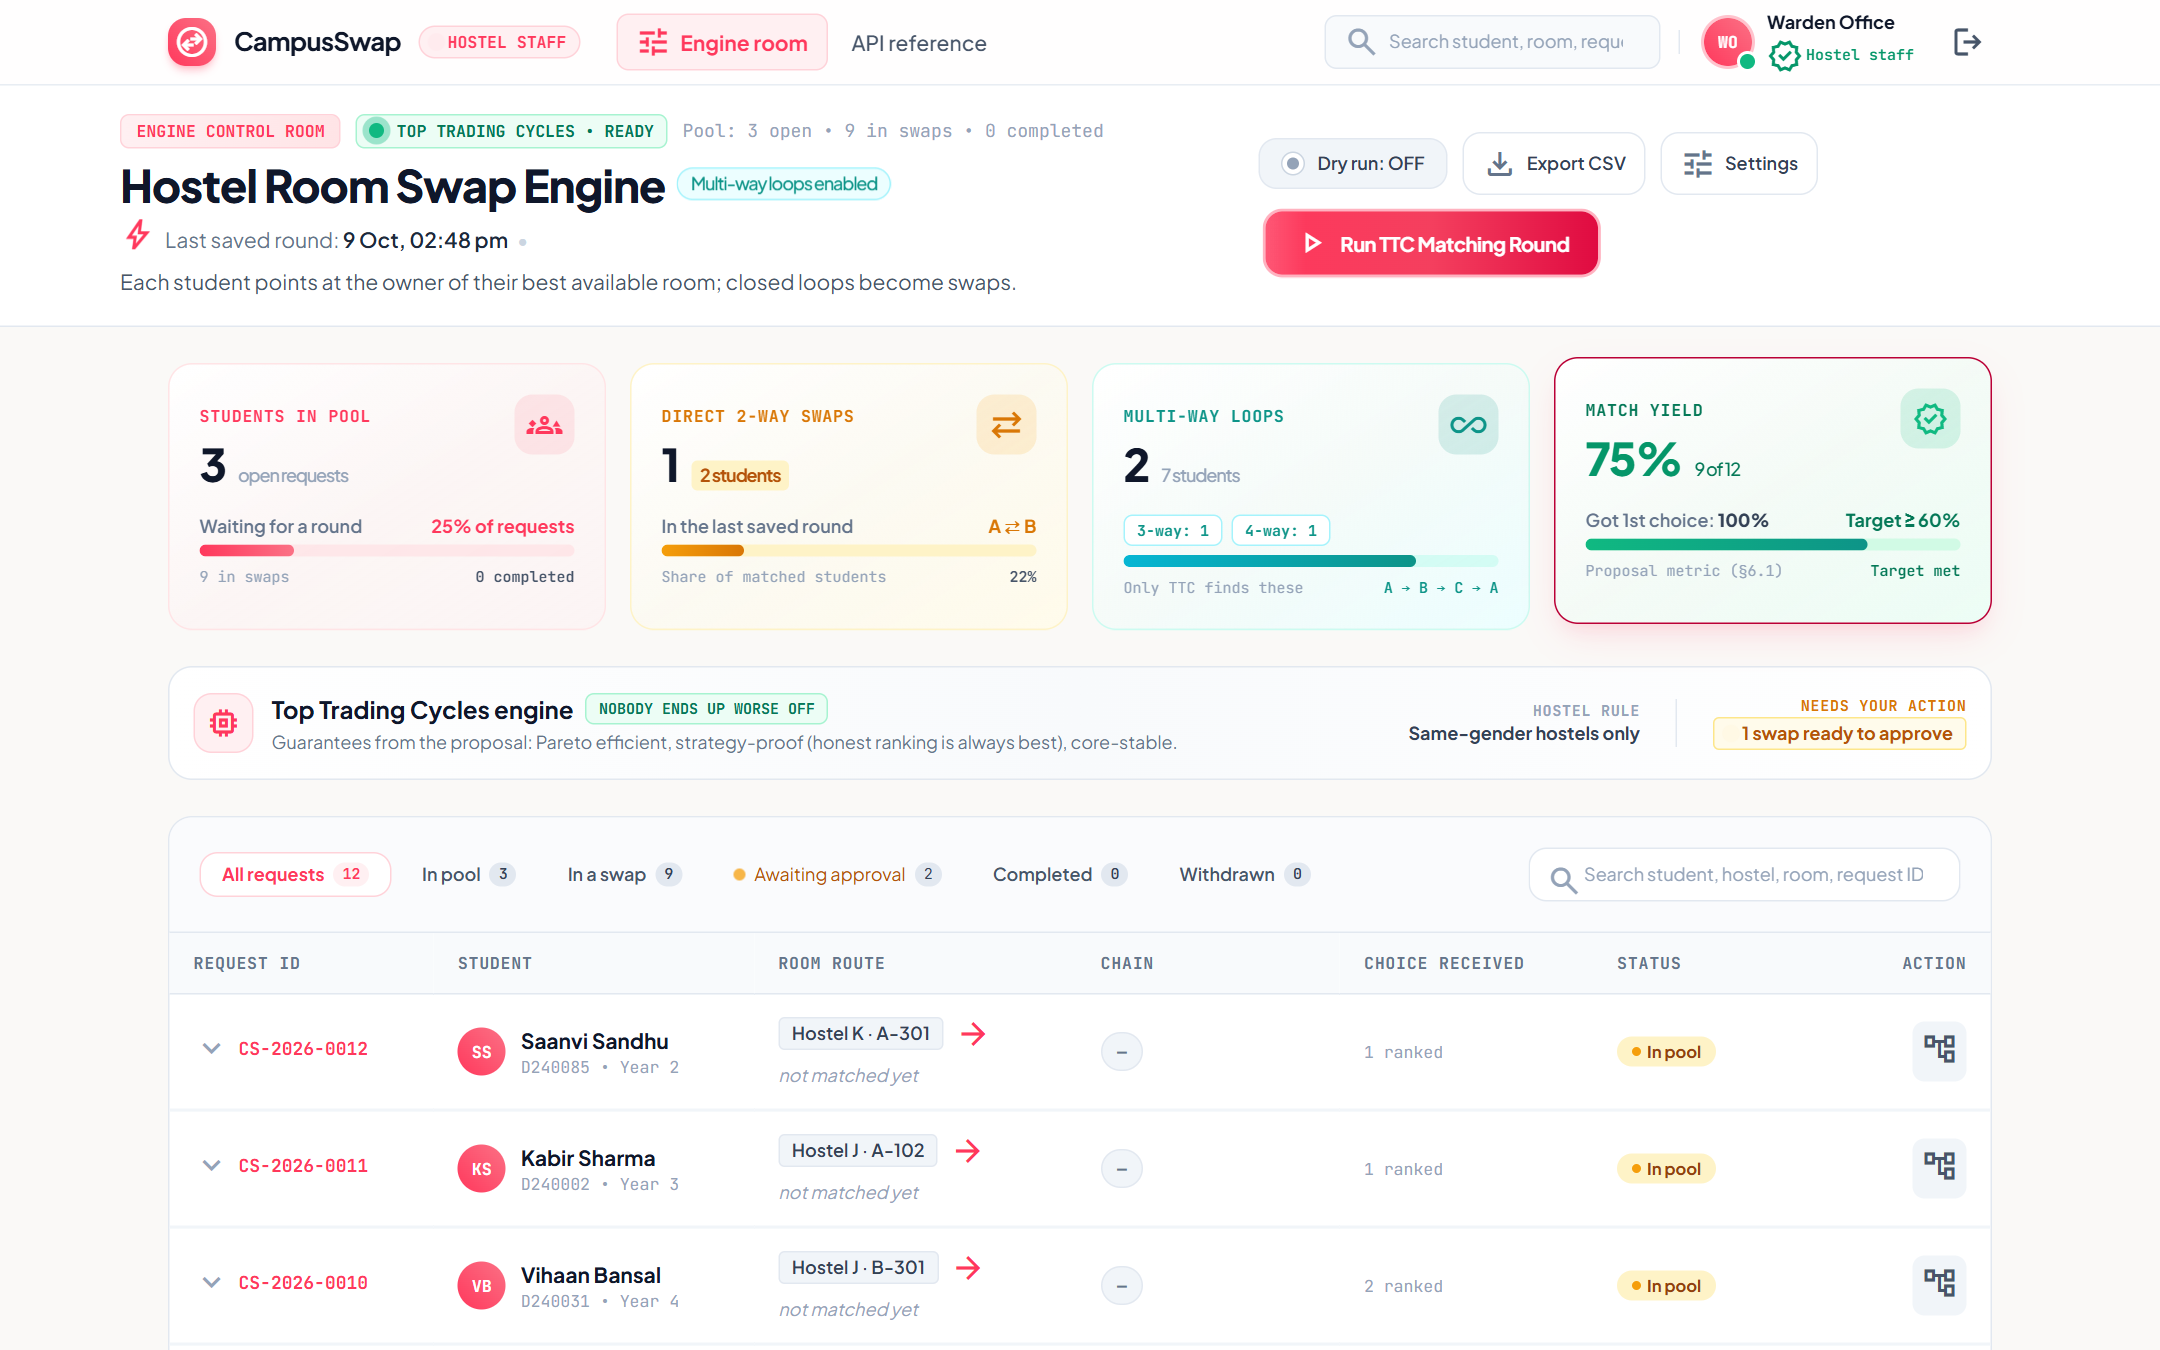
\includegraphics[width=\linewidth]{ui-admin}
  \caption[Hostel staff page]{Hostel staff page (``Engine room''): run a
    round, see the Match Yield against the 60\% target, the count of 2-way
    swaps and multi-way loops, and every request with its chain and
    status.}
  \label{fig:ui-admin}
\end{figure}

\begin{figure}[tbp]
  \centering
  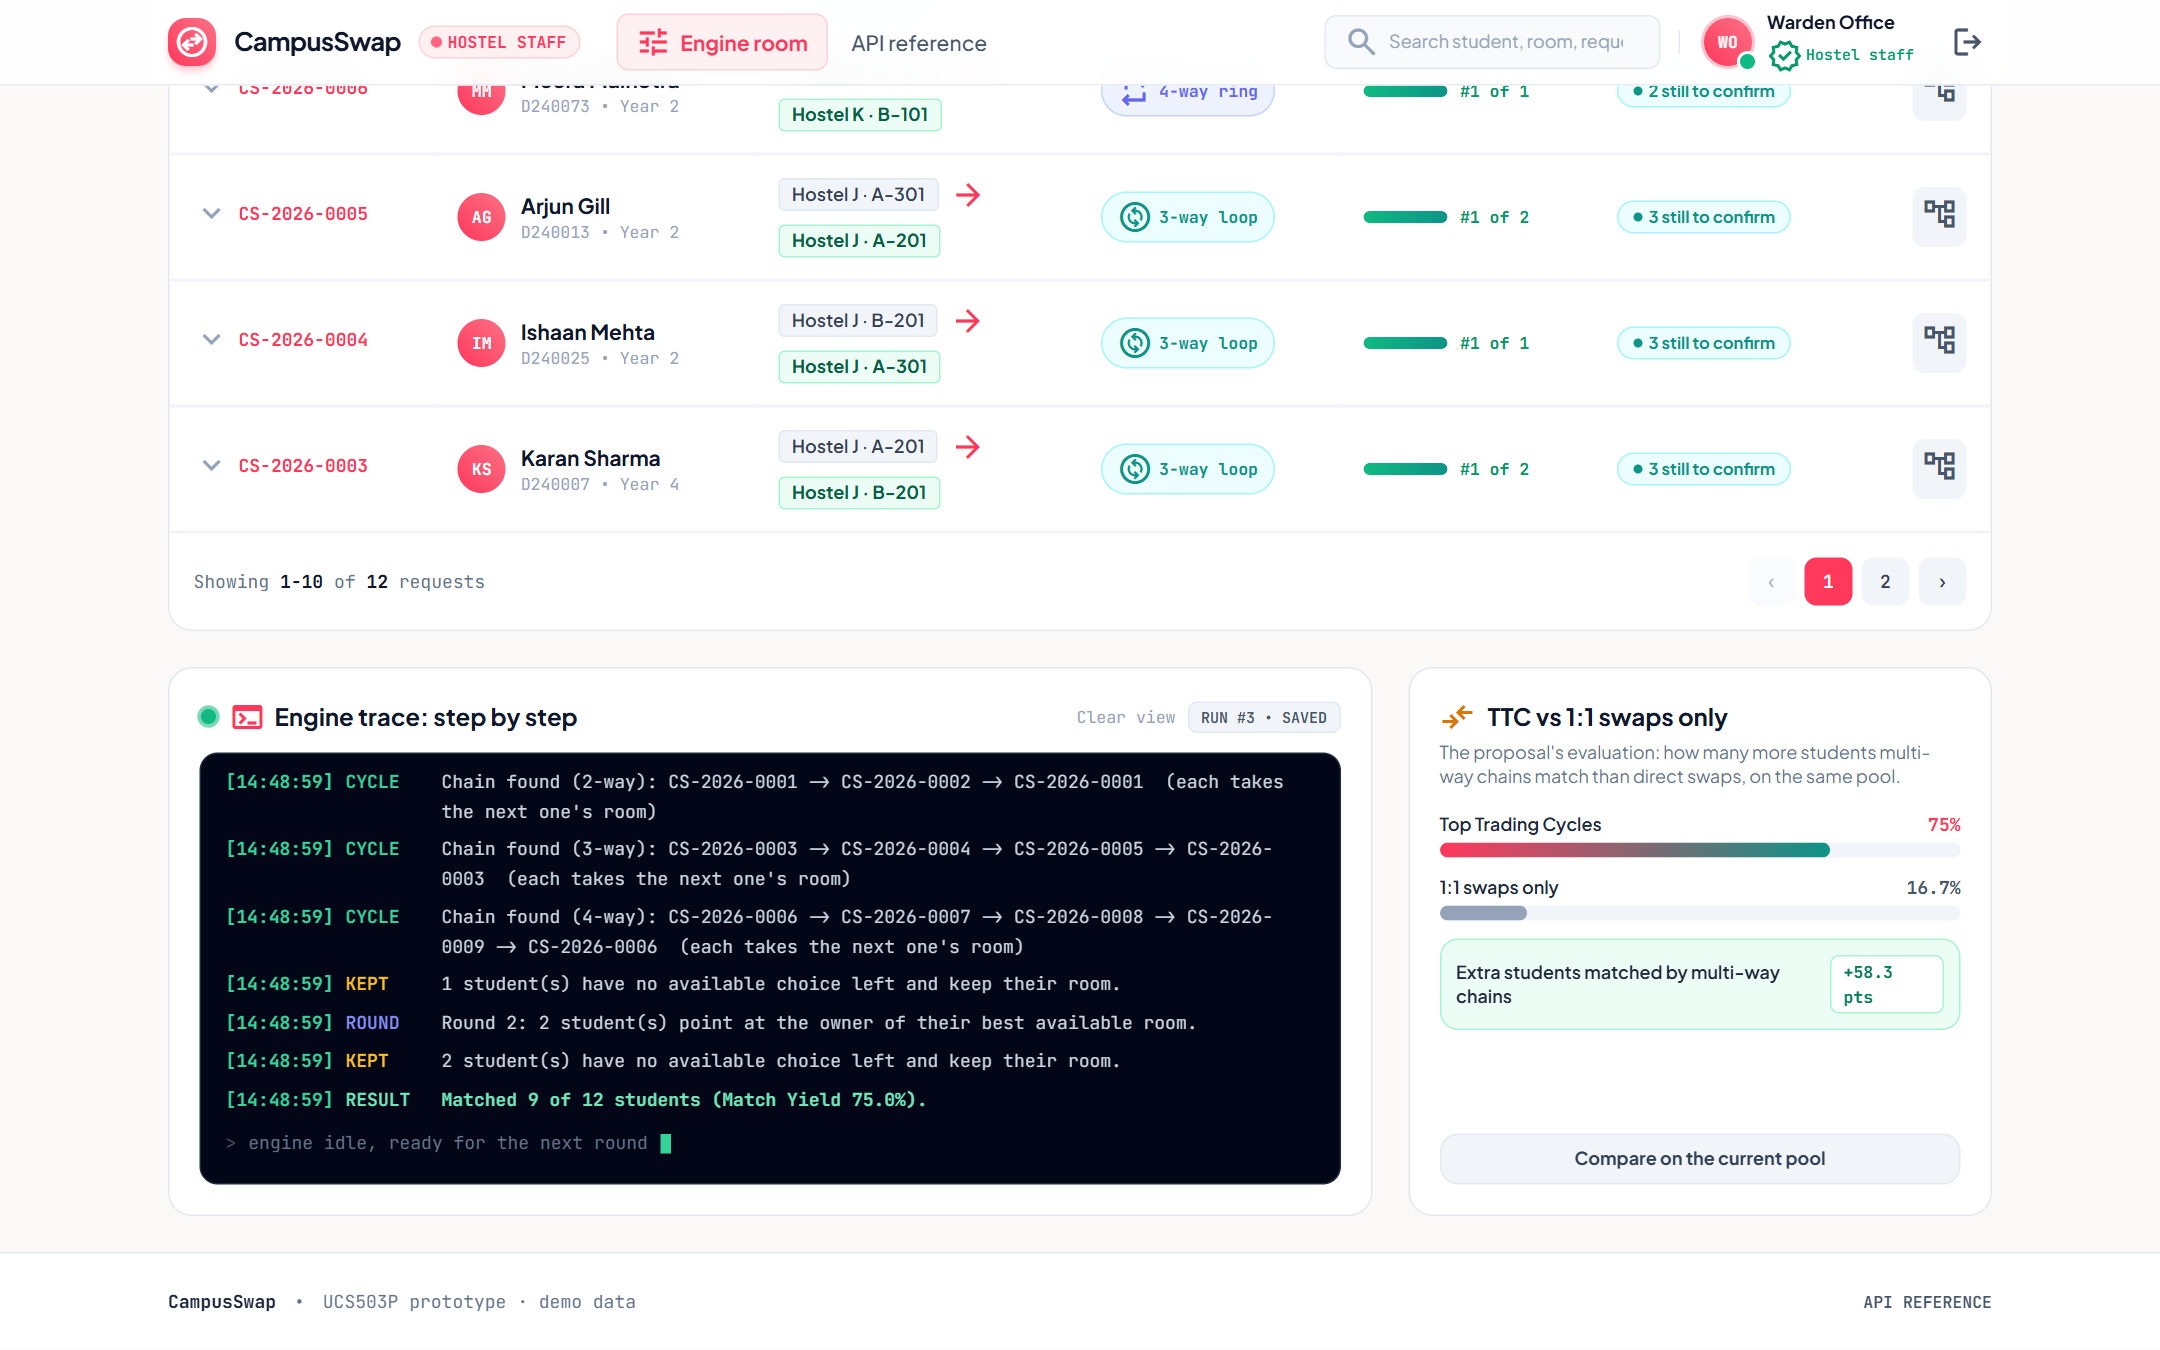
\includegraphics[width=\linewidth]{ui-trace}
  \caption[Engine trace and TTC versus one-to-one comparison]{Lower part of
    the hostel staff page: the engine's real step-by-step trace for the
    round, and the comparison on the same pool (TTC matched 75\% of
    students, direct one-to-one swaps only 16.7\%).}
  \label{fig:ui-trace}
\end{figure}

\section{Hardware Interfaces}

CampusSwap needs no special hardware. Users need a device with a web
browser. The server can be an ordinary laptop or a small cloud server; the
whole database is one file.

\section{Software Interfaces}

\subsection{Web API}

The pages talk to the server only through the JSON interface below (an
\emph{API}). All paths start with \texttt{/api}.

\begin{xltabular}{\linewidth}{@{}lL{5.5cm}L{1.9cm}Y@{}}
  \caption{Web API}\label{tab:api}\\
  \toprule
  \textbf{Method} & \textbf{Path} & \textbf{Who} & \textbf{What it does}\\
  \midrule
  \endfirsthead
  \toprule
  \textbf{Method} & \textbf{Path} & \textbf{Who} & \textbf{What it does}\\
  \midrule
  \endhead
  \bottomrule
  \endlastfoot
  POST & \texttt{/auth/login} & anyone & Body \texttt{\{email, password,
    role\}}. Sets the session cookie.\\
  POST & \texttt{/auth/logout} & anyone & Ends the session.\\
  GET & \texttt{/auth/me} & signed in & The current user.\\
  GET & \texttt{/auth/status} & anyone & The current user or
    \texttt{null}; never an error.\\
  GET & \texttt{/public/stats} & anyone & Open requests, rooms, hostels,
    requests per day for 7 days, last round. No personal data.\\
  \midrule
  GET & \texttt{/rooms} & student & Rooms in eligible hostels, with
    \texttt{is\_own} and \texttt{open\_to\_swap}.\\
  GET & \texttt{/me/dashboard} & student & Room, request, chain,
    milestones and activity.\\
  POST & \texttt{/requests} & student & Body \texttt{\{room\_ids\}}, 1--5
    rooms, best first. Returns \texttt{201} and the tracking ID.\\
  DELETE & \texttt{/requests/current} & student & Withdraw the open
    request.\\
  POST & \texttt{/cycles/\{id\}/accept} & student & Accept a place in a
    proposed chain.\\
  POST & \texttt{/cycles/\{id\}/decline} & student & Decline; the chain is
    cancelled for everyone.\\
  \midrule
  GET & \texttt{/admin/overview} & staff & Counts, latest round, latest
    comparison, latest trace.\\
  GET & \texttt{/admin/requests} & staff & Every request with its chain.\\
  POST & \texttt{/admin/match-runs} & staff & Body \texttt{\{algorithm,
    dry\_run\}}. Runs a round.\\
  POST & \texttt{/admin/compare} & staff & Dry-runs TTC and one-to-one
    swaps on the same pool.\\
  POST & \texttt{/admin/cycles/\{id\}/approve} & staff & Approve a confirmed
    chain; seats change hands.\\
  GET & \texttt{/admin/export.csv} & staff & Download all requests as
    \texttt{campusswap-requests.csv}.\\
\end{xltabular}

Every error has the same shape, so a page can always show a clear
message:
\begin{lstlisting}
{"error": "own_room", "message": "You can't rank the room you already live in."}
\end{lstlisting}

\begin{xltabular}{\linewidth}{@{}lL{4.2cm}Y@{}}
  \caption{Error responses}\label{tab:errors}\\
  \toprule
  \textbf{Status} & \textbf{Meaning} & \textbf{Error codes}\\
  \midrule
  \endfirsthead
  \toprule
  \textbf{Status} & \textbf{Meaning} & \textbf{Error codes}\\
  \midrule
  \endhead
  \bottomrule
  \endlastfoot
  400 & The request breaks a rule & \texttt{empty\_list}, \texttt{too\_many},
    \texttt{duplicate\_room}, \texttt{own\_room}, \texttt{unknown\_room},
    \texttt{wrong\_hostel\_gender}, \texttt{unknown\_algorithm},
    \texttt{pairwise\_must\_be\_dry\_run}\\
  401 & Not signed in, or wrong password & \texttt{not\_logged\_in},
    \texttt{bad\_credentials}\\
  403 & Signed in, but not allowed & \texttt{forbidden}, \texttt{wrong\_role},
    \texttt{not\_member}\\
  404 & Does not exist & \texttt{no\_request}, \texttt{no\_cycle}\\
  409 & Not possible right now & \texttt{already\_active}, \texttt{in\_cycle},
    \texttt{no\_seat}, \texttt{cycle\_closed}, \texttt{already\_answered},
    \texttt{not\_confirmed}, \texttt{run\_in\_progress}\\
  422 & The body has the wrong shape & \texttt{invalid\_input}\\
\end{xltabular}

\subsection{Internal interfaces}

\begin{itemize}
  \item \textbf{Server and database:} SQLAlchemy 2.0 over SQLite, with
    foreign keys switched on. Times are stored in UTC.
  \item \textbf{Server and matching engine:} plain Python function calls.
    The server passes a list of participants (each with an ID, the seat
    they own and the seats they want, best first) to
    \texttt{top\_trading\_cycles()} and receives the chains, who gets which
    seat, who keeps their seat, and a round-by-round record.
\end{itemize}

\section{Communications Interfaces}

\begin{itemize}
  \item Browser and server communicate over HTTP, with JSON bodies in
    UTF-8.
  \item After sign-in the browser holds a session cookie,
    \texttt{cs\_session}. It is marked \emph{HttpOnly} (page scripts cannot
    read it) and \emph{SameSite=Lax} (other websites cannot send it in
    form posts), and expires after 12 hours.
  \item For a real deployment the server shall be reached only over HTTPS,
    with the cookie also marked \emph{Secure} (\Req{NFR-SEC-07},
    \Built: \texttt{run.py --cert --key}).
  \item Members of a chain are emailed when it is found and before the
    deadline (\Req{FR-CONF-06}, \Built; sent only when a mail server is set up).
\end{itemize}

% ======================================================================
\chapter{System Features}\label{ch:features}
% ======================================================================

CampusSwap is a room-swap system. Its core is collecting ranked requests
and finding fair chains of swaps; everything else supports that.

\section{Description and Priority}

The features, from most to least important:

\begin{enumerate}
  \item \textbf{Run a matching round} (High). The reason the system
    exists: it finds the swap chains.
  \item \textbf{Submit and withdraw a swap request} (High). Without
    requests there is nothing to match.
  \item \textbf{Accept or decline a swap chain} (High). Nobody is moved
    without agreeing.
  \item \textbf{Approve a chain} (High). The warden's final check before
    rooms change.
  \item \textbf{Sign in and sessions} (High). Keeps each user to their own
    actions.
  \item \textbf{Browse rooms} (Medium). Helps students choose; a student
    could rank rooms without it.
  \item \textbf{Status tracking and reports} (Medium). Builds trust and
    gives the hostel office its records.
  \item \textbf{Faculty slot exchange} (Low). Reuses the same
    engine for lecture slots.
\end{enumerate}

The sequence diagram in Section~\ref{sec:design}
(Figure~\ref{fig:sequence}) shows how the main features work together for
one swap, from the student's request to the warden's approval.

\section{Functional Requirements}

% ---------------------------------------------------------------- AUTH
\subsection{Sign in and sessions}

\paragraph{Description and priority.} Users sign in with an email address,
a password and a role (Student or Hostel Staff). Priority: High.

\paragraph{Stimulus and response.}
\begin{enumerate}
  \item The user enters an email and password and presses \emph{Sign in}.
    The system checks them and opens the right home page, or shows
    ``Wrong email or password.''
  \item The user presses \emph{Sign out}. The system ends the session and
    returns to the sign-in page.
\end{enumerate}

\begin{xltabular}{\linewidth}{@{}L{2.25cm}YL{1.55cm}L{1.6cm}@{}}
  \caption{Requirements: sign in and sessions}\label{tab:fr-auth}\\
  \ReqHeader
  \endfirsthead
  \ReqHeader
  \endhead
  \bottomrule
  \endlastfoot
  \Req{FR-AUTH-01} & The system shall let a user sign in with an email
    address, a password and a role (Student, Hostel Staff or Faculty). & High &
    \Built\\
  \Req{FR-AUTH-02} & The system shall ignore letter case and surrounding
    spaces in the email address. & Medium & \Built\\
  \Req{FR-AUTH-03} & For an unknown email or a wrong password, the system
    shall give the same answer (\texttt{401 bad\_credentials}) and take
    about the same time, so nobody can find out which accounts exist. &
    High & \Built\\
  \Req{FR-AUTH-04} & If the password is right but the user chose the
    wrong role tab, the system shall say which tab to use
    (\texttt{403 wrong\_role}). & Medium & \Built\\
  \Req{FR-AUTH-05} & On sign-in the system shall start a session that
    lasts 12 hours, held in the \texttt{cs\_session} cookie. & High &
    \Built\\
  \Req{FR-AUTH-06} & Signing out shall delete the session on the server and
    clear the cookie. & High & \Built\\
  \Req{FR-AUTH-07} & Every student action shall require a signed-in
    student, and every staff action a signed-in staff member
    (otherwise \texttt{401 not\_logged\_in} or \texttt{403 forbidden}). &
    High & \Built\\
  \Req{FR-AUTH-08} & The sign-in page shall accept only addresses ending in
    \texttt{@thapar.edu}. & Medium & \Built\\
  \Req{FR-AUTH-09} & The server shall also refuse sign-in for addresses
    outside \texttt{@thapar.edu} (not only the page). &
    Medium & \Built\\
  \Req{FR-AUTH-10} & The system shall slow down or block repeated failed
    sign-in attempts. & Medium & \Built\\
  \Req{FR-AUTH-11} & Students shall be able to sign in with the
    institute's Microsoft account (single sign-on). & Low & \Planned\\
\end{xltabular}

% ---------------------------------------------------------------- ROOM
\subsection{Browse rooms}

\paragraph{Description and priority.} A student sees every room they could
move to and picks the ones to rank. Priority: Medium.

\paragraph{Stimulus and response.}
\begin{enumerate}
  \item The student opens \emph{Explore Rooms}. The system lists every room
    in the hostels of the student's gender.
  \item The student changes a filter or types a search. The list updates
    at once.
  \item The student presses \emph{Rank in Preferences} on a room. The room
    joins the ranked list on the right.
\end{enumerate}

\begin{xltabular}{\linewidth}{@{}L{2.25cm}YL{1.55cm}L{1.6cm}@{}}
  \caption{Requirements: browse rooms}\label{tab:fr-room}\\
  \ReqHeader
  \endfirsthead
  \ReqHeader
  \endhead
  \bottomrule
  \endlastfoot
  \Req{FR-ROOM-01} & The system shall show a student only the rooms in
    hostels that house the student's gender. & High & \Built\\
  \Req{FR-ROOM-02} & For each room the system shall show the hostel,
    block, floor, room number, number of beds (1--3), air conditioning,
    washroom type (attached or common) and tags. & High & \Built\\
  \Req{FR-ROOM-03} & For each room the system shall show how many of its
    other occupants have an open request (``open to swap''), without
    showing their names. & Medium & \Built\\
  \Req{FR-ROOM-04} & The system shall mark the student's own room and not
    let it be ranked. & High & \Built\\
  \Req{FR-ROOM-05} & The page shall filter by hostel, floor, number of
    beds, air conditioning, attached washroom and ``someone wants to
    swap'', and search by hostel, block or room number. & Medium &
    \Built\\
  \Req{FR-ROOM-06} & The page shall offer a detailed view and a compact
    view, split into pages. & Low & \Built\\
  \Req{FR-ROOM-07} & A student shall be able to rank a room type (for
    example ``any single AC room on floor 1'') instead of one specific
    room. & Low & \Built\\
\end{xltabular}

% ---------------------------------------------------------------- REQ
\subsection{Submit and withdraw a swap request}

\paragraph{Description and priority.} A student turns their ranked list
into a swap request, or takes it back. Priority: High.

\paragraph{Stimulus and response.}
\begin{enumerate}
  \item The student presses \emph{Submit}. If the list breaks a rule, the
    system shows the reason and saves nothing. Otherwise it saves the
    request as \emph{open} and shows its tracking ID.
  \item The student presses \emph{Withdraw}. If the request is still open,
    the system marks it \emph{withdrawn}.
\end{enumerate}

\begin{xltabular}{\linewidth}{@{}L{2.25cm}YL{1.55cm}L{1.6cm}@{}}
  \caption{Requirements: submit and withdraw a swap request}\label{tab:fr-req}\\
  \ReqHeader
  \endfirsthead
  \ReqHeader
  \endhead
  \bottomrule
  \endlastfoot
  \Req{FR-REQ-01} & A student shall be able to rank one to five rooms, best
    first, and submit them as one request. & High & \Built\\
  \Req{FR-REQ-02} & Before submitting, the student shall be able to
    reorder the list by dragging (desktop) or with up and down buttons
    (any screen), and remove rooms. & Medium & \Built\\
  \Req{FR-REQ-03} & The system shall refuse an empty list
    (\texttt{empty\_list}), more than five rooms (\texttt{too\_many}) and
    the same room twice (\texttt{duplicate\_room}). & High & \Built\\
  \Req{FR-REQ-04} & The system shall refuse a request from a student who
    has no seat (\texttt{no\_seat}) or who already has an open or matched
    request (\texttt{already\_active}). & High & \Built\\
  \Req{FR-REQ-05} & The system shall refuse a room that does not exist
    (\texttt{unknown\_room}), the student's own room (\texttt{own\_room}) and
    a room in a hostel for the other gender
    (\texttt{wrong\_hostel\_gender}). & High & \Built\\
  \Req{FR-REQ-06} & A valid request shall be saved as \emph{open}, together
    with its ranked rooms and the seat the student offers, and given a
    tracking ID of the form \texttt{CS-YYYY-NNNN} (year, then a four-digit
    number). & High & \Built\\
  \Req{FR-REQ-07} & A student shall be able to withdraw a request only
    while it is open. A matched request cannot be withdrawn
    (\texttt{in\_cycle}); the student declines the chain instead. & High &
    \Built\\
  \Req{FR-REQ-08} & Every submit and withdraw shall be recorded in the
    event log. & Medium & \Built\\
\end{xltabular}

% ---------------------------------------------------------------- MATCH
\subsection{Run a matching round}

\paragraph{Description and priority.} Hostel staff run Top Trading Cycles
over every open request and save the chains it finds. Priority: High.

\paragraph{How Top Trading Cycles works.} Every student in the pool owns a
seat and wants some rooms, best first. Repeat until nobody is left:
\begin{enumerate}
  \item Each remaining student points at the owner of their best room that
    is still available. A student with no choice left points at
    themselves.
  \item Every closed loop of pointers is a chain: each member takes the
    seat of the person they point at. A student pointing at themselves
    keeps their room.
  \item Everyone in a loop is removed, together with their seats.
\end{enumerate}
Because every student points at exactly one person, at least one loop
always exists, so the method always finishes. TTC is known to give an
outcome that no other assignment can improve for someone without hurting
someone else, in which nobody gains by ranking dishonestly, and from which
no group can break away and do better among themselves
[\ref{ref:shapley}, \ref{ref:roth82}].

\paragraph{Stimulus and response.}
\begin{enumerate}
  \item Staff press \emph{Run TTC Matching Round}. The system dissolves
    overdue chains, runs TTC on the pool, saves the chains, and shows the
    Match Yield and the step-by-step trace.
  \item Staff press \emph{Compare on the current pool}. The system runs TTC
    and direct one-to-one swaps as dry runs and shows both results side by
    side.
\end{enumerate}

\begin{xltabular}{\linewidth}{@{}L{2.25cm}YL{1.55cm}L{1.6cm}@{}}
  \caption{Requirements: run a matching round}\label{tab:fr-match}\\
  \ReqHeader
  \endfirsthead
  \ReqHeader
  \endhead
  \bottomrule
  \endlastfoot
  \Req{FR-MATCH-01} & Hostel staff shall be able to run a TTC round over
    every open request (the pool). & High & \Built\\
  \Req{FR-MATCH-02} & Before building the pool, the system shall dissolve
    every proposed chain whose deadline has passed. & High & \Built\\
  \Req{FR-MATCH-03} & In a room with several beds, the system shall offer
    the beds of pool members in a fixed order (lowest seat number first),
    so the same pool always gives the same result. & High & \Built\\
  \Req{FR-MATCH-04} & The system shall never assign a student a room they
    did not rank; a student with no possible swap keeps their room. & High
    & \Built\\
  \Req{FR-MATCH-05} & A saved round shall turn each loop of two or more
    students into a \emph{proposed} chain with a deadline 48 hours after
    the round, and mark their requests \emph{matched}. & High & \Built\\
  \Req{FR-MATCH-06} & A dry run shall compute and record the round's
    numbers but create no chains and change no request. & Medium &
    \Built\\
  \Req{FR-MATCH-07} & For each round the system shall report the pool size,
    the number matched, the Match Yield (matched $\div$ pool $\times$ 100,
    one decimal place), the share of matched students who got their first
    choice, the number of chains of each length, and a plain-language
    step-by-step trace. & High & \Built\\
  \Req{FR-MATCH-08} & Only one round shall run at a time; a second attempt
    gets \texttt{409 run\_in\_progress}. & High & \Built\\
  \Req{FR-MATCH-09} & The system shall compare TTC with direct one-to-one
    swaps on the same pool at the same moment. One-to-one swaps shall only
    ever run as a dry run (\texttt{pairwise\_must\_be\_dry\_run}). & Medium
    & \Built\\
  \Req{FR-MATCH-10} & Rounds shall run automatically on a schedule set by
    the hostel office. & Low & \Built\\
\end{xltabular}

% ---------------------------------------------------------------- CONF
\subsection{Accept or decline a swap chain}

\paragraph{Description and priority.} Every member of a proposed chain
must agree before anyone moves. One ``no'' cancels the whole chain.
Priority: High.

\paragraph{Stimulus and response.}
\begin{enumerate}
  \item A member presses \emph{Confirm}. The system records the answer.
    When the last member confirms, the chain becomes \emph{confirmed} and
    waits for the warden.
  \item A member presses \emph{Decline}. The chain is dissolved at once.
    The decliner's request is withdrawn; everyone else goes back to the
    pool for the next round.
  \item The deadline passes. At the next round or answer, the chain is
    dissolved. Members who did not answer are withdrawn; members who
    accepted go back to the pool.
\end{enumerate}

\begin{xltabular}{\linewidth}{@{}L{2.25cm}YL{1.55cm}L{1.6cm}@{}}
  \caption{Requirements: accept or decline a swap chain}\label{tab:fr-conf}\\
  \ReqHeader
  \endfirsthead
  \ReqHeader
  \endhead
  \bottomrule
  \endlastfoot
  \Req{FR-CONF-01} & The system shall show each member the whole chain: who
    gives which room, who has answered, which choice the member receives,
    and the time left before the deadline. & High & \Built\\
  \Req{FR-CONF-02} & A member shall be able to accept once. When every
    member has accepted, the chain shall become \emph{confirmed}. & High &
    \Built\\
  \Req{FR-CONF-03} & A member shall be able to decline. The chain shall be
    dissolved, the decliner's request withdrawn, and every other member's
    request put back to \emph{open}. & High & \Built\\
  \Req{FR-CONF-04} & A proposed chain whose deadline has passed shall be
    dissolved when the next round runs or any member answers. Members who
    did not answer are withdrawn; members who accepted go back to
    \emph{open}. & High & \Built\\
  \Req{FR-CONF-05} & The system shall refuse an answer from a non-member
    (\texttt{not\_member}), for a chain that is no longer proposed
    (\texttt{cycle\_closed}), or from a member who already answered
    (\texttt{already\_answered}). & High & \Built\\
  \Req{FR-CONF-06} & The system shall email each member when a chain is
    found and again before the deadline. & Medium & \Built\\
\end{xltabular}

% ---------------------------------------------------------------- APPR
\subsection{Approve a chain}

\paragraph{Description and priority.} The warden gives the final approval;
only then do rooms change. Priority: High.

\paragraph{Stimulus and response.} The warden presses \emph{Approve} on a
confirmed chain. The system moves each member to the seat they receive and
marks their requests \emph{completed}.

\begin{xltabular}{\linewidth}{@{}L{2.25cm}YL{1.55cm}L{1.6cm}@{}}
  \caption{Requirements: approve a chain}\label{tab:fr-appr}\\
  \ReqHeader
  \endfirsthead
  \ReqHeader
  \endhead
  \bottomrule
  \endlastfoot
  \Req{FR-APPR-01} & Hostel staff shall be able to approve only a chain in
    which every member has accepted (otherwise \texttt{409
    not\_confirmed}). & High & \Built\\
  \Req{FR-APPR-02} & On approval, in one database transaction, every member
    shall move to the seat they receive, their requests become
    \emph{completed}, and the chain becomes \emph{approved}. & High &
    \Built\\
  \Req{FR-APPR-03} & The system shall produce a signed-off approval form
    (PDF) listing every member, for the hostel office. & Medium &
    \Built\\
\end{xltabular}

% ---------------------------------------------------------------- TRACK
\subsection{Status tracking and reports}

\paragraph{Description and priority.} Students always know where their
request stands; staff always have a complete record. Priority: Medium.

\paragraph{Stimulus and response.} A student opens the dashboard and sees
their room, request and chain. Staff open the engine room and see every
request; pressing \emph{Export CSV} downloads them as a spreadsheet.

\begin{xltabular}{\linewidth}{@{}L{2.25cm}YL{1.55cm}L{1.6cm}@{}}
  \caption{Requirements: status tracking and reports}\label{tab:fr-track}\\
  \ReqHeader
  \endfirsthead
  \ReqHeader
  \endhead
  \bottomrule
  \endlastfoot
  \Req{FR-TRACK-01} & The student dashboard shall show the current room,
    the active request and its tracking ID, the chain (if any), and five
    milestones: Request submitted, In the matching pool, Match found,
    Everyone confirmed, Warden approved. & High & \Built\\
  \Req{FR-TRACK-02} & The dashboard shall list the last 20 events about
    the student, newest first. & Medium & \Built\\
  \Req{FR-TRACK-03} & The dashboard shall explain what to do next when
    the student has no request, is waiting in the pool, or was not matched.
    & Medium & \Built\\
  \Req{FR-TRACK-04} & The staff overview shall show the number of open,
    matched and completed requests, the chains waiting for approval, the
    latest saved round, the latest comparison, the latest trace, and the
    Match Yield of the last ten saved rounds. & High & \Built\\
  \Req{FR-TRACK-05} & The staff request table shall show every request
    with the student's name, roll number and year, the room offered, the
    ranked rooms, the room assigned, the choice received, and the chain
    with each member's answer; it shall be searchable and filterable by
    status. & High & \Built\\
  \Req{FR-TRACK-06} & Staff shall be able to download all requests as
    \texttt{campusswap-requests.csv} with the columns \texttt{tracking\_id},
    \texttt{student}, \texttt{roll\_no}, \texttt{status},
    \texttt{offered\_room}, \texttt{assigned\_room},
    \texttt{received\_rank}, \texttt{cycle\_id}, \texttt{cycle\_length},
    \texttt{cycle\_status}, \texttt{submitted\_at}. & Medium & \Built\\
  \Req{FR-TRACK-07} & The sign-in page shall show public numbers (open
    requests, rooms, hostels, requests per day for the last seven days,
    last round) without any personal data. & Low & \Built\\
  \Req{FR-TRACK-08} & Staff shall be able to download the full event log
    as an audit trail. & Medium & \Built\\
\end{xltabular}

% ---------------------------------------------------------------- SLOT
\subsection{Faculty slot exchange}

\paragraph{Description and priority.} Faculty members swap lecture slots
using the same engine: each owns a slot and ranks slots they prefer.
Priority: Low.

\begin{xltabular}{\linewidth}{@{}L{2.25cm}YL{1.55cm}L{1.6cm}@{}}
  \caption{Requirements: faculty slot exchange}\label{tab:fr-slot}\\
  \ReqHeader
  \endfirsthead
  \ReqHeader
  \endhead
  \bottomrule
  \endlastfoot
  \Req{FR-SLOT-01} & Faculty shall be able to rank lecture slots they would
    prefer to their own, and the matching engine shall find slot-swap
    chains in the same way as for rooms. & Low & \Built\\
\end{xltabular}

% ======================================================================
\chapter{Other Nonfunctional Requirements}
% ======================================================================

\section{Performance Requirements}

\begin{xltabular}{\linewidth}{@{}L{2.25cm}YL{1.55cm}L{1.6cm}@{}}
  \caption{Performance requirements}\label{tab:nfr-perf}\\
  \ReqHeader
  \endfirsthead
  \ReqHeader
  \endhead
  \bottomrule
  \endlastfoot
  \Req{NFR-PERF-01} & The matching step for a pool of 2{,}000 requests shall
    take less than 2 seconds. An automated test checks this; on the team's
    laptop it took 17~ms (median of five runs). & High & \Built\\
  \Req{NFR-PERF-02} & The time for a round shall grow at most with the
    square of the pool size: each student's pointer only moves forward
    through their own list. & Medium & \Built\\
  \Req{NFR-PERF-03} & The pages shall be usable on a phone screen 390 pixels
    wide without sideways scrolling. & High & \Built\\
  \Req{NFR-PERF-04} & The pages shall load and work with no internet
    access (fonts, icons and styles are stored locally). & Medium &
    \Built\\
\end{xltabular}

\section{Safety Requirements}

Here, safety means protecting data from being lost, mixed up or exposed.

\begin{xltabular}{\linewidth}{@{}L{2.25cm}YL{1.55cm}L{1.6cm}@{}}
  \caption{Safety requirements}\label{tab:nfr-safe}\\
  \ReqHeader
  \endfirsthead
  \ReqHeader
  \endhead
  \bottomrule
  \endlastfoot
  \Req{NFR-SAFE-01} & Every change shall happen inside one database
    transaction: a matching round or an approval is saved completely or
    not at all. & High & \Built\\
  \Req{NFR-SAFE-02} & The database shall make it impossible for two
    students to occupy the same seat (a unique rule on the seat's
    occupant). & High & \Built\\
  \Req{NFR-SAFE-03} & The database shall reject any row that points at
    something that does not exist (foreign keys switched on). & High &
    \Built\\
  \Req{NFR-SAFE-04} & A request shall not rank the same room twice or use
    the same rank twice (unique rules in the database). & High & \Built\\
  \Req{NFR-SAFE-05} & The prototype shall contain only made-up data. & High
    & \Built\\
  \Req{NFR-SAFE-06} & Students' names shall not be shown while browsing
    rooms; they are shown only to members of the same chain and to hostel
    staff. & High & \Built\\
\end{xltabular}

\section{Security Requirements}

\begin{xltabular}{\linewidth}{@{}L{2.25cm}YL{1.55cm}L{1.6cm}@{}}
  \caption{Security requirements}\label{tab:nfr-sec}\\
  \ReqHeader
  \endfirsthead
  \ReqHeader
  \endhead
  \bottomrule
  \endlastfoot
  \Req{NFR-SEC-01} & Passwords shall never be stored as plain text. The
    system stores a salted \emph{scrypt} hash ($N=2^{14}$, $r=8$, $p=1$,
    16-byte random salt) and compares hashes in constant time. & High &
    \Built\\
  \Req{NFR-SEC-02} & A session token shall be 32 random bytes. The server
    shall store only its SHA-256 hash, so a leaked database cannot be used
    to sign in. & High & \Built\\
  \Req{NFR-SEC-03} & The session cookie shall be HttpOnly and SameSite=Lax,
    and expire after 12 hours. & High & \Built\\
  \Req{NFR-SEC-04} & The server shall check the user's role on every
    request; hiding a button on the page is never the only protection. &
    High & \Built\\
  \Req{NFR-SEC-05} & All text that came from users shall be escaped before
    it is put on a page, so nobody can inject their own script. & High &
    \Built\\
  \Req{NFR-SEC-06} & Error messages shall not reveal whether an email
    address has an account. & Medium & \Built\\
  \Req{NFR-SEC-07} & A deployed system shall be reached only over HTTPS,
    with the cookie marked Secure. & High & \Built\\
  \Req{NFR-SEC-08} & Repeated failed sign-ins shall be limited (see
    \Req{FR-AUTH-10}). & Medium & \Built\\
\end{xltabular}

\section{Software Quality Attributes}

\begin{itemize}
  \item \textbf{Correctness and testability.} 89 automated tests check the
    engine, every business rule and the web API (Appendix~\ref{app:trace}).
    The engine is tested with made-up participants and no database,
    including 50 random pools of 40 students in which nobody is ever
    given a seat they did not ask for.
  \item \textbf{Reliability.} GitHub Actions runs every test on each push
    and pull request, so a change that breaks a rule is caught before it
    is merged.
  \item \textbf{Maintainability.} Each rule lives in one place (the
    services layer). Pages never repeat a rule; they only show the server's
    answer.
  \item \textbf{Portability.} The server runs on Windows, Linux and macOS.
    Moving from SQLite to PostgreSQL needs only a different database
    address.
  \item \textbf{Usability.} Plain-language messages, a demo-accounts hint
    on the sign-in page, and the loading, empty and error states described
    in Section~\ref{sec:ui}.
  \item \textbf{Explainability.} Every round produces a plain-language
    trace (``Chain found (3-way): \ldots''), so staff and students can see
    why a chain was proposed.
\end{itemize}

\needspace{10\baselineskip}
\section{Business Rules}\label{sec:rules}

\begin{xltabular}{\linewidth}{@{}L{1.4cm}Y@{}}
  \caption{Business rules}\label{tab:rules}\\
  \toprule
  \textbf{ID} & \textbf{Rule}\\
  \midrule
  \endfirsthead
  \toprule
  \textbf{ID} & \textbf{Rule}\\
  \midrule
  \endhead
  \bottomrule
  \endlastfoot
  \Req{BR-01} & A student may only rank rooms in hostels that house their
    own gender.\\
  \Req{BR-02} & A request ranks one to five different rooms, never the
    student's own room.\\
  \Req{BR-03} & A student has at most one active (open or matched) request
    at a time.\\
  \Req{BR-04} & Only an open request may be withdrawn.\\
  \Req{BR-05} & Only hostel staff may run rounds, compare methods, approve
    chains and export records.\\
  \Req{BR-06} & Every member of a chain must accept within 48 hours of the
    round.\\
  \Req{BR-07} & A chain is all-or-nothing: one decline cancels it for
    everyone.\\
  \Req{BR-08} & Rooms change only after the warden approves a confirmed
    chain.\\
  \Req{BR-09} & Nobody is ever moved to a room they did not rank; a student
    with no swap keeps their room.\\
  \Req{BR-10} & CampusSwap's approval is a record for the hostel office,
    which still updates its own master allotment records.\\
  \Req{BR-11} & A one-to-one comparison never changes any request or
    room.\\
\end{xltabular}

% ======================================================================
\chapter{Other Requirements}
% ======================================================================

\section{Maintenance}

CampusSwap will be used for many semesters, so it must stay easy to
change.
\begin{itemize}
  \item Every new rule shall come with an automated test, and the full
    test suite shall pass before a change is merged.
  \item Diagrams are kept as text (PlantUML) next to the code, and redrawn
    with \texttt{python} \path{diagrams/render.py}, so they can be updated with
    the code.
  \item The matching engine shall stay free of database and web code, so it
    can be reused (for example, for faculty slot exchange).
\end{itemize}

\section{Data and privacy}

\begin{itemize}
  \item The system shall collect only what matching needs: name, roll
    number, gender, year, branch, current seat and ranked rooms.
  \item Before a pilot with real students (planned with 20 to 40
    volunteers), each participant shall give consent, and the data shall
    be deleted after the pilot.
  \item Sessions expire after 12 hours; expired sessions can be removed at
    any time without losing any other data.
\end{itemize}

\section{Deployment (Phase~2)}

\begin{itemize}
  \item The system shall run on a server reachable only over HTTPS
    (\Req{NFR-SEC-07}).
  \item For many users at once, the database shall move to PostgreSQL.
  \item Long rounds, notifications and deadline checks may move to a
    background worker if pools become very large.
\end{itemize}

% ======================================================================
\appendix
% ======================================================================

\chapter{Glossary}\label{app:glossary}

\begin{xltabular}{\linewidth}{@{}L{3.5cm}Y@{}}
  \toprule
  \textbf{Term} & \textbf{Meaning}\\
  \midrule
  \endfirsthead
  \toprule
  \textbf{Term} & \textbf{Meaning}\\
  \midrule
  \endhead
  \bottomrule
  \endlastfoot
  API & Application Programming Interface: the fixed set of requests the
    pages can send to the server.\\
  Chain (cycle) & A closed loop of students in which each takes the next
    one's seat. A 2-way chain is a direct swap.\\
  Core-stable & No group of students can leave the result and swap among
    themselves so that all of them do better.\\
  CSV & Comma-separated values: a plain spreadsheet file.\\
  Data flow diagram (DFD) & A picture of where data comes from, which
    process changes it and where it is stored.\\
  Dry run & A round that is calculated and reported but changes nothing.\\
  ER diagram & Entity--relationship diagram: the database tables and how
    they link.\\
  Hash & A one-way scrambled form of a secret. The original cannot be
    worked out from it.\\
  HTTP / HTTPS & The language browsers and servers use to talk. HTTPS is
    the encrypted version.\\
  HttpOnly cookie & A cookie that page scripts cannot read, so injected
    code cannot steal it.\\
  JSON & A simple text format for sending structured data.\\
  Match Yield & Students placed in a chain $\div$ students in the pool
    $\times$ 100.\\
  Pareto efficient & No other assignment makes someone happier without
    making someone else unhappier.\\
  Pool & All open requests at the moment a round runs.\\
  Scrypt & A deliberately slow password-hashing method, so stolen hashes
    are hard to crack.\\
  Seat & One bed in a room. A double room has two seats, each with its
    own occupant.\\
  Session & The server's memory that a browser has signed in.\\
  SHA-256 & A standard hash function.\\
  Single sign-on (SSO) & Signing in with an existing institute account
    instead of a separate password.\\
  SQLite & A database stored in a single file.\\
  Strategy-proof & Ranking rooms honestly is always a student's best
    move.\\
  Top Trading Cycles (TTC) & The matching method CampusSwap uses (Shapley
    and Scarf, 1974).\\
  Tracking ID & The request's public ID, for example
    \texttt{CS-2026-0013}.\\
  Warden & Hostel staff member who runs rounds and approves swaps.\\
\end{xltabular}

\chapter{Analysis Models}\label{app:models}

The diagrams already shown in this document are the context diagram
(Figure~\ref{fig:context}), architecture (Figure~\ref{fig:architecture}),
use case diagram (Figure~\ref{fig:usecase}), Level~1 data flow diagram
(Figure~\ref{fig:dfd1}), activity diagram (Figure~\ref{fig:activity}),
state diagrams (Figures~\ref{fig:state-request} and
\ref{fig:state-cycle}) and sequence diagram (Figure~\ref{fig:sequence}).
This appendix adds the class diagram, drawn in two parts so that each
stays readable, and the ER diagram.

\begin{figure}[tbp]
  \centering
  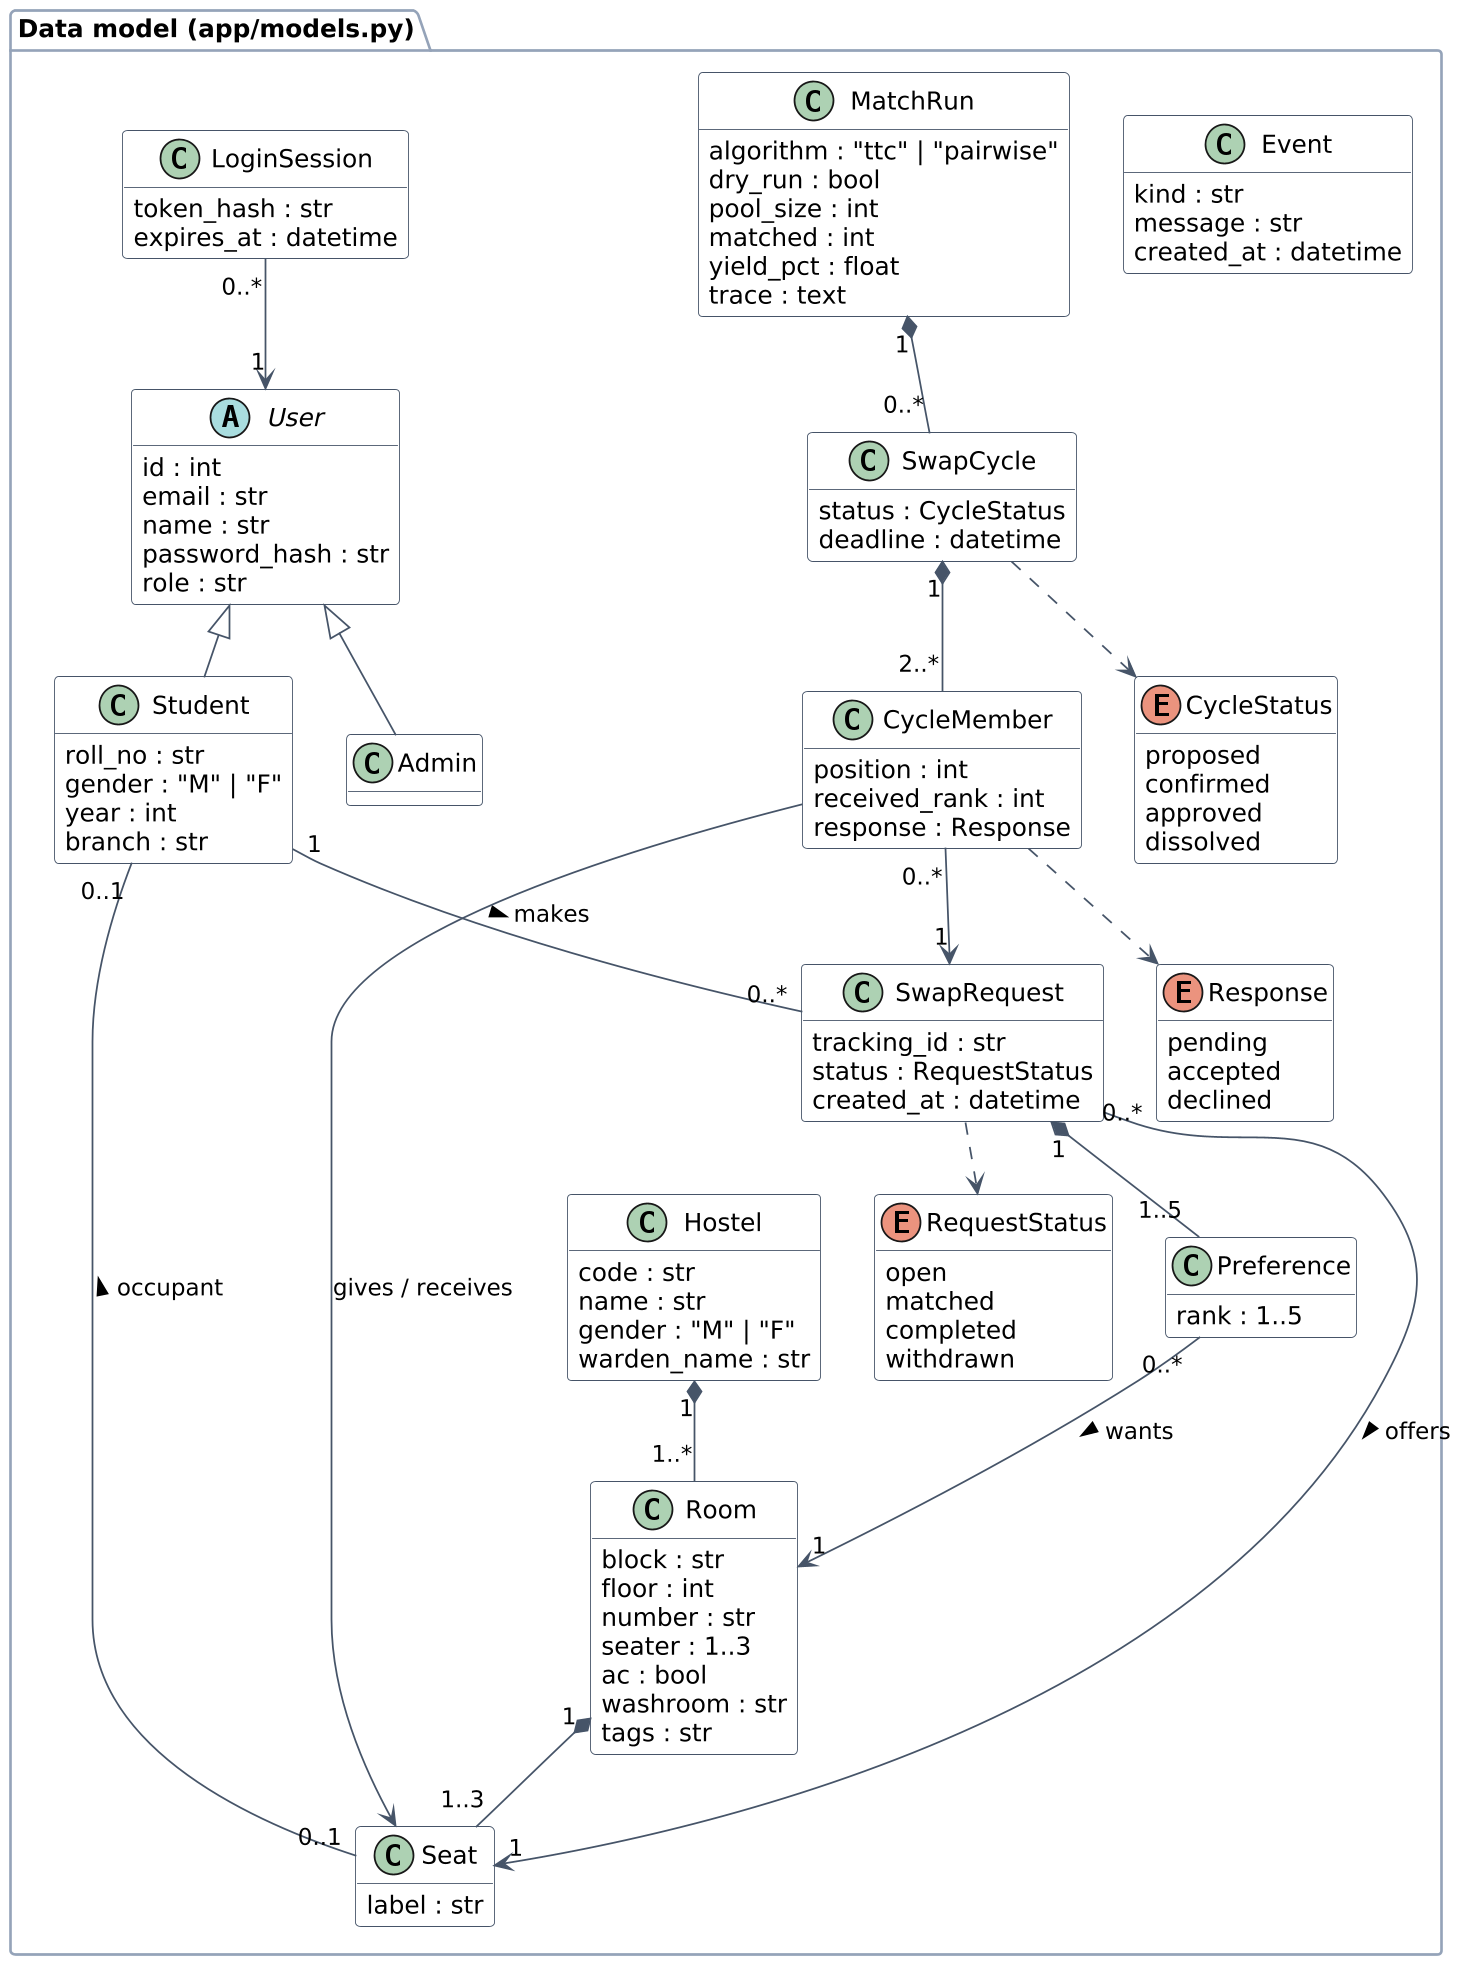
\includegraphics[width=\linewidth,height=0.88\textheight,keepaspectratio]{class}
  \caption[Class diagram, part 1: domain model]{Class diagram, part 1: the
    domain model. Student and Admin inherit from User (hollow triangle); a
    filled diamond means the part cannot exist without its whole (a room
    without its hostel, a seat without its room).}
  \label{fig:class}
\end{figure}

\begin{figure}[tbp]
  \centering
  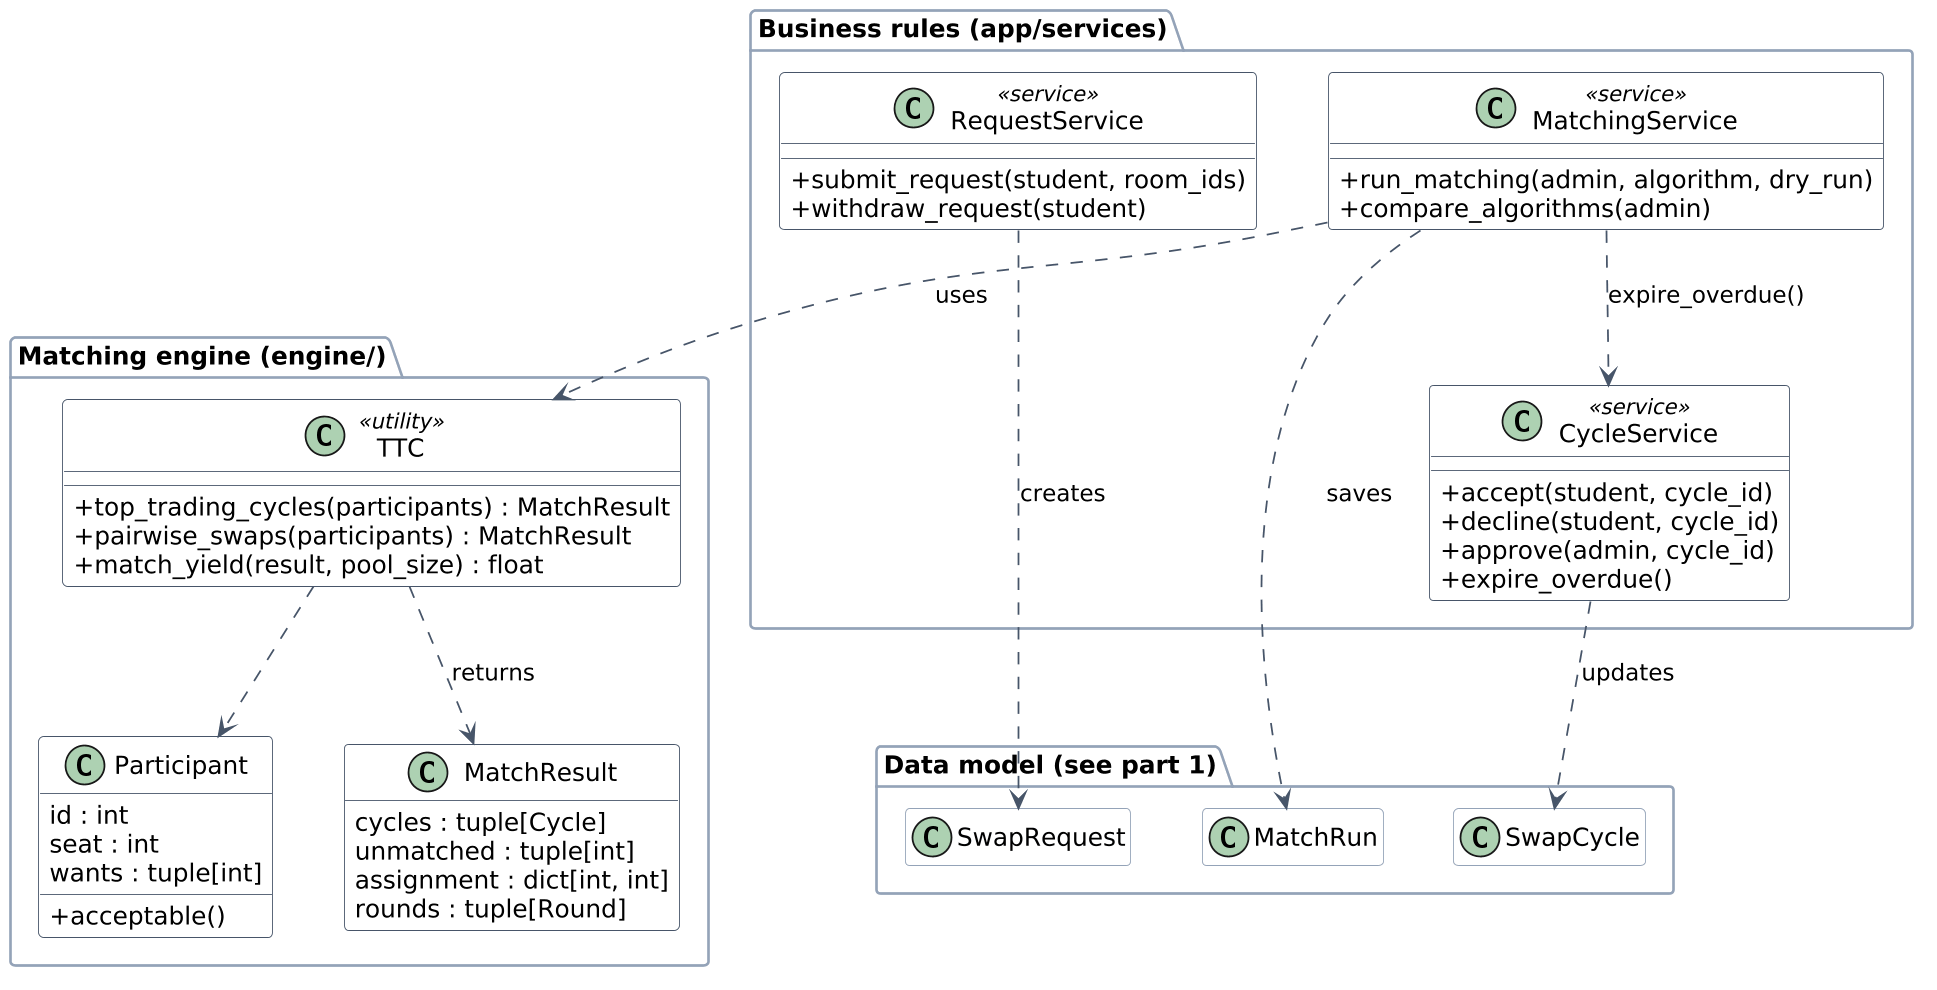
\includegraphics[width=\linewidth]{class-services}
  \caption[Class diagram, part 2: services and matching engine]{Class
    diagram, part 2: the services that hold the business rules, and the
    matching engine. Dashed arrows are dependencies: a class uses another
    without storing it. The three data classes are shown by name only;
    their attributes are in part~1.}
  \label{fig:class-services}
\end{figure}

\begin{figure}[tbp]
  \centering
  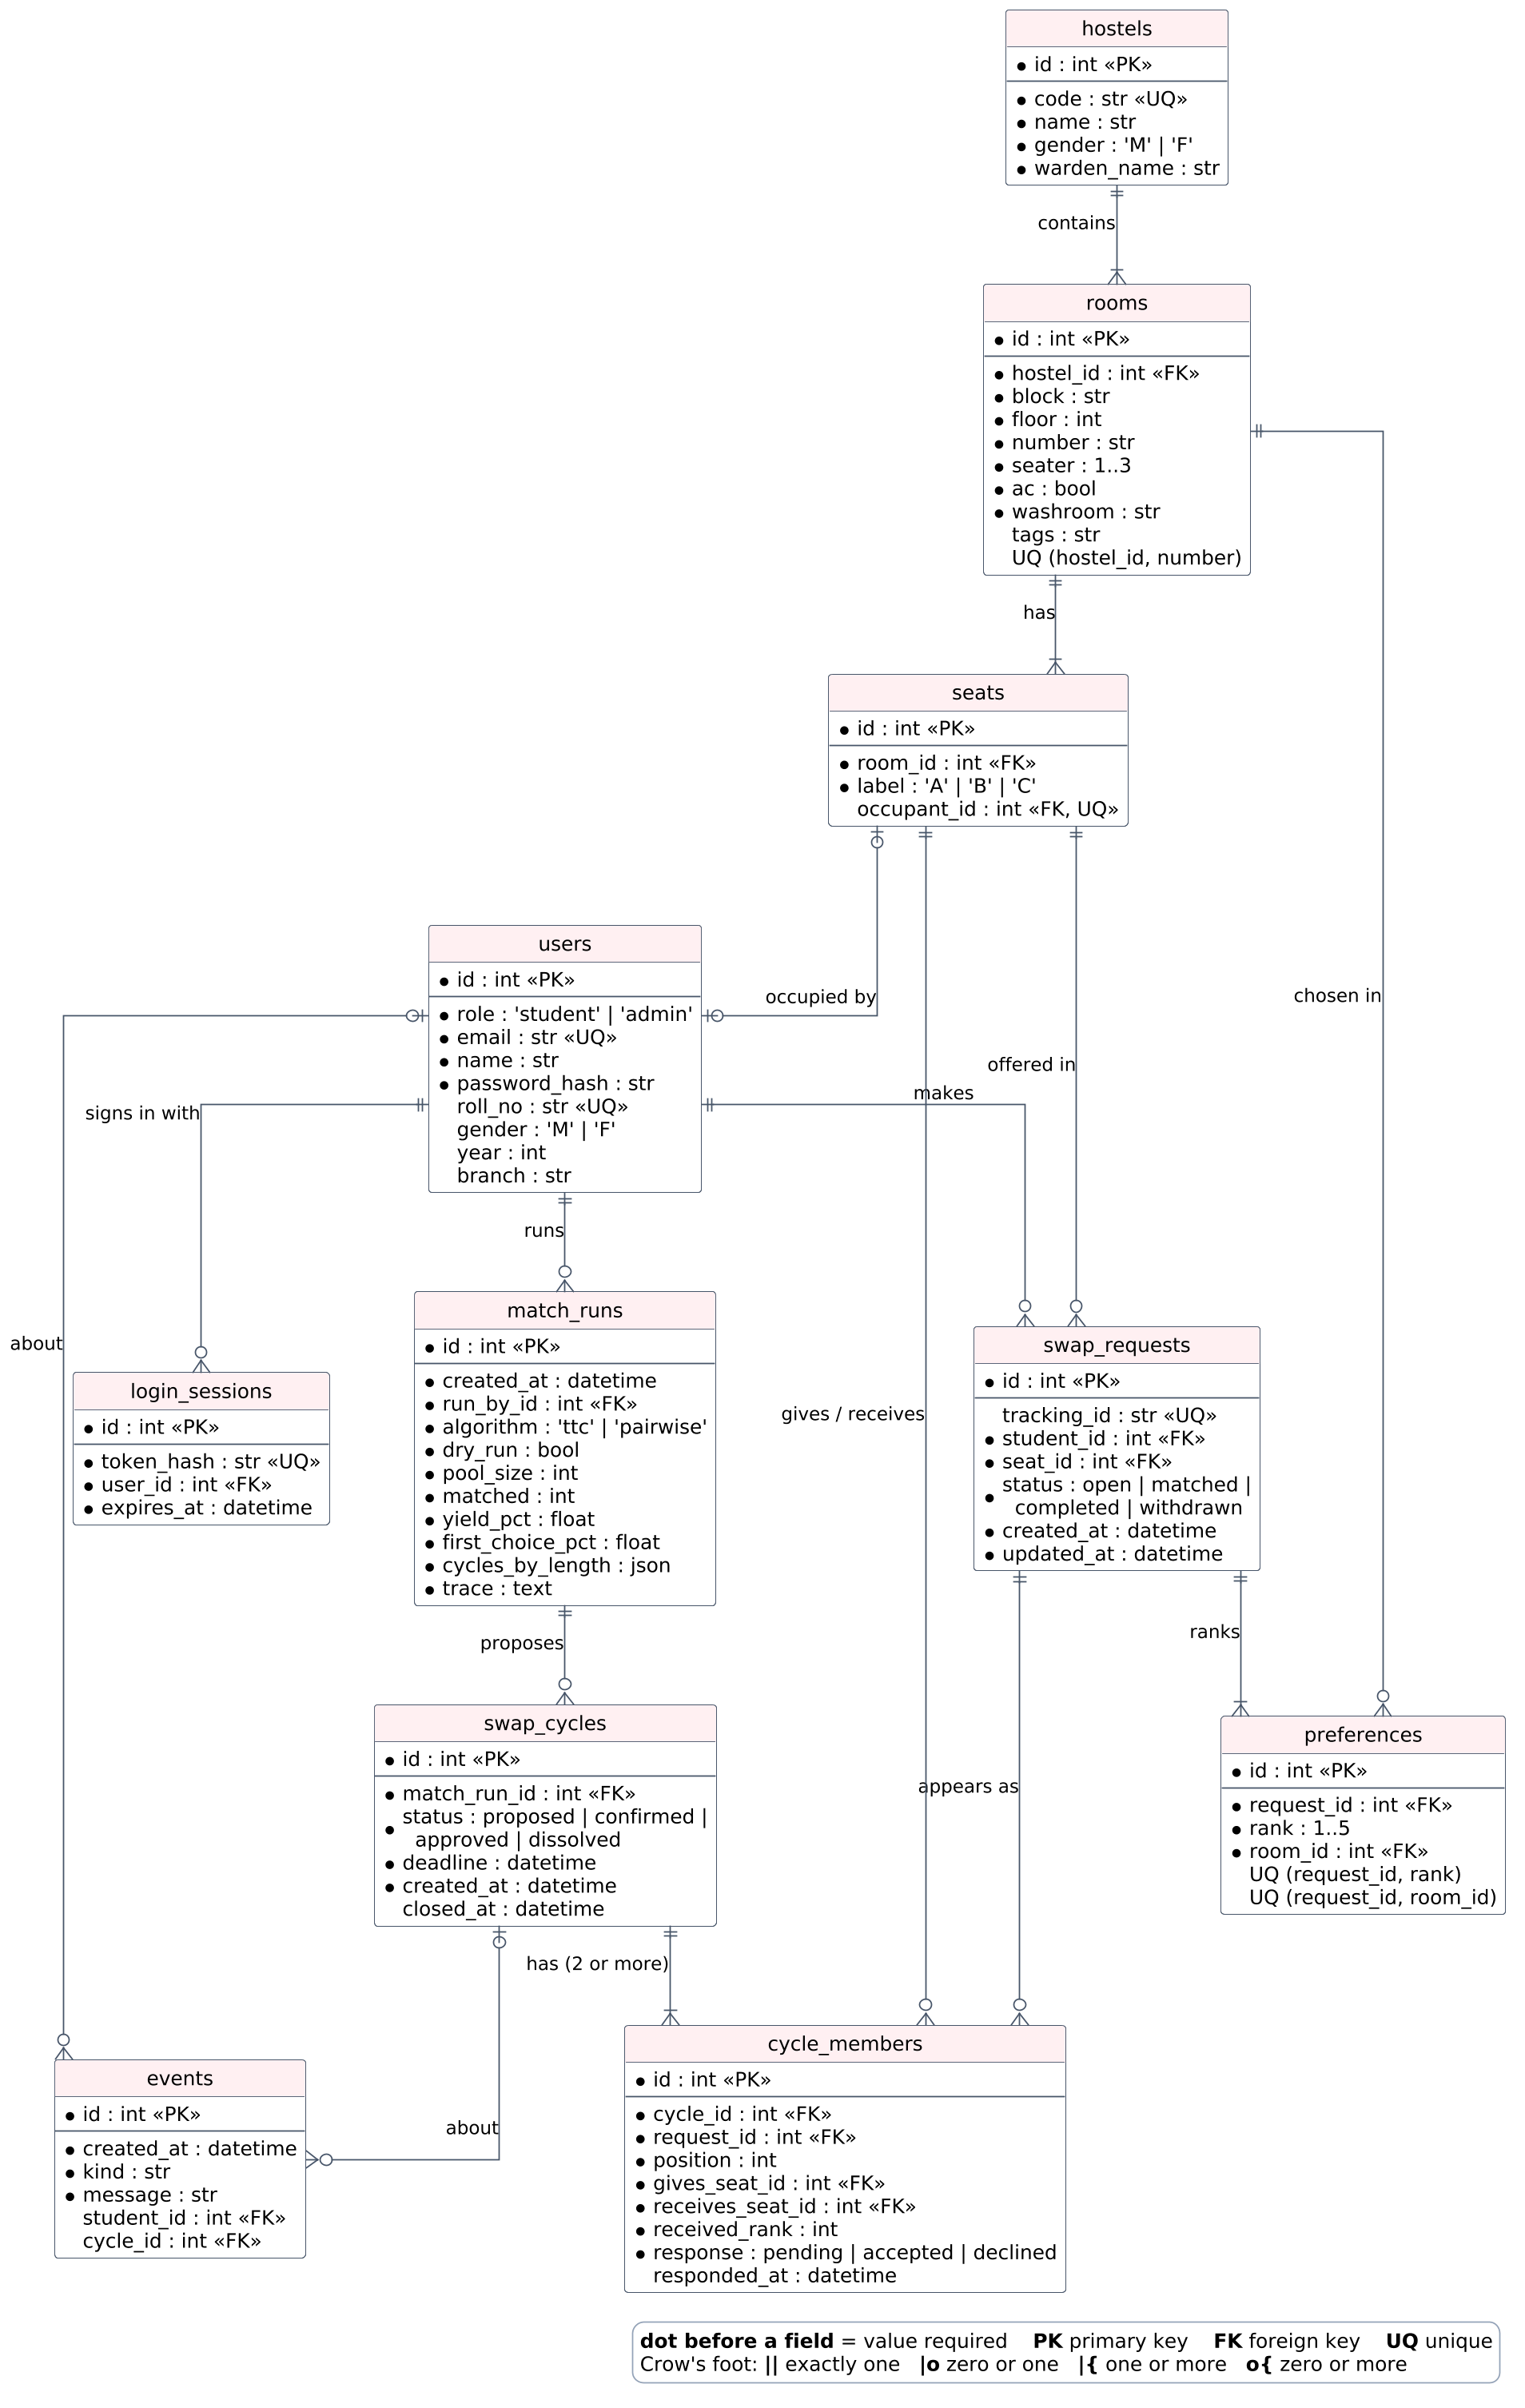
\includegraphics[width=\linewidth,height=0.88\textheight,keepaspectratio]{er}
  \caption[ER diagram]{Entity--relationship diagram of the database, in
    crow's foot notation. It mirrors \texttt{code/backend/app/models.py}.}
  \label{fig:er}
\end{figure}

\chapter{Traceability Matrix}\label{app:trace}

Each built requirement is checked by at least one automated test in
\texttt{code/backend/tests/}, or shown by a screenshot in this document.
Paths starting with \texttt{app/} or \texttt{engine/}, and \texttt{seed.py},
are under \texttt{code/backend/}; paths starting with \texttt{js/} are under
\texttt{code/frontend/public/}. Test names leave out the \texttt{test\_}
prefix. The full suite (89 tests) runs with \texttt{python -m pytest} from
the repository root.

\newcommand{\Test}[1]{{\small\ttfamily #1}}
\begin{xltabular}{\linewidth}{@{}L{2.75cm}L{4.7cm}Y@{}}
  \caption{Requirements to code and tests}\label{tab:trace}\\
  \toprule
  \textbf{Requirements} & \textbf{Code} & \textbf{Tests}\\
  \midrule
  \endfirsthead
  \toprule
  \textbf{Requirements} & \textbf{Code} & \textbf{Tests}\\
  \midrule
  \endhead
  \bottomrule
  \endlastfoot
  \Req{FR-AUTH-01, 05} & \Test{app/routers/auth.py}, \Test{app/deps.py} &
    \Test{test\_api}: \Test{login\_sets\_session\_cookie\_and\_me\_works}\\
  \Req{FR-AUTH-03} & \Test{app/routers/auth.py} & \Test{test\_api}:
    \Test{wrong\_password\_is\_rejected},
    \Test{unknown\_email\_gets\_the\_same\_answer}\\
  \Req{FR-AUTH-04} & \Test{app/routers/auth.py} & \Test{test\_api}:
    \Test{student\_using\_staff\_tab\_is\_told\_to\_switch}\\
  \Req{FR-AUTH-06} & \Test{app/routers/auth.py} & \Test{test\_api}:
    \Test{logout\_ends\_the\_session}\\
  \Req{FR-AUTH-07} & \Test{app/deps.py} & \Test{test\_api}:
    \Test{pages\_need\_login}, \Test{student\_cannot\_use\_admin\_routes}\\
  \Req{FR-AUTH-08} & \Test{js/login.js} & Figure~\ref{fig:ui-login}\\
  \midrule
  \Req{FR-ROOM-01} & \Test{app/services/views.py} &
    \Test{test\_views\_service}:
    \Test{rooms\_listing\_only\_shows\_own\_gender\_hostels}\\
  \Req{FR-ROOM-02 to 06} & \Test{app/services/views.py},
    \Test{js/rooms.js} & Figure~\ref{fig:ui-rooms}\\
  \midrule
  \Req{FR-REQ-01, 06} & \Test{app/services/requests.py} &
    \Test{test\_requests\_service}:
    \Test{submit\_saves\_ranked\_open\_request\_with\_tracking\_id}\\
  \Req{FR-REQ-02} & \Test{js/rooms.js} & Figure~\ref{fig:ui-rooms}\\
  \Req{FR-REQ-03} & \Test{app/services/requests.py} &
    \Test{test\_requests\_service}: \Test{empty\_list\_rejected},
    \Test{more\_than\_five\_rejected}, \Test{duplicate\_room\_rejected}\\
  \Req{FR-REQ-04} & \Test{app/services/requests.py} &
    \Test{test\_requests\_service}: \Test{student\_without\_seat\_rejected},
    \Test{second\_active\_request\_rejected}\\
  \Req{FR-REQ-05} & \Test{app/services/requests.py} &
    \Test{test\_requests\_service}: \Test{unknown\_room\_rejected},
    \Test{own\_room\_rejected},
    \Test{room\_in\_other\_gender\_hostel\_rejected}\\
  \Req{FR-REQ-07} & \Test{app/services/requests.py} &
    \Test{test\_requests\_service}: \Test{withdraw\_open\_request},
    \Test{withdraw\_without\_request},
    \Test{withdraw\_while\_matched\_is\_refused}; \Test{test\_api}:
    \Test{withdraw\_over\_http}\\
  \midrule
  \Req{FR-MATCH-01, 05} & \Test{app/services/matching.py},
    \Test{engine/ttc.py} & \Test{test\_matching\_service}:
    \Test{seeded\_pool\_gives\_one\_2\_3\_and\_4\_way\_chain},
    \Test{each\_member\_receives\_the\_next\_members\_seat}\\
  \Req{FR-MATCH-03} & \Test{engine/ttc.py} & \Test{test\_ttc}:
    \Test{double\_room\_seats\_are\_tried\_in\_listed\_order},
    \Test{same\_result\_whatever\_the\_input\_order}\\
  \Req{FR-MATCH-04} & \Test{engine/ttc.py} & \Test{test\_ttc}:
    \Test{random\_pools\_obey\_the\_basic\_guarantees},
    \Test{nobody\_wants\_you\_back\_means\_unmatched}\\
  \Req{FR-MATCH-06} & \Test{app/services/matching.py} &
    \Test{test\_matching\_service}:
    \Test{dry\_run\_saves\_the\_run\_but\_changes\_nothing}\\
  \Req{FR-MATCH-07} & \Test{engine/metrics.py},
    \Test{app/services/matching.py} & \Test{test\_metrics}: all three
    tests; \Test{test\_matching\_service}:
    \Test{trace\_explains\_every\_chain\_in\_plain\_words}\\
  \Req{FR-MATCH-09} & \Test{engine/pairwise.py},
    \Test{app/services/matching.py} & \Test{test\_pairwise}: all five
    tests; \Test{test\_matching\_service}:
    \Test{pairwise\_comparison\_matches\_fewer\_than\_ttc},
    \Test{pairwise\_cannot\_save\_real\_swaps}\\
  \midrule
  \Req{FR-CONF-01} & \Test{js/dashboard.js}, \Test{js/ring.js} &
    \Test{test\_views\_service}:
    \Test{dashboard\_shows\_the\_swap\_chain\_after\_matching};
    Figure~\ref{fig:ui-ring}\\
  \Req{FR-CONF-02} & \Test{app/services/cycles.py} &
    \Test{test\_cycles\_service}:
    \Test{everyone\_accepting\_confirms\_the\_cycle}\\
  \Req{FR-CONF-03} & \Test{app/services/cycles.py} &
    \Test{test\_cycles\_service}:
    \Test{one\_decline\_dissolves\_and\_returns\_others\_to\_pool}\\
  \Req{FR-CONF-04} & \Test{app/services/cycles.py} &
    \Test{test\_cycles\_service}:
    \Test{deadline\_dissolves\_unanswered\_cycles},
    \Test{answering\_after\_deadline\_is\_refused}\\
  \Req{FR-CONF-05} & \Test{app/services/cycles.py} &
    \Test{test\_cycles\_service}: \Test{outsider\_cannot\_answer},
    \Test{answering\_twice\_is\_refused}\\
  \midrule
  \Req{FR-APPR-01, 02} & \Test{app/services/cycles.py} &
    \Test{test\_cycles\_service}:
    \Test{approve\_needs\_everyone\_confirmed},
    \Test{approve\_moves\_students\_into\_their\_new\_seats}\\
  \midrule
  \Req{FR-TRACK-01, 03} & \Test{app/services/views.py} &
    \Test{test\_views\_service}: \Test{dashboard\_without\_request},
    \Test{dashboard\_with\_open\_request},
    \Test{dashboard\_after\_approval\_shows\_new\_room}\\
  \Req{FR-TRACK-04, 05} & \Test{app/services/views.py} &
    \Test{test\_views\_service}:
    \Test{admin\_overview\_reflects\_latest\_run},
    \Test{admin\_requests\_rows}\\
  \Req{FR-TRACK-06} & \Test{app/services/views.py} &
    \Test{test\_views\_service}:
    \Test{export\_csv\_has\_header\_and\_one\_row\_per\_request}\\
  \Req{FR-TRACK-07} & \Test{app/services/views.py} &
    \Test{test\_views\_service}: \Test{public\_stats\_show\_real\_counts};
    \Test{test\_api}: \Test{public\_stats\_need\_no\_login}\\
  \midrule
  \Req{NFR-PERF-01} & \Test{engine/ttc.py} & \Test{test\_ttc}:
    \Test{two\_thousand\_students\_run\_quickly}\\
  \Req{NFR-PERF-03} & all four pages & Figure~\ref{fig:ui-phone}\\
  \Req{NFR-SEC-01, 02} & \Test{app/security.py} & \Test{test\_security}:
    all five tests\\
  \Req{NFR-SAFE-05} & \Test{seed.py} & \Test{test\_seed}: all four tests\\
\end{xltabular}

\chapter{To Be Determined List}

\begin{enumerate}[label=\textbf{TBD-\arabic*},leftmargin=4.2em]
  \item The source of real hostel, room and occupancy data for a pilot,
    and who keeps it up to date.
  \item Approval to use the institute's Microsoft sign-in
    (\Req{FR-AUTH-11}).
  \item Where the system will be hosted, and who runs it.
  \item Whether 48 hours is the right confirmation deadline for the hostel
    office.
  \item How often the hostel office wants rounds to run
    (\Req{FR-MATCH-10}).
  \item The format the hostel office needs for the signed approval form
    (\Req{FR-APPR-03}).
\end{enumerate}

\end{document}
